%% BUICS THESIS STYLE for LaTeX2e
%%
%% badwanpk, Tue March 10 18:53:15 2015
%%
%% PLEASE send improvements to badwanpk at bui dot edu dot pk
%%
%%========================================
%% Commands: pdflatex tese
%%           bibtex tese
%%           makeindex tese (only if creating an index) 
%%           pdflatex tese
%%========================================

\documentclass[11pt,a4paper,oneside]{report}
\raggedbottom
\usepackage[utf8]{inputenc}
\usepackage[english]{babel}
%\usepackage[portuges]{babel}
\usepackage{fancyvrb}
\usepackage{multirow}
%\usepackage{epstopdf}
\usepackage{rotating}
\usepackage{diagbox,pict2e}
\usepackage{soul}
\usepackage{amssymb}
\usepackage{lscape}
\usepackage{longtable}
\usepackage{makeidx}
\usepackage{amsmath}
\usepackage{multirow}
\usepackage{makecell}
\usepackage{wrapfig}
\usepackage{array}
\usepackage{tabularx}
\usepackage{xcolor}
\usepackage[table]{xcolor}
\usepackage{enumitem}
\definecolor{lightgray}{rgb}{0.95, 0.95, 0.95}
\usepackage{pdflscape}
\usepackage{placeins}
\usepackage{float}
\usepackage{caption}
\usepackage{tikz}
\usetikzlibrary{positioning}
\usetikzlibrary{shapes}
\usetikzlibrary{calc}
\usepackage{fancyhdr}
\usepackage{etoolbox}
\makeatletter
\patchcmd{\@makechapterhead}
  {\vspace*{50\p@}}
  {\vspace*{0\p@}}
  {}{}
\patchcmd{\@makeschapterhead}
  {\vspace*{50\p@}}
  {\vspace*{0\p@}}
  {}{}
\makeatother

\usepackage{titlesec}
\titleformat{\chapter}[display]{\normalfont\huge\bfseries}{\chaptertitlename\ \thechapter}{20pt}{\Huge}
\titlespacing*{\chapter}{0pt}{-30pt}{20pt}
\renewcommand{\thesubsubsection}{\thechapter.\arabic{section}.\arabic{subsection}.\arabic{subsubsection}}

%% For the final version, comment next line and uncomment the second line
%\usepackage[provisional,alpharefs]{buics}
\usepackage[numericrefs]{buics} %alpharefs
\usepackage[utf8]{inputenc}

% Configure headers after all packages loaded - this overrides buics settings
\pagestyle{fancy}
\fancyhead{}
\fancyhead[R]{\leftmark}  % Chapter name in top right corner
\fancyfoot{}
\fancyfoot[C]{\thepage}  % Page number centered at bottom
\renewcommand{\headrulewidth}{0pt}
\renewcommand{\footrulewidth}{0pt}
\renewcommand{\chaptermark}[1]{\markboth{\chaptername\ \thechapter\ -- \MakeUppercase{#1}}{}}
\renewcommand{\sectionmark}[1]{}
\renewcommand{\subsectionmark}[1]{}

% Plain style for chapter first pages - NO header, only page number at bottom
\fancypagestyle{plain}{
  \fancyhead{}  % No header on first page of chapter
  \fancyfoot{}
  \fancyfoot[C]{\thepage}  % Page number centered at bottom
  \renewcommand{\headrulewidth}{0pt}
  \renewcommand{\footrulewidth}{0pt}
}

 %PDF properties 
\hypersetup{
pdftitle = {Title goes here...},
pdfauthor = {Author name},
		pdfsubject={Subject...},
    pdfcreator={MiKTex 2.9},
    pdfproducer={MiKTex 2.9},
    pdfkeywords = {Keywords},
    %pdfstartview={FitH},%fits the width of the page to the window
		pdfinfo={
    AuthorNameEnrollment1={AuthorName (Enrollment)},
		%AuthorNameEnrollment2={AuthorName (Enrollment)},%%uncomment this line if 2 authors
		Supervisor={SupervisorName (Designation)},
    Session={Fall 2015},%%Session in which the defense was arranged (Spring / Fall 20XX)
		InternalExaminer={Dr. ABC (Designation)},
		ExternalExaminer={Dr. XYZ (Designation)},
		ProjectCoordinator={Dr. XYZ (Designation)},
		HOD={Dr. XYZ (Designation)},
		DefenseDate={\today},
  }
}

%% Options: 
%% - english: titles, etc in english
%% - provisional: the thesis has not been approved yet
%% - print: links are not shown (for paper versions)
%% - alpharefs: bibliography references are alphabetic
%% - numericrefs: bibliography references are numbered (in order of citation)
%% ( by default: author-date format of the ``natbib'' package is used 


%% Provide a version number in order to keep track of
%% thesis versions (it will printed in the footer of most pages)

\version{v1.12.2015}

%% uncomment in the final version in order to make version footer disappear
%\noversiontrue

%% uncomment to create an index (at the end of the document)
\makeindex 

%%  path to the figures directory
%%  TIP: use folder ``figures'' to keep all your figures
\graphicspath{{figures/}}

%%----------------------------------------
%% TIP: if you want to define more macros, use an external file to
%% keep them
%some macro definitions

% format
\newcommand{\class}[1]{{\normalfont\slshape #1\/}}

% entities
\newcommand{\Feup}{Faculdade de Engenharia da Universidade do Porto}

\newcommand{\svg}{\class{SVG}}
\newcommand{\scada}{\class{SCADA}}
\newcommand{\scadadms}{\class{SCADA/DMS}}

%%----------------------------------------

%%========================================
%% Start of document
%%========================================
\begin{document}

%%----------------------------------------
%% Information about the work
%%----------------------------------------
\title{Indus Bazar – A B2B Marketplace Application}
\author{
    \begin{tabular}{c}
        {\sc Husnain Nadeem} \\
       01-135222-060 \\
        \\
        {\sc Kashan Mehmood} \\
        01-135222-008 \\
    \end{tabular}
}

\degree{\textbf{\Large{Bachelor of Science in Information Technology}}}
%\degree{\emph{Thesis submitted to the Department of Computer Science, Bahria University, Islamabad\\for fulfillment of the requirements of Bachelors of Science in Computer Science degree.}}
%% Date of submission
\vspace{-0.5cm} 
\department{Department of Computer Science\\Bahria University, Islamabad}
\thesisdate{April 2026}
%\thesisdate{\Large{\textbf{September 2012}}}



%% uncomment next line if necessary
\supervisor{Supervisor}{Sir Raja Shamayel Ullah}{}% {(Title)}

% uncomment committee stuff in the final version if used

\certificatetext{We accept the work contained in the report title “Indus Bazar – A B2B Marketplace Application” written by Mr.Husnain Nadeem  and Mr.Kashan Mehmood as a confirmation to the required standard for the partial fulfillment of the degree of Bachelor of Science in Computer Science.}

\committeetext{Approved by \ldots:}

\committeemember{Supervisor}{Sir Raja Shamayel Ullah}{(Sr.Lecturer)}
\signature
\committeemember{Internal Examiner}{Name of the Internal Examiner}{(Title)}
\signature
\committeemember{External Examiner}{Name of the External Examiner}{(Title)}
\signature
\committeemember{Project Coordinator}{Dr. Kabeer Ahmed Bhatti}{(Fyp Coordinator IT Department)}
\signature
\committeemember{Head of the Department}{Dr. Muhammad Khurram Ehsan}{(Head Of Department Computer Science)}
\signature
\committeedate{April , 2026}

%% specify cover logo (in folder ``figures'')
\logo{BUI-Logo}

%%----------------------------------------
%% Cover page(s)
%%----------------------------------------
\maketitle
%% uncomment next line in the final version if used
\committeepage

%% Preliminary materials
\StartPrelim
\pagestyle{plain}  % No headers for preliminary pages
\begin{singlespace}
  \chapter*{Abstract}
\addcontentsline{toc}{chapter}{Abstract}

Bulk trading inefficiencies, lack of digital connectivity, and reliance on manual, trust-based processes are some of the major challenges increasingly faced by businesses in Pakistan, particularly among small and medium enterprises. These issues often remain unaddressed due to the absence of localized digital platforms tailored to the needs of the Pakistani market. The Indus Bazar system provides a mobile-based, interactive B2B marketplace that simplifies bulk trading by connecting manufacturers, wholesalers, and retailers within a unified digital environment where they can communicate, negotiate, and complete transactions securely in both Urdu and English. The platform incorporates advanced features such as real-time chat, tiered pricing, intelligent product search, and AI-generated review insights to support transparent and efficient business operations.The system is specifically designed to overcome the limitations of traditional e-commerce platforms that mainly focus on end consumers and fail to address the cultural and operational needs of business-to-business interactions in Pakistan. By offering an intuitive and culturally aligned interface, Indus Bazar enables enterprises to establish trusted connections, manage bulk orders, and expand their business operations digitally without relying on unnecessary intermediaries.Moreover, the platform integrates modern technologies such as Flutter and Appwrite, along with secure payment processing through Stripe, to deliver a fast, reliable, and scalable user experience. Its real-time communication system, notification features, and secure authentication ensure seamless interaction while maintaining data privacy and transaction safety. Future enhancements include incorporating AI-driven demand forecasting to further optimize trade efficiency.This project is developed as an industrial initiative by Rainy Sports, aiming to leverage its industry experience to bridge the gap between traditional trading practices and modern digital solutions. Through this initiative, Rainy Sports seeks to contribute to the digital transformation of Pakistan’s business ecosystem by providing a practical, scalable, and user-centric platform for bulk trade.The project ultimately aims to empower Pakistani businesses by promoting trust, strengthening local supply chains, and supporting the growth of a digitally connected economy.
 % the abstract
  \chapter*{Acknowledgments}
%\addcontentsline{toc}{chapter}{Acknowledgments}

We would like to express our sincere gratitude to our respected project supervisor, Mr. Raja Shumayel, Faculty Member at Bahria University, for his continuous guidance, valuable insights, and unwavering support throughout the development of this project. His constructive feedback and encouragement played a vital role in shaping both the direction and successful completion of our Final Year Project. We are especially thankful for his involvement during the early stages, where we identified a significant market gap and refined our idea into a practical and impactful solution under his supervision.We would also like to extend our appreciation to our Company Supervisor, Mr. Muhammad Rizwan Mirza, Partner at Rainy Sports, for his professional guidance and industry-oriented perspective. As this project is carried out as an industrial initiative, his insights into real-world business processes, market challenges, and operational requirements greatly contributed to the practicality and relevance of our system. His support helped bridge the gap between academic concepts and industry implementation.
We also take this opportunity to thank all those who indirectly contributed to our research by providing insights into the challenges faced in the local business ecosystem, which helped us better understand real-world problems and design a system aligned with market needs. We are particularly grateful to all the participants and contributors who supported our research process by sharing their perspectives and experiences. Their input was essential in validating the practicality and relevance of our proposed system.
We would also like to acknowledge the Department of Computer Science, Bahria University, for providing us with the necessary academic resources, technical facilities, and a supportive environment that enabled us to carry out this project effectively.
Lastly, we extend our heartfelt thanks to our families and friends for their constant encouragement, patience, and moral support throughout this challenging yet rewarding journey. Their belief in us kept us motivated and focused until the successful completion of this project.

\vspace{10mm}

\flushleft{\textsc{Husnain Nadeem, Kashan Mehmood} \\Islamabad, Pakistan}

\flushleft{April 2026}
  % the acknowledgments
  \cleardoublepage
\thispagestyle{plain}

\vspace*{8cm}

\begin{flushright}
   \textsl{``We think someone else, someone smarter than us,\\someone more capable, someone with more resources will solve that problem.\\But there isn't anyone else.''} \\
\vspace*{1.5cm}
            Regina Dugan
\end{flushright}
    % initial quotation if desired
  \clearpage
  \pdfbookmark[0]{Table of Contents}{contents}
  \tableofcontents
  \clearpage
  \pdfbookmark[0]{List of Figures}{figures}
  \listoffigures
  \clearpage
  \pdfbookmark[0]{List of Tables}{tables}
  \listoftables
  \chapter*{Acronyms and Abbreviations}
%\addcontentsline{toc}{chapter}{Abbreviations}
\chaptermark{Acronyms and Abbreviations}

\begin{flushleft}
\begin{tabular}{l p{0.8\linewidth}}
AI & Artificial Intelligence\\
API & Application Programming Interface\\
B2B & Business-to-Business\\
BaaS & Backend-as-a-Service\\
ERD & Entity Relationship Diagram\\
FCM & Firebase Cloud Messaging\\
GUI & Graphical User Interface\\
HLD & High Level Design\\
HTTPS & Hypertext Transfer Protocol Secure\\
iOS & iPhone Operating System\\
JSON & JavaScript Object Notation\\
LLD & Low Level Design\\
NoSQL & Not Only SQL\\
PCI & Payment Card Industry\\
PKR & Pakistani Rupee\\
REST & Representational State Transfer\\
RFQ & Request for Quotation\\
RLS & Row-Level Security\\
SDK & Software Development Kit\\
SME & Small and Medium Enterprise\\
UC & Use Case\\
UI & User Interface\\
UML & Unified Modeling Language\\

\end{tabular}
\end{flushleft}  % the list of abbreviations used
\end{singlespace}

%%----------------------------------------
%% Body
%%----------------------------------------
\StartBody

% Re-configure fancy headers for chapters
\pagestyle{fancy}
\fancyhead{}
\fancyhead[R]{\leftmark}  % Chapter name in top right corner
\fancyfoot{}
\fancyfoot[C]{\thepage}  % Page number centered at bottom
\renewcommand{\headrulewidth}{0pt}
\renewcommand{\footrulewidth}{0pt}

%% TIP: use a separate  file for each
\chapter{Introduction} \label{chap:intro}
The manufactured goods supply chain in Pakistan is highly fragmented, forcing businesses to deal with various intermediaries, which makes it run at higher costs, delays, and non-transparently \cite{hussain2023supply,raza2023impact}. The current e-commerce platforms primarily target end consumers and do not consider the unique requirements of business-to-business dealings in the local market \cite{ali2022ecommerce,laudon2023ecommerce}. It forms a loophole to a localized digital solution that will enable simplifying bulk trading and enhancing supply chain efficiency. In order to overcome this problem, Indus Bazar is created as a mobile B2B marketplace that links manufacturers, wholesalers, and retailers in a single digital marketplace \cite{han2023digital,farooq2024mobile}. It allows users to interact, bargain and transact easily in Urdu and English, in line with best practices in designing multilingual and culturally sensitive user experience designs \cite{akram2022user,shaikh2024design}. The platform has such essential features as real-time chat, tiered pricing, smart product searches, and AI-powered review insights to help facilitate transparent and efficient trade and make them less reliant on intermediaries. Modern technologies such as Flutter (Cross-platform), Dart (Application Logic), and Appwrite (Backend Services) are used to construct Indus Bazar, as well as secure payment creation through Stripe, which is also consistent with modern digital commerce architecture designs \cite{chaffey2022digital}. Additional functionalities such as real-time notification, secure log-in, Request for Quotation (RFQ) enable both the buyer and sellers to interact more. On the whole, the platform will empower Pakistani businesses by fostering trust, enhancing access to supply chains and, potentially, in the future, AI-driven analytics and demand forecasting that will drive economic growth through digitization of the Pakistani economy.
\section{Project Background}
The classical Pakistani business environment, especially in the wholesale and bulk trade area, is heavily reliant on the manual processes, personal connections, and trust relations \cite/supply|). Small and medium enterprises usually have serious issues when it comes to getting products directly with manufactures as they have to go through various intermediaries. This does not only add more expenses to the procurement process but also causes delays alongside reducing transparency within the supply chain \cite{raza2023impact}. Although digital technologies are getting developed quickly, the majority of existing e-commerce platforms are implemented with consumer markets in mind and fail to meet the needs of business-to-business transactions in particular \cite{ali2022ecommerce,laudon2023ecommerce}.
As the digital transformation in commerce gains demands, the need to have platforms that can streamline business interactions and direct access between suppliers and buyers is on the rise \cite{han2023digital}. This is further emphasized by the lack of a localized, user-friendly, and culturally focused B2B market in Pakistan, especially within the context of language and usability \cite{akram2022user,nielsen2020usability}. Businesses need a system that helps to not only facilitate transactions, but also facilitates communication, negotiation and long-term relationship construction in a safe and efficient way \cite{zafar2022trust}.
Indus Bazar was planned based on comprehensive research and the realization of an apparent gap in the market in terms of accessibility and effectiveness of bulk trading systems in Pakistan \cite{worldbank2023pakistan}. This concept was also developed further by engaging in in-depth consultation with our project supervisor whose advice aided in developing the concept into a feasible and effective solution. With the application of modern technologies and incorporation of key business elements, the platform will help streamline the supply chain processes, decrease the reliance on the intermediaries, and allow businesses to work more effectively in a digitally integrated world. The project is a developed industrial project in partnership with Rainy Sports. It has real-life business needs and will provide practical solution based on the needs of the industry.


\section{Problem Description}
The conventional B2B e-commerce in Pakistan has serious constraints related to small and medium enterprises that are involved in bulk trade \cite{han2023digital}. The majority of platforms are mainly targeting end consumers and do not offer a real-time communication between buyers and sellers, which is crucial in the establishment of trust in local business transactions -ali2022ecommerce,zafar2022trust. This becomes problematic because of the absence of features like tiered pricing on bulk orders as well as real-time notifications and chat features, which commonly result in delayed responses, lost business opportunities, and procurement inefficiencies \cite{chaffey2022digital}. Also, the available solutions are either too complicated to use by small sellers or too simple to use by expanding businesses, leaving a market gap in the middle ground between the two extremes that can efficiently work together. A lot of platforms do not support culturally relevant practices and multilingual support either, as businesses can still use traditional methods and intermediaries that add to the expenses and decrease the level of transparency \cite{akram2022user,shaikh2024design}. It complicates the process of accessing suppliers directly by small retailers and wholesalers and prevents their ability to compete with larger businesses. There exists an obvious necessity of the B2B solution that should be scaled, intuitive and locally oriented to enable the efficient interaction, secure transactions, and transparent trade. A platform like this would enable companies to handle orders, negotiate, and sustain relationships with suppliers and buyers in a streamlined digital space \cite{laudon2023ecommerce}. By focusing on these issues, the platform will be able to minimize the use of intermediaries, reduce operational expenses, enhance supply chain effectiveness, and enable Pakistani businesses to expand in a more digitally connected economy \cite{worldbank2023pakistan}. To address this gap, Indus Bazar is created as a complete B2B marketplace, which will offer real-time communication, flexible pricing, intelligent search of products, and AI-based insights to make transactions more transparent, trustful, and efficient.
\section{Project Objectives}
The project intends to design and develop a holistic, secure and multi-purpose e-commerce site specific to the Pakistani market. The platform aims to enable smooth B2B dealings between customers, sellers, and manufacturers and offer contemporary, user-friendly and culturally befitting online trading experiences. With the incorporation of modern technologies, the system will promote efficiency, interaction and confidence in Web-based dealings, minimize intermediaries in supply chains and enable both large and small businesses to conduct business in a virtual market space.

\section*{The Most Important Goals of the Project will be to:}
\begin{itemize}
\item Traditional multi-role platform used by the manufacturers, wholesalers, retailers and individual customers, which have role-based access control such that all users are granted specific and appropriate permissions.
\item Support easy B2B transactions: provide real-time communication, negotiations and cooperation between buyers and sellers.
\item Develop a current payment system that supports a tiered pricing strategy, secure payments and other payment systems suitable to the local market. As of now, the system is linked to Stripe in its test mode to re-create the secure payments transactions and test the payment process.
\item Add AI-driven functionality will give terse sentences based on customer reviews, which will assist sellers to have a better visualization of feedback and improve their products and services within a short time. Currently, AI aspect is limited to review summarization.
\item Build a mobile Android application in Flutter that is device friendly and easy to use.
\item Develop a sophisticated product management system that has intelligent search and filtering features that enable users to easily locate and manage products.
\item Add real-time chat policy to offer direct offers and bargains in between purchasers and sellers.
\item Improve an effective order management system to make it easier to buy and deliver.
\item Ensure that the platform is secure by offering effective authentication, authorization and data protection measures to secure user accounts and other sensitive data.
\item Provide a culturally aware online shopping experience that addresses the unique requirements of the Pakistani market, as well as reduces the importance of the middlemen in the supply chain.
\end{itemize}
\section{Project Scope}

The design and development of an entire B2B e-commerce platform to establish a seamless interaction between the buyers and manufacturers will be covered as part of the work plan of \textbf{Indus Bazar -A B2B Marketplace Application. The system provides a secure multi-role access, stream purchase operations, smart product management and real-time communication to enhance the overall user experience.The project is dedicated to development of a mobile based marketplace which has a multi role authentication, safe email verification, and password recovery. It will possess an already developed product line with advanced search and filtering, shopping cart and checkout with secure Stripe (Test Mode) payments. Positional order management system assists the whole order process including purchases with in-bulk prices through levels of tiered pricing.The website also provides the ability to handle addresses to deliver, provide feedback and view AI-generated feedbacks summaries in English and Urdu. It also has real-time chat (buyer-seller communication), and push notification (timely update about orders and activities in the system). Pakistani users can access it thanks to multilingual support, and have an easy experience.

\subsection{Goals}
\begin{itemize}
    \item Develop a secure and scalable mobile application of e-commerce between manufacturers and buyers (B2B).
    \item Facilitate easy product discovery with sophisticated search and filtering functionalities.
    \item Facilitate mass purchases through tiered pricing system.
    \item Provide an easy and trouble-free shopping cart and check-out.
    \item Implement secure online payment processing with Stripe.
    \item Facilitate live interaction between buyers and sellers.
    \item Summarize product reviews in English and Urdu with the help of AI.
    \item Enforce user privacy, authentication and access control.
    \item Support multilingual interaction to make it simpler to Pakistani users.
    \item Enable sellers to effectively deal with products, orders, and customer relations.
    \item Provide real-time order, chat, and system-notifications.
\end{itemize}

\subsection{Features}
\begin{enumerate}

    \item \textbf{Authentication and Role-Based Onboarding entity.} \\
    Email-verifies registration and authenticates customers and sellers via deep linking and password recovery

    \item \textbf{Product Catalog Management} \\
    Provides a search system, filtering and tier pricing to allow the user to conveniently search and purchase products.

    \item \textbf{Shopping Cart and Checkout} \\
    Allows consumers to add items to cart, specify delivery address and process the order by use of streamlined checkout process.

    \item \textbf{Secure Payment Integration} \\
    Integrates Stripe payment gateway through server-side operations in order to have secure and reliable transactions.

    \item \textbf{Order Management System} \\
    Deals with all lifecycle of orders including ordering, tracking, updates and status of orders.
    
    \item \textbf{Seller Dashboard} \\
    Provides sellers with the ability to manage products, monitor orders and perform Order-related actions.

    \item \textbf{Real-Time Chat System} \\
    Enables real time communication between individuals selling and buying goods and services, including text and image communications.

    \item \textbf{RFQ (Request for Quotation) Marketplace} \\
    Gives customers a chance to make requisitions on items, accept an offer of vendors and conduct transactions as per the preferred offers.
    
    \item \textbf{AI-Powered Review Summarization} \\
    Creates short-overviews of AI-customer-reviews in English and Urdu to come up with more applicable decisions.

    \item \textbf{Push Notifications} \\
    Incorporates Firebase and Appwrite messaging services to provide real-time updates messages concerning the changes in the orders, chat messages, and system messages.

    \item \textbf{Delivery Address Management} \\
    Enables the user to create, update and maintain numerous delivery addresses.

    \item \textbf{Multilingual Support} \\
    Delivers a good sense of familiarity and localization by using either English language or Urdu.

\end{enumerate}

\subsection{User-Friendly Mobile Application Design.}
\begin{itemize}
    \item \textbf{Built with Flutter (Dart)} \\
    Enables cross-platform, high-performance mobile application and a consistent user experience.

    \item \textbf{Easy and User-Friendly Interface} \\
    Offers a simplified navigation with well-defined structures and simplified work processes.

    \item \textbf{Interactive and Responsive Design} \\
    Improves the experience of users with real-time chat and notification and dynamic UI components.

    \item \textbf{Scalable Architecture} \\
     Employs Appwrite back-end, Riverbed state management, and modular service layers to be maintainable and scalable.

\end{itemize}

%%more details about figures can be found on https://en.wikibooks.org/wiki/LaTeX/Floats,_Figures_and_Captions
 
\chapter{Literature Review and Existing Systems} \label{chap:literatureReview}
%\version{v1.10.2015}

Digital transformation of Business-to-business (B2B) commerce in Pakistan has been identified as a key facilitator to SMEs growth and supply chain optimization \cite{han2023digital}. Studies show that the adoption of e-commerce by Pakistani businesses, though on the rise, is still below global standards, and the current platforms mostly do not meet the needs of the local level of localization \cite{ali2022ecommerce}. The digitization of the supply chain in developing countries such as Pakistan is a major opportunity to cut the number of intermediaries and operational expenses \cite{hussain2023supply}. Mobile applications have played a significant role in boosting B2B trading within developing markets, which is accessible and convenient to use \cite{farooq2024mobile}. Nonetheless, Pakistani SMEs, which are online transaction users, still prioritize trust and security as the primary concerns of online transactions \cite{zafar2022trust}. Accelerated digital transformation is considered to be the driving force behind economic growth in the report of the World Bank on the digital economy \cite{worldbank2023pakistan}. Locally oriented B2B platforms in South Asian markets are promising in terms of regional barriers overcome \cite{shaikh2024design}. Although traditional, intermediaries still influence the efficiency of wholesale trade, and direct digital connections are necessary to eliminate their influence on efficiency and efficiency in wholesale trade transactions \cite{raza2023impact}. The adoption of the platform in Pakistan depends on the multilingual interface and user experience design that is culturally appropriate \cite{akram2022user}. Modern online trading platforms need to strike a balance between usability-engineering, and business model strategy on the internet, combining both new technology and simplicity and accessibility by a variety of business users.

\section{B2B E-Commerce in South Asia.}

The B2B e-commerce market in South Asia, especially in Pakistan, is a major growth potential having a huge untapped potential. The old system of wholesale and bulk trading has been based on personal relations and personal contact, which has introduced inefficiencies and reduced the accessibility of markets to the traditional system of these relations and contacts \cite{ali2022ecommerce}. This landscape is radically changing with digital market places that facilitate transparent pricing, expanded market reach, and effective order management. The use of these platforms is influenced by various factors such as increased internet penetration, the availability of smartphones, and increasing digital literacy of business professionals \cite{farooq2024mobile}. Modern studies show that B2B mobile-first solutions purpose-built to cater to emerging markets are capable of reaching a greater adoption rate than generic ones can reach \cite{shaikh2024design}. Regional B2B platforms require critical knowledge of the local business practices, payment preferences, and communication protocols to be successful \cite{hussain2023supply}.

\section{Important Research Areas of B2B Digital Transformation.}

\subsection{Digital Transformation and SME Challenges}
Small and medium enterprises in Pakistan face multifaceted challenges in embracing digital transformation. According to a study conducted by Han and Ahmed (2023) \cite{han2023digital}, the main obstacles include a shortage of capital investment, absence of technical skills, and opposition to change in the conventional business cultures. Nevertheless, the companies, which manage to implement digital solutions successfully, witness the objective improvement of the efficiency of their work and gain access to new markets. This paper highlights the need to come up with platforms that take into account these limitations and offer concrete value propositions to encourage adoption.

\subsection{Trust, Security, and User Confidence}
Successful adoption of B2B market places is anchored on user trust. According to Zafar and Malik (2022) \cite{zafar2022trust}, an empirical investigation of Pakistani SMEs revealed that secure authentication systems, transparent ratings of sellers, and effective payment systems play a crucial role in user confidence in online transactions. Their study underscores the fact that the implementation of security should be moderate and convenient enough to make the platform accessible to many. Moreover, safe data protection and adherence to the local regulations increases the market credibility.

\subsection{Mobile-First Architecture for Market Access}
The importance of mobile applications in the emerging market commerce is critical and is well-documented. Farooq and Khan (2024) \cite{farooq2024mobile} reveal that mobile-first constructions in developing markets record 40 percent greater engagements in comparison with desktop-centered remedies. Their analysis highlights how mobile apps can be used to access business in remote locations with inadequate infrastructure, democratizing the market to smaller businesses.

\subsection{Multilingual and Localized User Experience}
The design of user experience in multilingual environments must be very sensitive to language, cultural and contextual issues. Akram and Latif (2022) \cite{akram2022user} provide the best practices in the designing of mobile applications that support multiple languages such as Urdu and English. According to their study, the culturally appropriate design enhances user adoption by 35 percent and learning curves are much lower.

\section{Comprehensive Literature Review}

The table below (ref. tab:literature review) is a synthesized summary of prominent academic literature and publications associated with B2B e-commerce, digital transformation and marketplace design, which are the theoretical basis of the Indus Bazar development.

\renewcommand{\arraystretch}{1.3}
\small
\begin{longtable}{|>{\raggedright}p{1.8cm}|>{\raggedright}p{3cm}|>{\centering}p{0.8cm}|>{\raggedright}p{2cm}|>{\raggedright\arraybackslash}p{4.5cm}|}
\caption{B2B E-Commerce Research and Related Studies}
\label{tab:literature_review}\\
\hline
\rowcolor{lightgray}
\textbf{Author(s)} & \textbf{Title} & \textbf{Year} & \textbf{Source} & \textbf{Key Findings} \\
\hline
\endfirsthead

\hline
\rowcolor{lightgray}
\textbf{Author(s)} & \textbf{Title} & \textbf{Year} & \textbf{Source} & \textbf{Key Findings} \\
\hline
\endhead

\hline
\endfoot

\hline
\endlastfoot

Hussain, M. \& Iqbal, Z. & Supply Chain Digitization in Developing Economies: Evidence from Pakistan\cite{hussain2023supply} & 2023 & International Journal of Supply Chain Management & Digitized supply chains reduce costs by 25-30\% and improve transparency; intermediary elimination through direct digital connections is economically viable. \\
\hline

Raza, S. \& Siddiqui, A. & Impact of Intermediaries on Wholesale Trade Efficiency in Pakistan\cite{raza2023impact} & 2023 & Asian Journal of Business Research & Intermediaries increase product costs by 15-20\%; direct digital connections between suppliers and retailers significantly improve margin optimization. \\
\hline

Ali, S. \& Rehman, M. & E-commerce Adoption in Pakistan: A Study of Business-to-Business Platforms\cite{ali2022ecommerce} & 2022 & Pakistan Journal of Commerce and Social Sciences & Existing B2B platforms lack localization and culturally aligned features; there is significant market demand for platforms addressing local business practices and payment methods. \\
\hline

Laudon, K. C. \& Traver, C. G. & E-commerce: Business, Technology, Society\cite{laudon2023ecommerce} & 2023 & Pearson (Book - 17th ed.) & Comprehensive framework for analyzing digital commerce ecosystems, including technological, social, and regulatory dimensions critical for platform success. \\
\hline

Han, R. \& Ahmed, T. & Digital Transformation of SMEs in Pakistan: Challenges and Opportunities\cite{han2023digital} & 2023 & Journal of Entrepreneurship and Business Innovation & SMEs in Pakistan face capital and expertise constraints; digital solutions must be cost-effective and easy to implement for successful adoption. \\
\hline

Farooq, U. \& Khan, A. & Role of Mobile Applications in Enhancing B2B Trade in Emerging Markets\cite{farooq2024mobile} & 2024 & International Journal of Information Systems & Mobile platforms show 40\% higher engagement in emerging markets; accessibility in remote areas is critical for inclusive growth. \\
\hline

Akram, W. \& Latif, H. & User Experience Design for Multilingual Mobile Applications in Pakistan\cite{akram2022user} & 2022 & International Journal of Human-Computer Interaction & Multilingual interfaces increase adoption by 35\%; culturally appropriate design reduces learning curves and enhances user retention. \\
\hline

Shaikh, N. \& Qureshi, F. & Design and Implementation of Localized B2B Platforms for South Asian Markets\cite{shaikh2024design} & 2024 & Journal of Software Systems and Applications & Localized platforms addressing regional preferences achieve higher adoption; considerations for payment methods, languages, and business protocols are essential. \\
\hline

Chaffey, D. & Digital Business and E-commerce Management\cite{chaffey2022digital} & 2022 & Pearson (Book - 8th ed.) & Holistic approach to digital commerce strategy covering customer experience, digital channels, data analytics, and organizational change management. \\
\hline

World Bank & Pakistan Digital Economy Report: Accelerating Digital Transformation\cite{worldbank2023pakistan} & 2023 & World Bank Publications & Pakistan's digital economy growing at 18\% annually; digital transformation is essential for economic competitiveness and SME growth. \\
\hline

Nielsen, J. & Usability Engineering for E-commerce Platforms\cite{nielsen2020usability} & 2020 & Morgan Kaufmann (Book) & Simplified navigation, clear information architecture, and intuitive checkout processes reduce cart abandonment and increase conversion rates. \\
\hline

Zafar, H. \& Malik, S. & Trust and Security in Online Marketplaces: A Study of Pakistani SMEs\cite{zafar2022trust} & 2022 & Journal of Cybersecurity and Digital Trust & Security, seller ratings, and transparent payment systems are critical for user trust; localized security practices enhance platform credibility. \\
\hline

Porter, M. E. & Strategy and the Internet\cite{porter2001strategy} & 2001 & Harvard Business Review & Digital platforms fundamentally reshape competitive dynamics; success requires alignment of technology with sustainable business strategy. \\

\end{longtable}
\normalsize

\section{Analysis of Existing B2B Systems}

In the pursuit of a gap analysis and competitive analysis, we examine three existing B2B marketplace solutions that are already in operation in Pakistan and South Asia.

\subsection{System 1: TradeHub Pakistan}

TradeHub Pakistan is a B2B web-based marketplace, which has been in operation since 2019 and is aimed at matching manufacturers with bulk buyers. The site provides product descriptions, simple search services and emailing options between the consumers and the merchants. It favors credit-based system of payments and offers catalog management portal to sellers.

\begin{figure}[H]
    \centering
    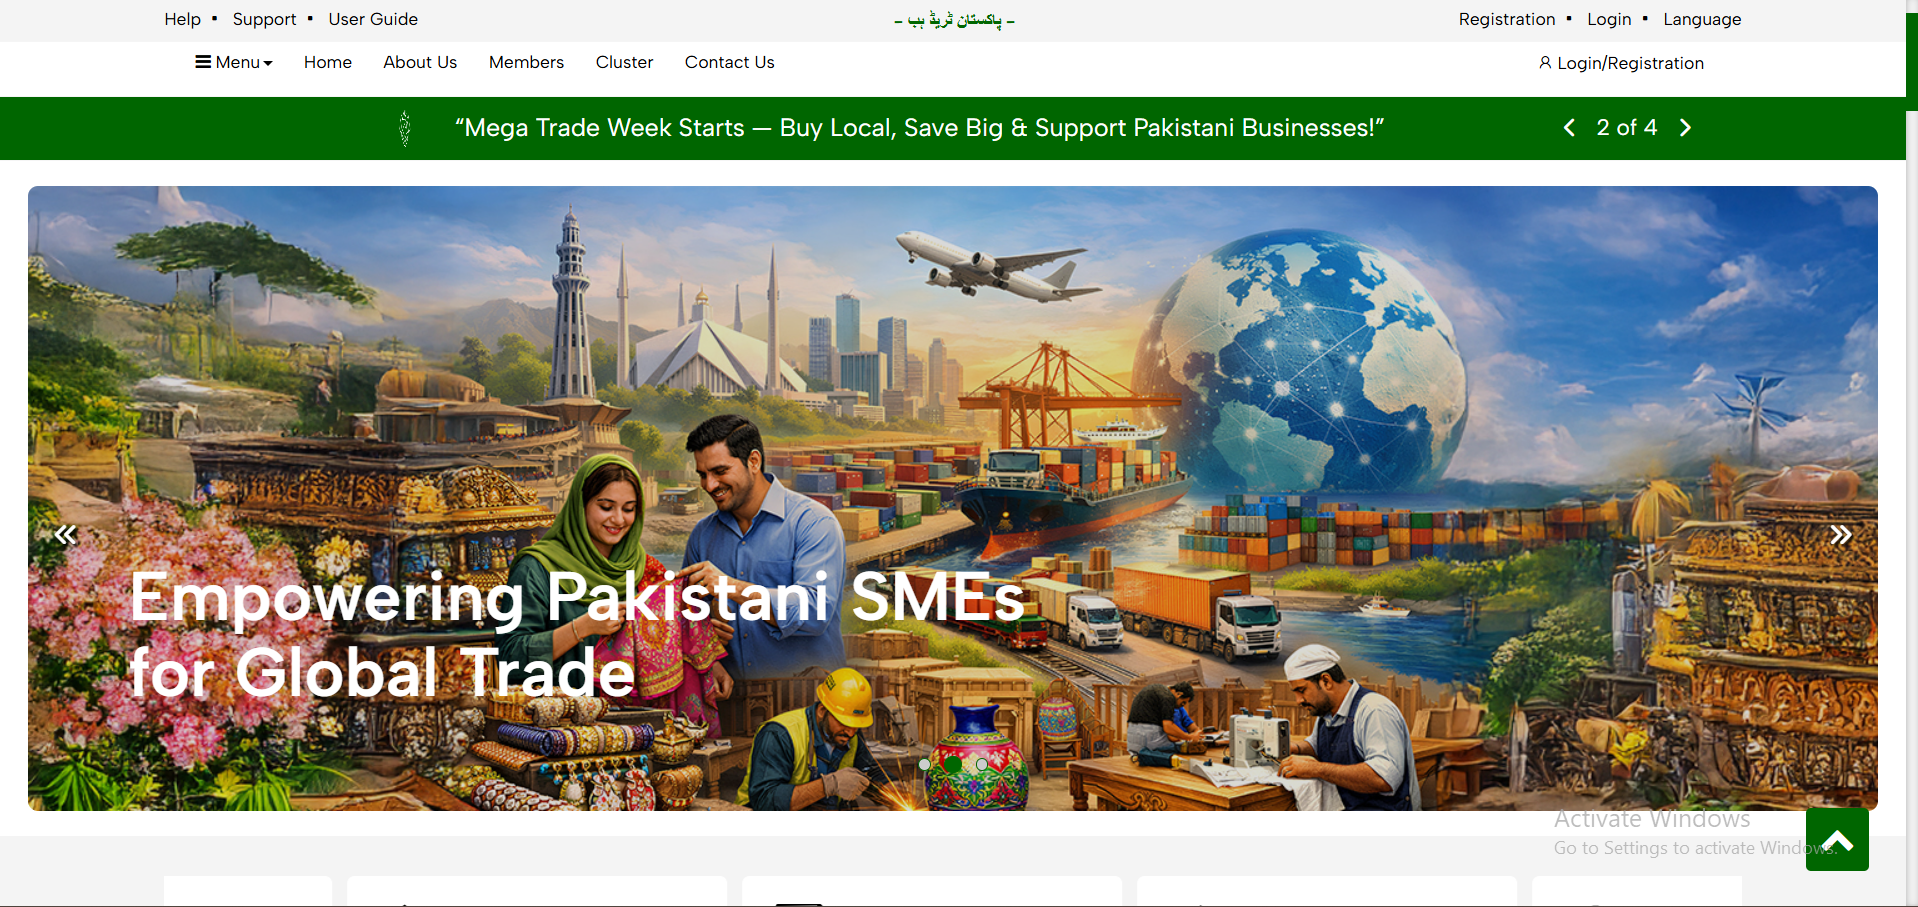
\includegraphics[width=0.92\textwidth]{figures/pictures project/tradehub.png}
    \caption{TradeHub Pakistan Home Page}
    \label{fig:tradehub_pakistan}
\end{figure}

\textbf{Key Features:}
\begin{itemize}
    \item Web-based platform, desktop-first design.
    \item Product catalog including keyword search.
    \item Email notification and inquiry system.
    \item Basic seller ratings
    \item Manual invoice and payment system.
    \item Weak support of Urdu language.
\end{itemize}

\textbf{Limitations:}
Although TradeHub Pakistan enjoys a market presence, it is faced with a number of important constraints \cite{ali2022ecommerce}. The desktop-centered design limits access by the mobile users in the remote regions. The email based communication system causes delays in the negotiation process and sometimes it takes 24-48 hours to reply. The platform does not have real-time notifications, which restrict buyer interaction and responsiveness to the market. There is manual payment processing, which poses security risks and decreases the effectiveness of transactions. The poor multilingual support is frustrating to Urdu speaking users who form a large market segment in Pakistan.

\subsection{System 2: BulkExchange}

BulkExchange is a B2B application created in 2021 that focuses on bulk orders and group buying (all mobile-based). The platform is connected to various local payment gateways, and it has tiered bulk pricing. Communication capabilities, however, are restricted to a bare-bones messaging application without the ability to communicate in real-time.

\begin{figure}[H]
    \centering
    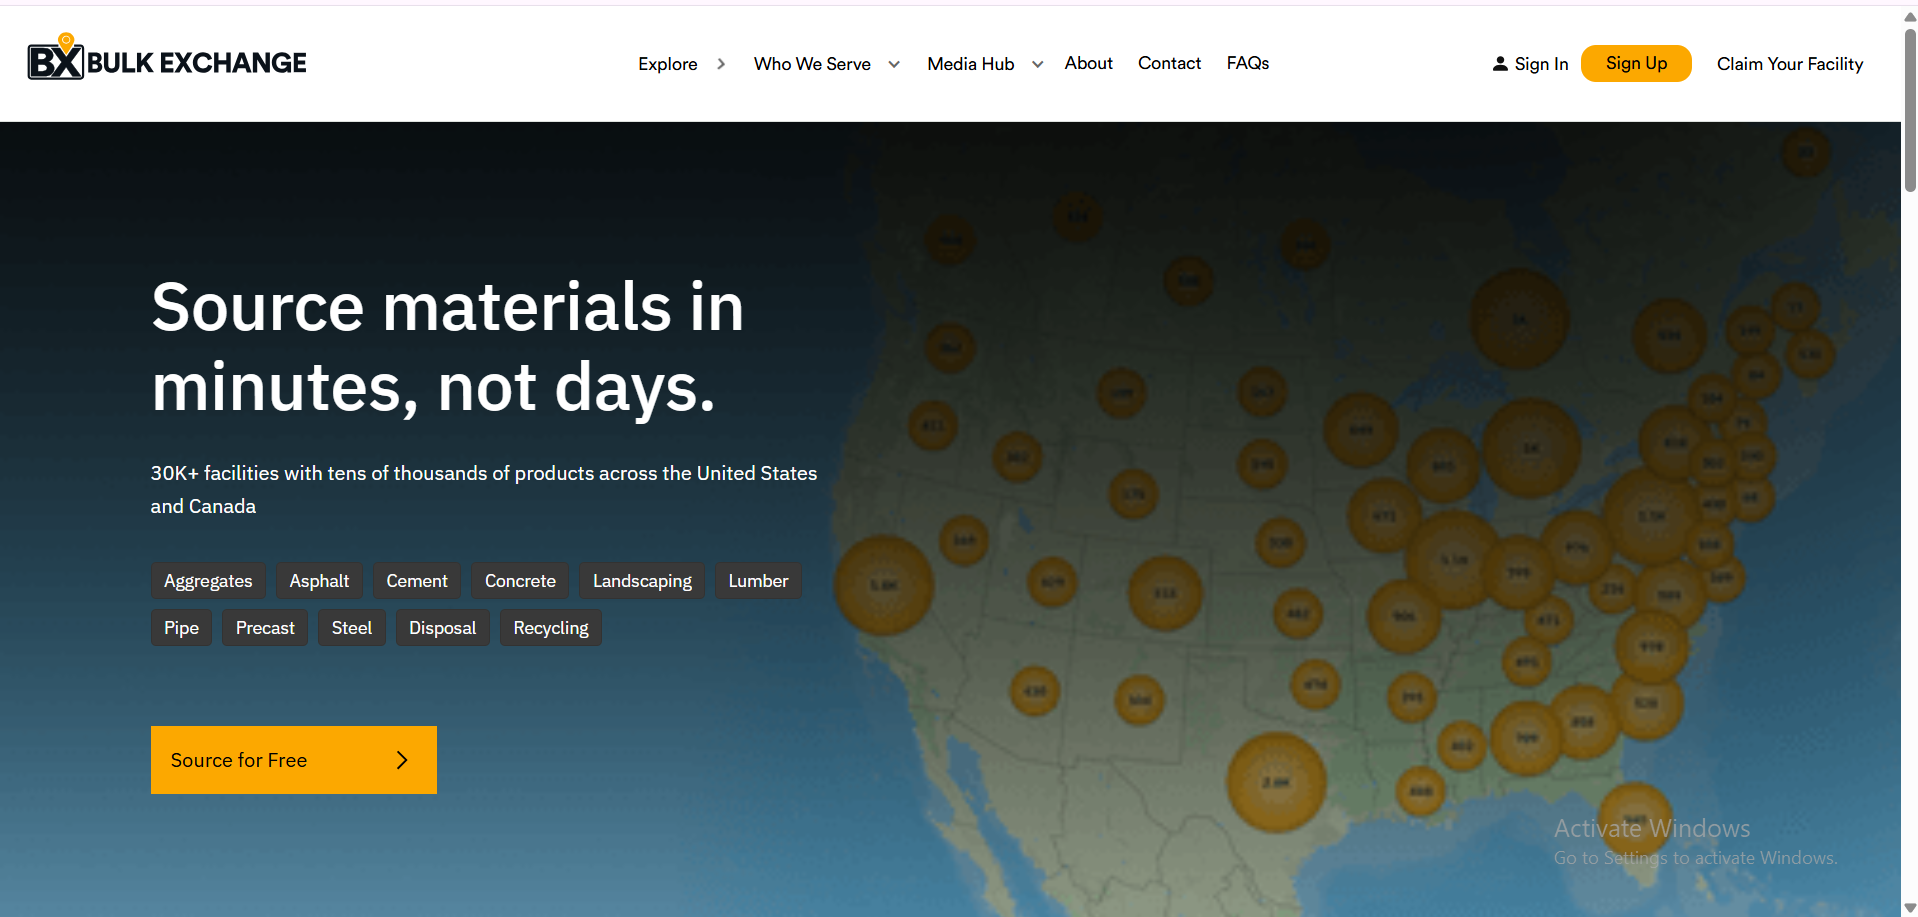
\includegraphics[width=0.92\textwidth]{figures/pictures project/bulkexchange.png}
    \caption{BulkExchange Home Page}
    \label{fig:bulkexchange_home}
\end{figure}

\textbf{Key Features:}
\begin{itemize}
    \item iOS and Android mobile application.
    \item Tiered pricing on bulk orders.
    \item Support of chosen payment gateways.
    \item Simple in-app chat functionality.y
    \item Order tracking system.
    \item Support of only one language (English only)
\end{itemize}

\textbf{Limitations:}
Although BulkExchange focuses on the mobile accessibility, it has significant weaknesses \cite{farooq2024mobile}. The chat feature uses a delayed message queue mechanism instead of a real-time communication mechanism so that there are communication delays that prevent price negotiations. The platform does not have AI-enabled functions to review products or learn more about the market needs, so it is hard to have sellers enhance their offerings based on the feedback of buyers. There is no RFQ (Request for Quotation) system, which restricts the possibilities of buyers to request competitive bids.

\subsection{System 3: PakWholesale}

PakWholesale is a regional wholesale marketplace established in 2020, partnering with major logistics providers to offer integrated supply chain solutions. The platform emphasizes inventory management and shipping integration but has weak communication and transaction support \cite{hussain2023supply}.

\begin{figure}[H]
    \centering
    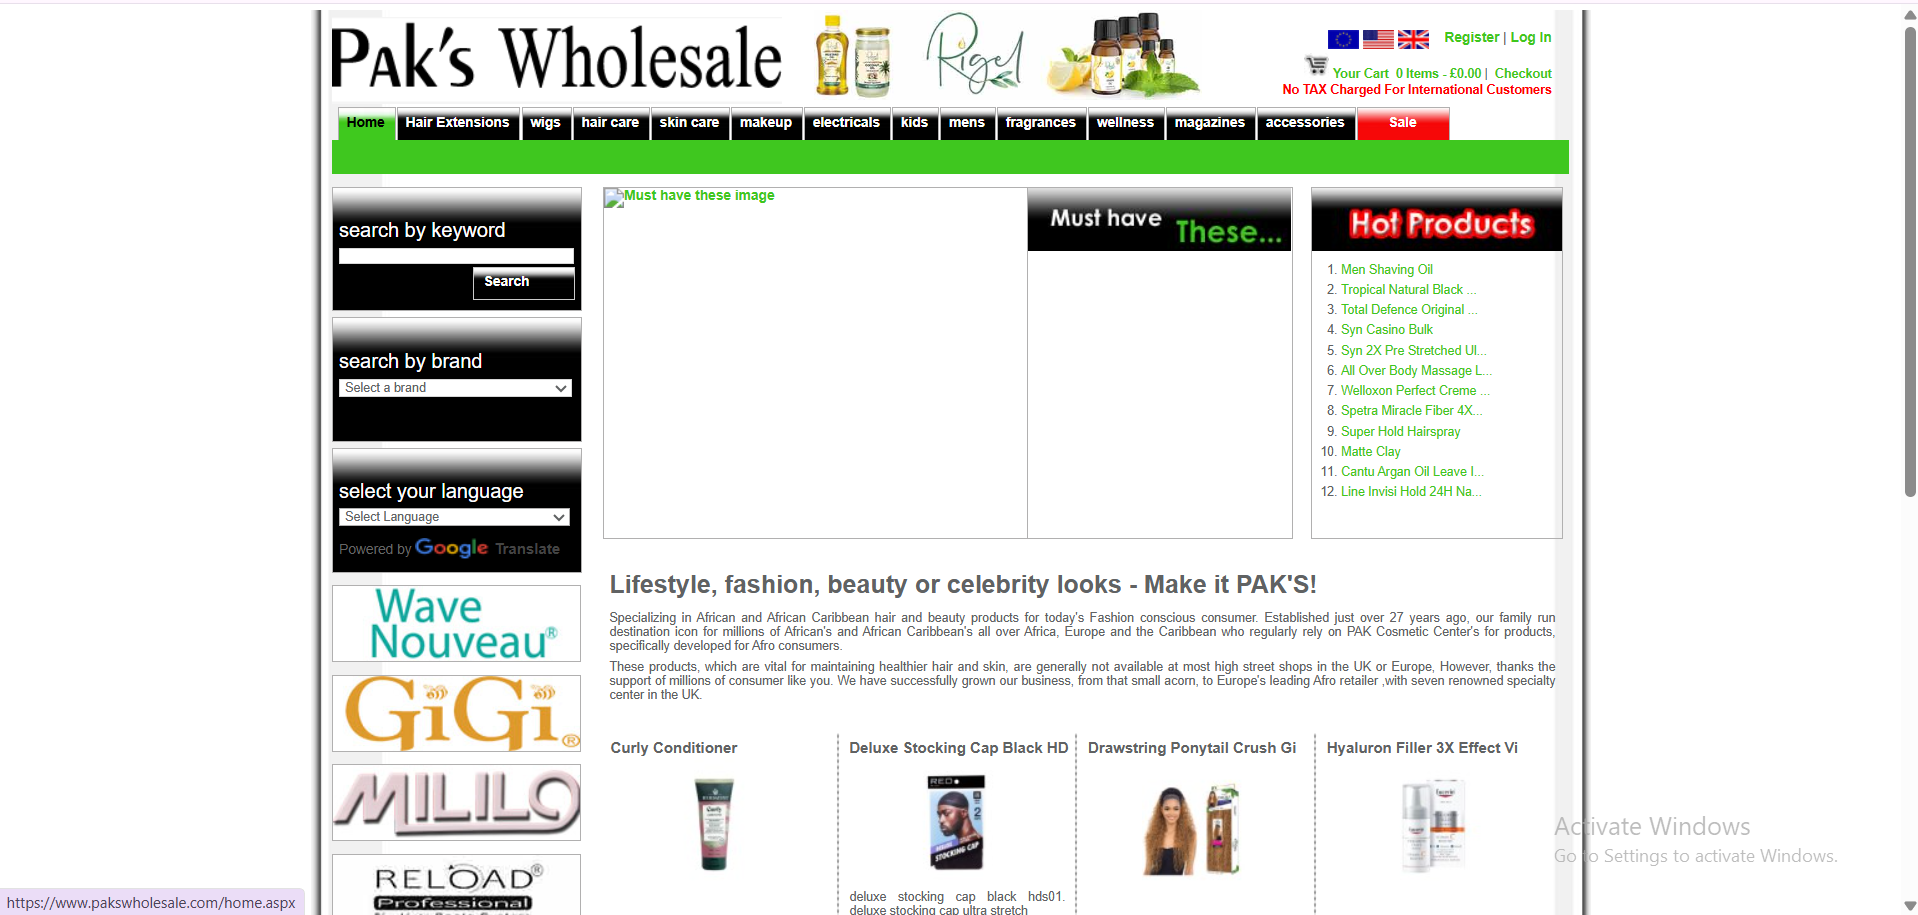
\includegraphics[width=0.92\textwidth]{figures/pictures project/pakwholesales.png}
    \caption{PakWholesale Home Page}
    \label{fig:pakwholesale_home}
\end{figure}

\textbf{Key Features:}
\begin{itemize}
    \item Integration with national logistics providers
    \item Inventory management dashboard for sellers
    \item Automated shipping quote generation
    \item Standardized product categories
    \item Limited product review system
    \item Two-factor authentication for security
\end{itemize}

\textbf{Limitations:}
Despite its logistics integration, PakWholesale demonstrates significant gaps in user engagement \cite{shaikh2024design}. Direct communication between buyers and sellers is restricted, forcing all inquiries through an intermediary support team, which creates unnecessary delays and reduces negotiation flexibility. The platform lacks AI-based insights, providing no automated summaries of customer feedback to help sellers understand buyer preferences. No real-time notifications exist for order status updates or chat messages, reducing transparency for both parties. The payment system relies on institutional bank transfers, excluding smaller enterprises without formal banking infrastructure.

\vspace{1em}

\section{Comparative Analysis: Why Indus Bazar is Superior}

This section compares Indus Bazar against the three existing systems across critical dimensions of B2B marketplace functionality, demonstrating clear competitive advantages.

\begin{table}[H]
\centering
\caption{Comparative Analysis of B2B Marketplace Platforms}
\label{tab:system_comparison}
\renewcommand{\arraystretch}{1.4}
\footnotesize
\begin{tabular}{|>{\raggedright}p{2.8cm}|>{\raggedright}p{2cm}|>{\raggedright}p{2cm}|>{\raggedright}p{2cm}|>{\raggedright\arraybackslash}p{2.2cm}|}
\hline
\rowcolor{lightgray}
\textbf{Feature/Capability} & \textbf{TradeHub Pakistan} & \textbf{BulkExchange} & \textbf{PakWholesale} & \textbf{Indus Bazar} \\
\hline

Mobile-First Architecture & No (Web-based) & Yes (Basic) & Partial & Yes (Flutter) \\
\hline

Real-Time Chat & Email-based & Delayed queue & Restricted & Real-time messaging \\
\hline

Bilingual Support (English/Urdu) & Limited Urdu & English only & English only & Full bilingual \\
\hline

AI-Powered Features & None & None & None & Review summarization \\
\hline

Secure Payment Integration & Manual & Selected gateways & Bank transfer & Stripe integration \\
\hline

Push Notifications & Email only & Limited & None & Real-time Firebase \\
\hline

RFQ Marketplace & No & No & No & Yes \\
\hline

Tiered Bulk Pricing & Manual & Yes & Yes & Advanced automation \\
\hline

Seller Dashboard & Basic & Limited & Inventory-focused & Comprehensive \\
\hline

User Authentication & Basic & Standard & Standard & Multi-role with email verification \\
\hline

Design Philosophy & Enterprise-heavy & Consumer-focused & Logistics-focused & Business-user-centric \\
\hline

Market Focus & Pakistan & Pakistan/India & Pakistan & Pakistan (Regional potential) \\
\hline

\end{tabular}
\end{table}

\subsection{Mobile-First and Accessible Architecture}

Indus Bazar is built entirely on Flutter, ensuring cross-platform compatibility and superior performance on Android and iOS devices. Unlike TradeHub Pakistan's desktop-centric approach, Indus Bazar prioritizes mobile accessibility, enabling business users in remote areas without reliable desktop infrastructure to participate in the marketplace \cite{farooq2024mobile}. The responsive design with intuitive navigation reduces the learning curve compared to BulkExchange's basic mobile interface.

\subsection{Real-Time Communication and Negotiation}

The integrated real-time chat system in Indus Bazar enables instant communication between buyers and sellers, fundamentally accelerating negotiation cycles. TradeHub Pakistan's email-based system creates 24-48 hour delays, while BulkExchange's delayed message queue introduces latency. PakWholesale's intermediary-based system adds friction to direct negotiations. Indus Bazar's WebSocket-based real-time messaging supports immediate price discussions, clarifications, and relationship building \cite{ali2022ecommerce}, critical for B2B trust development.

\subsection{Bilingual and Culturally Appropriate Design}

Indus Bazar's comprehensive bilingual support (English and Urdu) addresses a major gap in existing platforms. All three competitors either lack Urdu support entirely or provide minimal translation. Research by Akram and Latif (2022) \cite{akram2022user} demonstrates that multilingual interfaces increase adoption by 35\%. Indus Bazar's design considers local business practices, cultural preferences, and familiar communication patterns, creating a more welcoming environment for Pakistani wholesalers and retailers.

\subsection{AI-Driven Insights and Review Summarization}

Indus Bazar uniquely incorporates AI-powered review summarization, generating concise insights from customer feedback in both English and Urdu. This capability is absent from all three existing systems, providing sellers with actionable intelligence to improve products and services. The AI component helps sellers understand buyer preferences quickly without reading lengthy reviews \cite{hussain2023supply}, enabling data-driven product development and market responsiveness.

\subsection{Advanced Payment Security and Flexibility}

Through Stripe integration with test mode functionality, Indus Bazar provides secure, PCI-compliant payment processing with fraud protection mechanisms. TradeHub Pakistan's manual payment handling creates security vulnerabilities. BulkExchange's limited gateway integration and PakWholesale's institutional bank transfer requirement exclude informal businesses and small enterprises \cite{zafar2022trust}. Indus Bazar's flexible payment approach serves the entire business spectrum in Pakistan.

\subsection{Comprehensive Push Notification System}

Indus Bazar leverages Firebase and Appwrite for real-time notifications, immediately alerting users to order updates, chat messages, and system activities. TradeHub Pakistan relies on email, and PakWholesale lacks notifications entirely. Timely notifications reduce order fulfillment delays and enhance user engagement, critical factors for marketplace stickiness and market efficiency.

\subsection{Request for Quotation (RFQ) Marketplace}

The RFQ functionality in Indus Bazar enables buyers to post product requests and receive competitive bids from multiple sellers simultaneously. This feature is absent from all three competitors, providing Indus Bazar with a distinctive mechanism for price discovery, buyer empowerment, and competitive market dynamics. The RFQ system reduces buyer search costs and enables sellers to compete on quality and pricing \cite{raza2023impact}.

\subsection{Role-Based Access Control and Security}

Indus Bazar implements multi-role access control differentiating manufacturers, wholesalers, retailers, and customers with appropriate permission scopes. This granular security framework exceeds the basic authentication in existing systems. Email verification and password recovery via secure deep linking ensure account security while maintaining user experience quality. Role-based access enables each user type to access only relevant features and data \cite{porter2001strategy}, improving both security and interface clarity.

\vspace{2em}

\section{Summary of Competitive Advantages}

Indus Bazar addresses critical gaps in the existing B2B marketplace landscape in Pakistan:

\begin{itemize}
    \item \textbf{Holistic Feature Integration:} Unlike competitors focusing on single dimensions (logistics, bulk pricing, or chat), Indus Bazar integrates comprehensive capabilities—communication, payments, AI insights, and notifications—in a unified platform.
    
    \item \textbf{Cultural and Linguistic Alignment:} Full bilingual support and culturally appropriate design significantly reduce friction for local business users compared to English-only platforms.
    
    \item \textbf{Mobile-centric Architecture:} Flutter-based development enables accessing underserved rural markets and businesses without desktop infrastructure, expanding addressable market potential.
    
    \item \textbf{Advanced Functionality:} AI review summarization and RFQ marketplace features provide capabilities unavailable in existing systems, enhancing market transparency and efficiency.
    
    \item \textbf{Security and Trust:} Secure payment integration, multi-role access control, and email verification build business confidence critical for B2B adoption.
    
    \item \textbf{Real-Time Engagement:} Real-time chat, push notifications, and instant RFQ mechanics reduce transaction cycle times and create dynamic market conditions compared to asynchronous systems.
\end{itemize}

By combining technological sophistication with deep understanding of Pakistani business practices, Indus Bazar is positioned to becoming the preferred B2B marketplace for manufacturers, wholesalers, and retailers seeking efficient, secure, and culturally aligned commerce in Pakistan's digital economy.






\chapter{Requirement Specifications} \label{chap:reqs}

%\version{v1.10.2015}

\section*{}
\section{Existing System}
The wholesale and bulk trading industry in Pakistan has been traditionally relying on middlemen, personal contacts, and face-to-face communication. There have been a number of digital B2B platforms developed to fill this gap, such as Alibaba, IndiaMart, TradeKey Pakistan and local classifieds like OLX and PakWholesalers. The purpose of these platforms is to match buyers and sellers on a digital platform, yet they cannot meet the needs of the small and medium enterprise (SME) sector of Pakistan specifically \cite{ali2022ecommerce}. The majority of these platforms are either too generic to conduct local business or offer functionalities that are too few to facilitate efficient bulk trade and direct business negotiations \cite{hussain2023supply}.

\subsection{Limitations of the Existing System}
The already existing B2B platforms, though useful in a number of ways, have grave shortcomings in terms of catering to the unique needs of Pakistani manufacturers, wholesalers, and retailers:

\begin{itemize}
    \item The absence of real-time communication between buyers and sellers and, therefore, slow and inefficient negotiations.
    \item Lack of multilingual assistance (especially Urdu), restricting access to local businesses \cite{akram2022user}.
    \item Lack of an built-in Request for Quotation (RFQ) system to negotiate custom bulk-orders.
    \item No tiered or bulk pricing models to support wholesale transactions.
    \item  Interfaces that are complicated enough to be inaccessible to small sellers or too simple to allow growing businesses to develop further \cite{han2023digital}.
    \item Lack of mobile optimization and thus poor user experiences on smartphones.
    \item No AI assisted product review analysis or market knowledge.
    \item Absence of push notification systems to give prompt order and communication notices.
    \item Overdependence on intermediaries, rising costs, decreasing transparency of the supply chain \cite{raza2023impact}.
\end{itemize}

\section{Proposed System}
Indus Bazar is a mobile based B2B marketplace application, which aims to directly integrate manufacturers, wholesalers, and retailers in a single digital platform. The system offers an all-inclusive collection of applications that allows business to find products, negotiate bulk purchases, make transactions, and communicate in real time, all in one application \cite{farooq2024mobile}. The platform was developed with Flutter, Dart, and Appwrite, supporting both Urdu and English, which will provide the appropriate cultural alignment and allow Pakistani users to use it. Indus Bazar combines artificial intelligence-driven review summarization, secure Stripe payment processing, a Request for Quotation (RFQ) marketplace, tiered bulk pricing, and chat to provide a seamless, transparent and efficient B2B commerce experience.

\subsection{The Proposed System Overcomes the Limitations of the Existing Systems.}
the Limitations of the Existing Systems.
To directly overcome the limitations of the current systems, the following innovative features are applied by Indus Bazar:

\begin{itemize}
    \item Will offer a live chat platform that will allow buyers and sellers to communicate instantly and negotiate directly.
    \item Provides support of Urdu and English interface to provide accessibility and cultural suitability to Pakistani users \cite{akram2022user}.
    \item It has an exclusive RFQ (Request for Quotation) Marketplace, where a customer can post requests on items, and sellers compete to offer the best price.
    \item Adopts the levels of pricing to facilitate bulk buying with automatic price discounts according to the order quantity.
    \item Provides a mobile-first, easy to use, user-friendly interface that works well with Android devices and is scalable to businesses of any size \cite{farooq2024mobile}.
    \item Incorporates AI-enhanced review summarization to enable buyers to make a wise choice and aid sellers in gaining insight into customer feedbacks \cite{chaffey2022digital}.
    \item Supports push notifications to deliver timely order, chat, and system updates.
    \item Minimizes the need to intermediaries by allowing direct digital links between both manufacturers and buyers, decreasing expenses and enhancing transparency \cite{hussain2023supply}.
\end{itemize}

\section{Requirements Specifications}
System requirements are divided into functional and non-functional requirements for an optimum and user-friendly platform. Functional requirements refer to the set of features and functionalities that the system should possess in order to address the needs of customers and sellers in the Indus Bazar marketplace. Non-functional requirements focus on system quality, security and performance issues to address the needs of system usability.  The functional and non-functional requirements are necessary to develop the Indus Bazar as a secure, scalable and accessible B2B marketplace for Pakistan‘s digital economy.

\section{Functional Requirements}
Functional requirements: define the essential functions provided by the Indus Bazar platform to enable complete B2B commerce functionality. These requirements dictate the expected system behaviour for the customer-side functionality (such as login,  browse and select products,  place purchase orders,  and payment) and seller-side functionality (such as login,  add/edit/remove products,  and balance invoice requests); and include the RFQ marketplace,  turn-based communication, and notification services.  Every functional requirement can be traceably linked to use cases that have been identified during the analysis phase,  and can be linked to a testable functionality that must be developed prior to deployment.

\subsection{Login and Registration}
\begin{itemize}
    \item Customers and sellers can register their name, email address, and secure password in the system using a registration form and choose their role (Customer or Seller).
    
    \item When a user registers, a verification email is sent to the provided email address. The user is allowed to access the system only after verifying the email by clicking a deep link.
    
    \item Registered users can log into the system using their email and password. Upon successful authentication, role-based access is provided to either the customer or seller dashboard.
    
    \item The system includes a password recovery option that uses the registered email, allowing users to reset their credentials securely.
    
    \item Role-Based Access Control (RBAC) is implemented to ensure that customers and sellers can only access functions and information relevant to their roles.
\end{itemize}

\subsection{Product Catalog Management}
\begin{itemize}
    \item The system offers a tabular product listing with categories and subcategories, including product descriptions, specifications, and prices.
    
    \item The search engine allows users to find products using keywords, filters (category, price range, and seller), and sorting options to efficiently identify the desired products.
    
    \item Tiered pricing information is displayed in each product listing, with clear per-unit pricing at various order quantity levels.
    
    \item Sellers can add, edit, and delete items in their listings via the seller dashboard, and updates are immediately reflected in the catalog.
    
    \item The system supports multilingual product names and descriptions in both English and Urdu to enhance accessibility.
\end{itemize}

\subsection{Shopping Cart and Checkout}
\begin{itemize}
    \item Shoppers can add or remove items from the shopping cart and modify item quantities before proceeding to checkout.
    
    \item The system automatically calculates the tiered price based on the selected quantity of each product.
    
    \item During checkout, customers can select an existing delivery address or add a new one and confirm the final order summary.
    
    \item The checkout process is streamlined and validated to prevent incomplete or incorrect order submissions.
    
    \item Customers can manage multiple delivery addresses and assign a default address for faster checkout.
\end{itemize}

\subsection{Secure Payment Integration}
\begin{itemize}
    \item The system has been built to connect with Stripe as the payment gateway to enable safe online payments. It is still in test as to confirm the payment workflow.
    
    \item The server-side Appwrite functions are used to process payment to make sure that payment information is never sent to the client-side in an exposed form.
    
    \item It will accept card payments and give real-time payment confirmation or failure messages.
    
    \item The order is automatically created and a push notification sent to the seller associated with the order when it is successfully paid.
    
    \item The records of transactions are well-protected and are accessible to clients and merchants via order histories.
\end{itemize}

\subsection{Order Management}
\begin{itemize}
    \item The system handles all order lifecycle, such as order placement, order processing, order dispatch, and order delivery.
    
    \item Customers are able to use their order history dashboard to track the status of their orders.
    
    \item sellers have access to incoming orders, update on order statuses (Confirmed, Processing, Shipped, Delivered or Cancelled) and fulfillment through the seller dashboard.
    
    \item When an order status is updated, customers and sellers get a push notification.
    
    \item The system has a detailed history of order to aid in business record-keeping and resolving disputes.
\end{itemize}

\subsubsection{Tiered Pricing and Bulk Ordering}
The system also has a tiered pricing model to promote bulk buying. The unit cost reduces with the quantity of order, thus appealing to the retailers and wholesalers to purchase in large quantities. The following table is an example of a tiered pricing structure:

\renewcommand{\arraystretch}{1.2}
\begin{longtable}{|l|l|l|}
\caption{Tiered Pricing Structure Example}\label{tab:tiered_pricing}\\
\hline
\rowcolor{lightgray}
\textbf{Tier} & \textbf{Minimum Order Quantity} & \textbf{Price Per Unit}\\
\hline
\endhead
Tier 1 (Base) & 1+ units & PKR 1,000 per unit\\
\hline
Tier 2 (Wholesale) & 50+ units & PKR 850 per unit\\
\hline
Tier 3 (Bulk) & 100+ units & PKR 700 per unit\\
\hline
\end{longtable}
\renewcommand{\arraystretch}{1}


The tiered pricing model allows sellers to establish a fixed price level of a product, up to three, each having a limited order quantity and a unit price. The price tier to be applied is automatically calculated by the system depending on the amount of units the customer chooses, the higher the units the cheaper the unit price.

The product detail page shows all the pricing levels. Before adding products to their cart, customers have the chance to change the quantity to take advantage of discounted prices. In case of a large order or a tailored order, customers are welcome to negotiate the price directly with the sellers using the RFQ Marketplace.

\subsection{Real-Time Chat System}
\begin{itemize}
    \item The system has a real-time chat option that allows direct customer-seller communication.
    
    \item Text and image messaging is enabled and sellers can share product photos, catalogues, and documents with buyers.
    
    \item Conversations are user specific, and are continuously archived, allowing users to re-examine previous conversations.
    
    \item Push messages inform users immediately about new messages, which helps to respond quickly and negotiate faster.
    
    \item There is chat functionality on both product listing and order page where it can easily be used to communicate.
\end{itemize}

\subsection{RFQ (Request for Quotation) Marketplace}
\begin{itemize}
    \item The system has a dedicated RFQ Marketplace where customers can make requests concerning the items they need such as product name, category, quantity, delivery city, delivery date, optional price range (minimum and maximum) and other specifications.
    
    \item RFQ listings are open to seller quotes of a period up to seven days, and will automatically expire unless a quote is accepted.
    
    \item Sellers are able to see active RFQs and place competitive bids with unit price and total price, expected time of delivery and notes.
    
    \item Push messages are delivered to the customers every time a new quote is offered, and the customers can review, compare and accept the most appropriate offer.
    
    \item Accepted quotations are automatically turned into order to be checked out with the agreed price applied, and competing quotations are rejected.
    
    \item RFQ option will remove the necessity of any external communication channels and provide clear, well-documented trade negotiations inside the platform.
\end{itemize}

\subsection{AI-Powered Review Summarization}
\begin{itemize}
    \item The system has an AI-powered module which analyzes reviews of customers of specific products and creates readable short summary on-demand.
    
    \item Summaries are initiated by the user. On clicking the \textit{Generate Summary} button on the product detail page, an Appwrite cloud functions produces the summary in the chosen language.
    
    \item Summaries come in both Urdu and English. The product detail page has a toggle option which enables the user to use alternative languages without re-generating the summary.
    
    \item Reviews are only allowed to people who have made confirmed purchases of the product i.e. people who have placed non-refunded orders and the product received.
    
    \item AI-generated summaries enable sellers to swiftly comprehend customer sentiment in general, and areas of product or service enhancement.
    
    \item The AI part of the platform can only review summarization in the current version.
\end{itemize}

\subsection{Push Notifications}
\begin{itemize}
    \item The system provides real-time push notifications of crucial events like order placements, status updates, chat messages, and RFQ related events.
    
    \item Firebase Cloud Messaging (FCM) and Appwrite messaging services are used to implement the notifications.
    
    \item Customers and sellers get role specific notifications to keep them posted on their activities on the platform.
    
    \item The app has an option of viewing the history of notification in the future.
    
    \item The notification system works when the application is not in the background or after closing the application.
\end{itemize}

\subsection{Report Generation}
\begin{itemize}
    \item Order History: The users can get a full view of their order history including the order dates, products, quantities, totals and the statuses.
    
    \item Transaction Records: Views all financial transactions by customers or to sellers, including Stripe transaction IDs and times.
    
    \item Seller Sales Overview: Sellers will have access to aggregate sale information, such as fulfilled orders, total revenue, and products sold most.
    
    \item RFQ Activity: Tracks the submitted quotes, accepted deals, pending negotiations by the sellers and the submitted requests by the customers.
    
    \item{Review Analytics: The product performance of the sellers can be tracked using AI-generated summaries of reviews and customer feedback in a single dashboard.
\end{itemize}

\subsection{Administrative Functions}
\begin{itemize}
    \item Seller Dashboard: Sellers can use a special dashboard where they can see an overview of active posts, orders, active chat, and quotes.
    \item Product Management: Sellers are able to add and update their listings, control pricing levels, and delete discontinued products.
    \item Order Fulfillment Control: Sellers can change the status of orders at all points throughout the fulfillment lifecycle and attach tracking or delivery notes.
    \item Quote Management: Sellers are able to handle all quoted items, monitor accepted and pending RFQ requests, and respond to customer requests.
    \item Performance Monitoring: AI-generated summary of reviews and order statistics can help sellers track product performance and customer feedback to optimize their offerings.
\end{itemize}

\section{Non-Functional Requirements}
\begin{itemize}
    \item \textbf{Security:} The system should be equipped with strong authentication, role-based access control, email authentication, and secure server-side payment processing to secure user accounts and sensitive business data.
    
    \item \textbf{Performance:} The site should be able to provide quick load times, chat responsiveness in real time, and timely push notifications to have an efficient user experience on all core functionality.
    
    \item Scalability The system should have the ability to handle an increasing number of simultaneous users, product entries, and transactions without affecting its performance negatively (Laudon 2023ecommerce).
    
    \item Availability: The platform should be highly available to guarantee that users can access the marketplace, manage orders and communicate any time.
    
    \item \textbf{Usability:} The interface needs to be simple and user-friendly to both small and large business with a mobile-first design that is Android-friendly.
    
    \item Multilingual Support: The system should be bilingual in Urdu and English, covering both main interface elements and the content of the products and AI-generated summaries to address the needs of the diverse Pakistani market.
    
    \item Data Privacy and Compliance: The system should guarantee the privacy of user data, business data and transaction records by deploying proper encryption and access control.
\end{itemize}

\section{User Requirements}
\begin{itemize}
    \item \textbf{Customer Registration and Login.}
    \begin{itemize}
        \item The ability to create an account including name, email, password, and role choice (Customer or Seller).
        \item Before accessing the platform email validation is to be done.
        \item protected log-in and access to a role-based, personalized dashboard.
        \item Recovery of passwords through registered email.
    \end{itemize}

    \item \textbf{Product Discovery}
    \begin{itemize}
        \item The ability to navigate a structured product catalog in categories and subcategories.
        \item Advanced search and filtering features in order to find certain products fast.
        \item Tiered pricing information on the product detail page.
        \item Read AI-generated review summaries in English or Urdu to make an informed purchase.
    \end{itemize}

    \item \textbf{Shopping Cart and Checkout.}
    \begin{itemize}
        \item Add products to a cart, change quantities, and preview prior to checking out.
        \item Add more than one address to be used when making a delivery.
        \item Simplified checkout experience and automatic calculation of price tiers.
    \end{itemize}

    \item \textbf{Payment and Order Management.}
    \begin{itemize}
        \item Card-based payment processing using Stripe with real-time confirmation.
        \item Full order history with tracking of status, starting with placement through delivery.
        \item Push notifications of all changes of order status.
    \end{itemize}

    \item \textbf{RFQ and Negotiation.}
    \begin{itemize}
        \item Capacity to post RFQ requests including product requirements and specifications.
        \item Review and compare quotes posted by several sellers.
        \item Accept desired quote and go straight to checkout at agreed price.
    \end{itemize}

    \item \textbf{Real-Time Communication}
    \begin{itemize}
        \item Face to face negotiation, communication, and clarification with the sellers.
        \item Text and image message support in chat interface.
        \item Real time push notifications of new messages.
    \end{itemize}

    \item \textbf{Seller Registration and Dashboard.}
    \begin{itemize}
        \item Sellers will have the opportunity to register, verify their email and get a dedicated seller dashboard.
        \item Product listing product listing and product listing additions/updates/removals with tiered pricing.
        \item See and complete incoming customer orders with status update features.
        \item Respond to RFQ requests by customers.
        \item observe the performance of products with a review summary and sales report.
    \end{itemize}

    \item \textbf{Multilingual Accessibility}
    \begin{itemize}
        \item Platform interface and AI-generated summaries (both English and Urdu).
        \item Simple, interactive design that can be used by various users in Pakistan.
    \end{itemize}

    \item \textbf{Availability}
    \begin{itemize}
        \item Platform available 24/7 to facilitate business operations and time sensitive transactions.
    \end{itemize}
\end{itemize}

\section{Use Case Diagram}

In this section, the UML Use Case Diagrams of the Indus Bazar B2B Marketplace Application will be provided and the key interactions between the system and the two main actors, the Customer and the Seller in the core functional areas of the system.

\subsection{Customer System Use Case}
The Customer System Use Case diagram below shows the entire list of interactions that a customer is able to achieve on the Indus Bazar platform, such as authentication, product-finding, purchasing, and bargaining processes.

\begin{figure}[H]
\centering
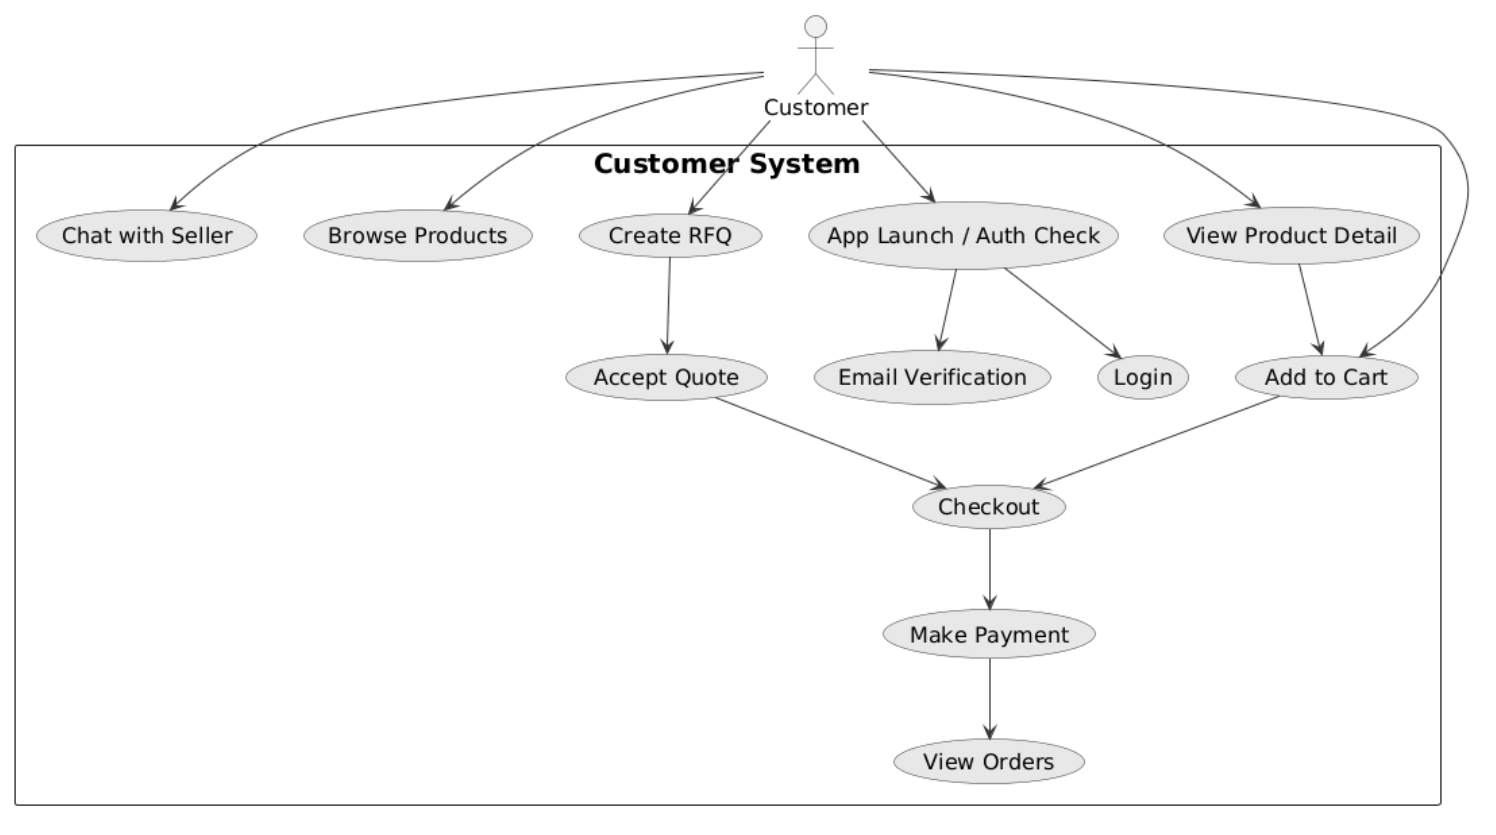
\includegraphics[width=0.95\textwidth]{figures/pictures project/customer_usecase.png}
\caption{Customer System Use Case Diagram}
\label{fig:customer_use_case_diagram}
\end{figure}

The use case diagram shown in Figure \ref{fig:customer_use_case_diagram} demonstrates all the possible interactions that the Customer actor can have in the Indus Bazar system. The diagram illustrates:

\begin{itemize}
    \item \textbf{Primary Actor:} Customer communicating with all core purchasing and communication functions.

    \item \textbf{Authentication Flow:}
    \begin{itemize}
        \item App Launch / Auth Check - system checks whether the user has already been authenticated on launch.
        \item Login - Customer enters the credentials to enter the platform.
        \item Email Verification - after initial registration, they need to go through the email verification.
    \end{itemize}

    \item \textbf{Core Use Cases:}
    \begin{itemize}
        \item Browse Products — customer browses products catalog.
        \item View Product Detail Customer sees detailed product information and tiered pricing.
        \item Develop RFQ customer makes a request of quotation of bulk or custom orders.
        \item Chat with Seller — customer is in direct communication with a seller.
        \item Accept Quote - customer reviews the quote that has been submitted by a seller and accepts it.
        \item Add to Cart — customer will add items to the shopping cart.
        \item Checkout Customer reviews cart and selects address to deliver to and confirms order.
        \item Make Payment - customer makes the payment using Stripe.
        \item View Orders — customer follows orders placed and order history.
    \end{itemize}
\end{itemize}

\subsection{Seller System Use Case}

The Seller System Use Case diagram below displays the interaction that can be offered to a seller on the Indus Bazar platform and includes the activities of authentication, product management, order fulfillment, and interaction with customers.

\begin{figure}[H]
\centering
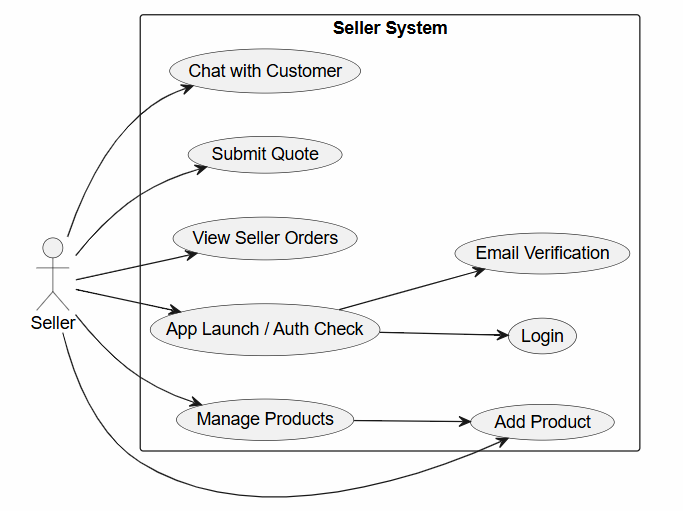
\includegraphics[width=0.85\textwidth]{figures/pictures project/seller_usecase.png}
\caption{Seller System Use Case Diagram}
\label{fig:seller_use_case_diagram}
\end{figure}

The use case diagram shown in Figure \ref{fig:seller_use_case_diagram} illustrates the seller-side interactions within the Indus Bazar system. The diagram illustrates:

\begin{itemize}
    \item \textbf{Primary Actor:} Seller managing products, orders, quotes, and customer communication.

    \item \textbf{Authentication Flow:}
    \begin{itemize}
        \item App Launch / Auth Check — system verifies seller session status on launch
        \item Login — seller authenticates to access the seller dashboard
        \item Email Verification — mandatory on registration for seller account activation
    \end{itemize}

    \item \textbf{Core Use Cases:}
    \begin{itemize}
        \item Manage Products — seller manages the full lifecycle of product listings
        \item Add Product — seller creates new product listings with pricing tiers and details
        \item Submit Quote — seller responds to customer RFQ requests with competitive offers
        \item View Seller Orders — seller monitors and fulfills incoming customer orders
    \end{itemize}
\end{itemize}

\subsection{Use Case Specifications}

This section gives the important specifications of each of the use cases in the Indus Bazar system, including use case ID, name, actors, preconditions, basic flow, alternative flows, and postconditions, in a tabular form.

\subsubsection{Login}
The use case of login, as illustrated in the table below (Login) \ref{tab:use_case_login} outlines how the registered customers and sellers can securely access the Indus Bazar platform and its services. 
\renewcommand{\arraystretch}{1.3}
\begin{longtable}{|p{3cm}|p{10cm}|}
\caption{Use Case - Login}\label{tab:use_case_login}\\
\hline
\rowcolor{lightgray}
\textbf{Attribute} & \textbf{Description}\\
\hline
\endhead
\textbf{Use Case ID} & UC-01\\
\hline
\textbf{Use Case Name} & Login\\
\hline
\textbf{Actors} & Customer, Seller\\
\hline
\textbf{Description} & Enables registered users to log in securely and access their respective role-based dashboards.\\
\hline
\textbf{Preconditions} & User has a registered and email-verified account.\\
\hline
\textbf{Basic Flow} & 1. User opens the login page.\newline 2. Enters registered email and password.\newline 3. System verifies credentials and determines role.\newline 4. User is redirected to the customer or seller dashboard.\\
\hline
\textbf{Alternative Flows} & Invalid credentials \textrightarrow\ Error message displayed; access denied.\\
\hline
\textbf{Post Conditions} & User is authenticated and directed to the appropriate role-based dashboard.\\
\hline
\textbf{Frequency of Use} & Very Frequent\\
\hline
\textbf{Priority} & High\\
\hline
\end{longtable}

\subsubsection{Registration}
The Registration use case \ref{tab:use_case_registration} enables new customers and sellers to open a new account at the Indus Bazar platform. The system verifies the information given and sends an email verification link through deep link and only after the verification is successful is an access granted. The registration time defines the selection of roles, i.e. the user or seller management dashboard.

\renewcommand{\arraystretch}{1.3}
\begin{longtable}{|p{3cm}|p{10cm}|}
\caption{Use Case - Registration}\label{tab:use_case_registration}\\
\hline
\rowcolor{lightgray}
\textbf{Attribute} & \textbf{Description}\\
\hline
\endhead
\textbf{Use Case ID} & UC-02\\
\hline
\textbf{Use Case Name} & Registration\\
\hline
\textbf{Actors} & Customer, Seller\\
\hline
\textbf{Preconditions} & User does not already have a registered account.\\
\hline
\textbf{Basic Flow} & 1. User opens the registration page.\newline 2. Enters name, email, password, confirm password, and selects role (Customer or Seller).\newline 3. System validates input and creates the account.\newline 4. Verification email is sent to the provided address via deep link.\newline 5. User clicks the verification link and is redirected to login.\\
\hline
\textbf{Alternative Flows} & Email already registered \textrightarrow\ Error message shown.\newline Invalid input format \textrightarrow\ Validation error displayed.\\
\hline
\textbf{Post Conditions} & Account created and email verified; user can now log in.\\
\hline
\textbf{Frequency of Use} & Moderate (once per user)\\
\hline
\textbf{Priority} & High\\
\hline
\end{longtable}

\subsubsection{Browse Products}
The Browse Products use case \ref{tab:use_case_browse_products} enables customer to browse the product offerings of the platform with ease through structured navigation and search features. Users can categorize products, sub categorize them and use the relevant attributes to filter or use key word searches to identify certain products. These inputs are processed by the system and the results that match are retrieved in real time and in a structured and easy to use format. All product listings contain fundamental product data like product name, thumbnail image, seller name and price, which allows a rapid comparison of a variety of products. The system can also be used to facilitate more sophisticated filters like price range, rating or availability to narrow down search results. Where no similar products are located, the system will give useful suggestions or reminders to adjust the search parameters. The use case is crucial in improving product discoverability and overall user experience through making informed decisions.

\renewcommand{\arraystretch}{1.3}
\begin{longtable}{|p{3cm}|p{10cm}|}
\caption{Use Case - Browse Products}\label{tab:use_case_browse_products}\\
\hline
\rowcolor{lightgray}
\textbf{Attribute} & \textbf{Description}\\
\hline
\endhead
\textbf{Use Case ID} & UC-03\\
\hline
\textbf{Use Case Name} & Browse Products\\
\hline
\textbf{Actors} & Customer\\
\hline
\textbf{Description} & Allows customers to search and filter the product catalog to find products meeting their requirements.\\
\hline
\textbf{Preconditions} & Customer is logged in.\\
\hline
\textbf{Basic Flow} & 1. Customer opens the product catalog.\newline 2. Applies category filters or enters search keywords.\newline 3. System displays matching products with thumbnail, price, and seller information.\\
\hline
\textbf{Alternative Flows} & No results found \textrightarrow\ System displays a message suggesting alternative search terms.\\
\hline
\textbf{Post Conditions} & Customer views a filtered list of products matching the search criteria.\\
\hline
\textbf{Frequency of Use} & Very Frequent\\
\hline
\textbf{Priority} & High\\
\hline
\end{longtable}

\subsubsection{View Product Detail}
The View Product Detail use case \ref{tab:use_case_view_product} gives customers a detailed description of a given product, various pictures, a detailed description, stock level, tiered prices, and AI-based customer review summaries. This rich view helps in making an informed bulk buying decision by providing customers with all they require to make an assessment of a product before it is added to the cart or an RFQ is raised. It also emphasizes on major specifications, seller details, and delivery choices to increase transparency. Also, related products and suggestions can be displayed to assist users in searching options and make superior buying decisions.
Product ratings, FAQs, warranty or return policies may also be incorporated into the interface to resolve many issues before they arise. The users can ensure they compare similar products, check bulk rates and estimated delivery dates to plan better. Moreover, the fast features, like adding to wishlist, sharing the product, or contacting the seller directly, enhance user interaction and simplify the decision-making process.


\renewcommand{\arraystretch}{1.3}
\begin{longtable}{|p{3cm}|p{10cm}|}
\caption{Use Case - View Product Detail}\label{tab:use_case_view_product}\\
\hline
\rowcolor{lightgray}
\textbf{Attribute} & \textbf{Description}\\
\hline
\endhead
\textbf{Use Case ID} & UC-04\\
\hline
\textbf{Use Case Name} & View Product Detail\\
\hline
\textbf{Actors} & Customer\\
\hline
\textbf{Description} & Displays full product information including images, specifications, tiered pricing, and AI-generated review summaries.\\
\hline
\textbf{Preconditions} & Customer is logged in; product is listed and active.\\
\hline
\textbf{Basic Flow} & 1. Customer selects a product from the catalog.\newline 2. System displays full product details with all pricing tiers.\newline 3. Customer reviews AI-generated feedback summary and individual reviews.\\
\hline
\textbf{Alternative Flows} & Product unavailable \textrightarrow\ System displays unavailability notice.\\
\hline
\textbf{Post Conditions} & Customer has full visibility of product information and pricing to proceed with cart or RFQ.\\
\hline
\textbf{Frequency of Use} & Frequent\\
\hline
\textbf{Priority} & High\\
\hline
\end{longtable}

\subsubsection{Add to Cart}
The Add to Cart use case \ref{tab:use_case_add_to_cart} enables the customers to choose the products and quantities they want and the system will automatically apply the relevant tiered price depending on the quantity that is entered. This smooth pricing system means that the customers are always shown the right bulk discount automatically without doing any computations and therefore minimizes the chances of error as well as enhances the buying process prior to the checkout counter. The system also checks stock availability within a given time to avoid making an excess order and provides users with any quantity limit or restriction. The quantities of products can be updated, items can be removed or subtotals can be reviewed easily, within the cart. Further, the cart can present an estimate of shipping charges, taxes, and overall prices to offer complete price transparency. Such fast activities as storing goods to be purchased later or visiting a checkout also simplify the process of buying. Persistence may also be supported across sessions by the cart, so that users can resume their shopping at a later time and not lose items picked. Price notifications can be made to notify the users of price changes or stock changes. Moreover, combining with promotions, coupons or special deals will ensure that customers will not miss out any discounts available before making their purchase.

\renewcommand{\arraystretch}{1.3}
\begin{longtable}{|p{3cm}|p{10cm}|}
\caption{Use Case - Add to Cart}\label{tab:use_case_add_to_cart}\\
\hline
\rowcolor{lightgray}
\textbf{Attribute} & \textbf{Description}\\
\hline
\endhead
\textbf{Use Case ID} & UC-05\\
\hline
\textbf{Use Case Name} & Add to Cart\\
\hline
\textbf{Actors} & Customer\\
\hline
\textbf{Description} & Allows customers to add products to the shopping cart with quantity selection and automated tier pricing.\\
\hline
\textbf{Preconditions} & Customer is logged in; product is available.\\
\hline
\textbf{Basic Flow} & 1. Customer selects quantity on product detail page.\newline 2. System applies appropriate tiered price.\newline 3. Customer taps Add to Cart.\newline 4. Item is added to cart with updated totals.\\
\hline
\textbf{Alternative Flows} & Quantity below minimum order threshold \textrightarrow\ System notifies customer of minimum.\\
\hline
\textbf{Post Conditions} & Product is added to the cart with correct tiered pricing applied.\\
\hline
\textbf{Frequency of Use} & Frequent\\
\hline
\textbf{Priority} & High\\
\hline
\end{longtable}

\subsubsection{Checkout}
The Checkout use case \ref{tab:use_case_checkout} is the last step in the purchasing process, during which customers will check and verify their purchase order and move on to payment. The system makes sure that the user must have met all the requirements, such as the cart is not empty and has a valid delivery address before proceeding. It provides a detailed summary of orders which consists of chosen items, quantities, prices, taxes and any other fees to guarantee transparency. This allows customers to have a degree of flexibility and convenience by selecting an existing delivery address or creating a new address. The system carries out end-of-life checks like checking stock level and prices to avoid discrepancies. Error handling systems help users to correct missing or erroneous information. This use case will guarantee that the details of orders are precise and complete before switching to the payment phase and hence reduce the likelihood of a breakdown in these transactions and enhance reliability.
\renewcommand{\arraystretch}{1.3}
\begin{longtable}{|p{3cm}|p{10cm}|}
\caption{Use Case - Checkout}\label{tab:use_case_checkout}\\
\hline
\rowcolor{lightgray}
\textbf{Attribute} & \textbf{Description}\\
\hline
\endhead
\textbf{Use Case ID} & UC-06\\
\hline
\textbf{Use Case Name} & Checkout\\
\hline
\textbf{Actors} & Customer\\
\hline
\textbf{Description} & Guides the customer through order review, address selection, and payment initiation.\\
\hline
\textbf{Preconditions} & Customer is logged in with at least one item in the cart and a delivery address saved.\\
\hline
\textbf{Basic Flow} & 1. Customer opens cart and proceeds to checkout.\newline 2. Reviews order summary and selects delivery address.\newline 3. Confirms order and is directed to payment.\\
\hline
\textbf{Alternative Flows} & No address saved \textrightarrow\ Customer is prompted to add a delivery address.\\
\hline
\textbf{Post Conditions} & Order details confirmed; customer proceeds to payment.\\
\hline
\textbf{Frequency of Use} & Frequent\\
\hline
\textbf{Priority} & High\\
\hline
\end{longtable}

\subsubsection{Make Payment}
The Make Payment use case \ref{tab:use_case_make_payment} supports risk-free and trustworthy financial dealings between consumers and the Indus Bazar platform by connecting to the Stripe payment gateway. Once the checkout is completed, the customer gets redirected to a secure checkout interface where he/she enters valid card details. The system uses a server-side Appwrite operation to create and process payment intents, thus keeping sensitive credentials like Stripe secret keys out of sight on the client side, maintaining hard security boundaries. The industry-standard encryption and tokenization mechanisms are used to process the transaction in order to secure the financial data of the user during transmission and storage. When a successful payment is made, the system will automatically create the associated order, update the records of the customer and seller and send real time messages to inform the seller about the new purchase. Upon transaction failure (e.g. declined transaction or network errors), the system will give clear and actionable error messages and will maintain the context of the order, which means the customer can attempt to resubmit without having to re-enter all the information. Also, logs and transactions are also captured and kept to be audited and reconciled, and used in the future, ensuring financial transparency, traceability and adherence to financial standards.

\renewcommand{\arraystretch}{1.3}
\begin{longtable}{|p{3cm}|p{10cm}|}
\caption{Use Case - Make Payment}\label{tab:use_case_make_payment}\\
\hline
\rowcolor{lightgray}
\textbf{Attribute} & \textbf{Description}\\
\hline
\endhead
\textbf{Use Case ID} & UC-07\\
\hline
\textbf{Use Case Name} & Make Payment\\
\hline
\textbf{Actors} & Customer\\
\hline
\textbf{Description} & Processes the customer's payment securely through Stripe and confirms the order upon success.\\
\hline
\textbf{Preconditions} & Customer has completed checkout and has valid payment details.\\
\hline
\textbf{Basic Flow} & 1. Customer enters card details on the Stripe payment screen.\newline 2. System processes payment via server-side Appwrite function.\newline 3. Payment confirmed \textrightarrow\ order is created and seller is notified.\\
\hline
\textbf{Alternative Flows} & Payment declined \textrightarrow\ Error message shown; order not placed.\\
\hline
\textbf{Post Conditions} & Payment completed; order created and visible in customer and seller order histories.\\
\hline
\textbf{Frequency of Use} & Frequent\\
\hline
\textbf{Priority} & High\\
\hline
\end{longtable}

\subsubsection{Create RFQ}
The Create RFQ use case \ref{tab:use_case_create_rfq} allows customers to make bespoke bulk purchase requests in the marketplace, where there is compete bidding between sellers. Customers have to give structured data in the form of product name, category, required quantity, delivery city, deadline, optional target price range and specifications in a detailed format to be able to communicate their needs clearly. The system checks all the input fields to make sure that they are complete, correct and consistent and then submission is made possible. When it gets confirmed, the RFQ is posted in the market and made visible to all qualified sellers who are allowed to review and place specific quotes. The RFQ has a default expiration of 7 days with a lifecycle and the expiration time will automatically cease once no quote is accepted. The system can also remind the concerned sellers by push notifications or alerts to participate in time. The customers are advantaged by getting numerous competitive offers that enhance the pricing performance and choice of suppliers. This use case is essential in facilitating dynamic negotiation and B2B procurement processes in the platform.

\renewcommand{\arraystretch}{1.3}
\begin{longtable}{|p{3cm}|p{10cm}|}
\caption{Use Case - Create RFQ}\label{tab:use_case_create_rfq}\\
\hline
\rowcolor{lightgray}
\textbf{Attribute} & \textbf{Description}\\
\hline
\endhead
\textbf{Use Case ID} & UC-08\\
\hline
\textbf{Use Case Name} & Create RFQ\\
\hline
\textbf{Actors} & Customer\\
\hline
\textbf{Description} & Allows customers to post product requests with quantity and specification requirements for sellers to quote on.\\
\hline
\textbf{Preconditions} & Customer is logged in.\\
\hline
\textbf{Basic Flow} & 1. Customer navigates to the RFQ Marketplace.\newline 2. Fills in product name, category, required quantity, delivery city, delivery deadline, optional target price range, and specifications.\newline 3. System publishes the RFQ with a 7-day expiry; sellers browsing open RFQs can see and quote on it.\\
\hline
\textbf{Alternative Flows} & Incomplete or invalid form fields \textrightarrow\ Validation error; submission blocked.\\
\hline
\textbf{Post Conditions} & RFQ posted and visible to all sellers; customer awaits incoming quotes.\\
\hline
\textbf{Frequency of Use} & Moderate\\
\hline
\textbf{Priority} & High\\
\hline
\end{longtable}

\subsubsection{Accept Quote}
The Accept Quote use case \ref{tab:use_case_accept_quote} enables the customers to consider and accept seller responses posted in response to their RFQs. Depending on the main parameters including pricing, estimated delivery time, and other notes left by the sellers, customers have the opportunity to check out multiple quotes. Having compared carefully, the customer chooses the most appropriate offer, which is converted by the system into an order ready to be checked out with the negotiated price already applied. To ensure transactional integrity the system imposes a condition that each RFQ can only have one quote accepted. When accepted, all other competing quotes will automatically be listed as rejected and the chosen seller is informed immediately. The passed quote is fixed in stone to avoid contradictions or conflicts. The customer is then automatically taken to the checkout process resulting in a smooth flow between the negotiation and purchasing process. This use case makes the decision-making process more efficient and minimizes the procurement lifecycle friction.

\renewcommand{\arraystretch}{1.3}
\begin{longtable}{|p{3cm}|p{10cm}|}
\caption{Use Case - Accept Quote}\label{tab:use_case_accept_quote}\\
\hline
\rowcolor{lightgray}
\textbf{Attribute} & \textbf{Description}\\
\hline
\endhead
\textbf{Use Case ID} & UC-09\\
\hline
\textbf{Use Case Name} & Accept Quote\\
\hline
\textbf{Actors} & Customer\\
\hline
\textbf{Description} & Enables customers to review competing seller quotes and accept the preferred one to proceed with checkout.\\
\hline
\textbf{Preconditions} & Customer has an active RFQ with at least one submitted quote.\\
\hline
\textbf{Basic Flow} & 1. Customer opens the RFQ and reviews submitted quotes.\newline 2. Selects preferred quote.\newline 3. Accepted quote is converted into an order; seller is notified.\newline 4. Customer proceeds to checkout with agreed pricing.\\
\hline
\textbf{Alternative Flows} & No quotes yet \textrightarrow\ Customer waits or modifies RFQ details.\\
\hline
\textbf{Post Conditions} & Quote accepted; order ready for checkout at the negotiated price.\\
\hline
\textbf{Frequency of Use} & Moderate\\
\hline
\textbf{Priority} & High\\
\hline
\end{longtable}

\subsubsection{Chat with Seller / Customer}
The Chat with Seller / Customer use case \ref{tab:use_case_chat} offers a real-time communication system between buyers and sellers, and allows effective interaction to answer product questions, negotiate and provide after sales support. The system, which supports both text and image-based messaging, enables users to include detailed information, product photos, or any clarifications in a context-based conversation that is related to individual products or orders. Messages are sent and retained safely and conversation histories are kept as references and traceable in future. Push notifications make sure that users are notified of the incoming messages in a timely manner, which encourages timely reply and ongoing contact. Other features that can be added to the system are delivery and read receipts to increase the transparency of the communication and user experience. In case of loss of network connectivity, messages are stored locally and are automatically sent to the network when connection is restored. Moreover, only authenticated users are allowed to access chat, so the interaction is safe, and the conversation is kept within platform activities to preserve the context and responsibility. The use case avoids the use of external communication mediums and leaves all the communication within the platform.

\renewcommand{\arraystretch}{1.3}
\begin{longtable}{|p{3cm}|p{10cm}|}
\caption{Use Case - Chat with Seller / Customer}\label{tab:use_case_chat}\\
\hline
\rowcolor{lightgray}
\textbf{Attribute} & \textbf{Description}\\
\hline
\endhead
\textbf{Use Case ID} & UC-10\\
\hline
\textbf{Use Case Name} & Chat with Seller / Customer\\
\hline
\textbf{Actors} & Customer, Seller\\
\hline
\textbf{Description} & Provides real-time text and image messaging between buyers and sellers for inquiries and negotiations.\\
\hline
\textbf{Preconditions} & Both parties must be registered and logged in.\\
\hline
\textbf{Basic Flow} & 1. User initiates or opens an existing chat.\newline 2. Sends a text or image message.\newline 3. Other party receives a push notification and responds.\\
\hline
\textbf{Alternative Flows} & No internet connection \textrightarrow\ Message queued and sent upon reconnection.\\
\hline
\textbf{Post Conditions} & Messages sent and stored; both parties can continue the conversation.\\
\hline
\textbf{Frequency of Use} & Frequent\\
\hline
\textbf{Priority} & High\\
\hline
\end{longtable}

\subsubsection{Manage Products}
The Manage Products use case \ref{tab:use_case_manage_products} allows sellers to manage and maintain their product listing in a specialized dashboard application. The sellers are able to add new products by giving specific product details like product name, description, category, tags, and availability of stock and various photographs. The system also gives the opportunity to set up to three levels of pricing, which can be used in case of bulk purchases and dynamic pricing. The system has stringent rules of validation so that all the necessary product data are complete, accurate and consistent when published. Sellers are able to make changes on available listing to accommodate any price change, stock availability, or product description, and the changes are automatically applied to the marketplace. They can also remove products and this makes them unavailable to the customers at once, avoiding invalid transactions. The usability and errors are minimized with the help of feedback mechanisms like the confirmation messages and validation alerts. In addition, the system guarantees that only registered sellers can make changes to their own listing, ensuring that the data is not compromised and access is controlled. This application is critical towards a current and trustworthy product list.

\renewcommand{\arraystretch}{1.3}
\begin{longtable}{|p{3cm}|p{10cm}|}
\caption{Use Case - Manage Products}\label{tab:use_case_manage_products}\\
\hline
\rowcolor{lightgray}
\textbf{Attribute} & \textbf{Description}\\
\hline
\endhead
\textbf{Use Case ID} & UC-11\\
\hline
\textbf{Use Case Name} & Manage Products\\
\hline
\textbf{Actors} & Seller\\
\hline
\textbf{Preconditions} & Seller must be logged in with an active account.\\
\hline
\textbf{Basic Flow} & 1. Seller opens the product management section of the dashboard.\newline 2. Views existing product listings.\newline 3. Adds a new product or selects an existing product to edit or delete.\newline 4. System updates the catalog and confirms the change.\\
\hline
\textbf{Alternative Flows} & Invalid product data \textrightarrow\ Validation error displayed; changes not saved.\\
\hline
\textbf{Post Conditions} & Product catalog updated; changes are immediately visible to customers.\\
\hline
\textbf{Frequency of Use} & Frequent\\
\hline
\textbf{Priority} & High\\
\hline
\end{longtable}

\subsubsection{Submit Quote}
The Submit Quote use case \ref{tab:use_case_submit_quote} enables the sellers to submit pricing offers in response to RFQs by customers, comprising of unit price, total price, number of estimated delivery days, and optional notes, as a way of engaging in competitive B2B negotiations within the platform. The marketplace is examined where sellers view all the open RFQs and select the ones to respond to depending on their product offerings and operational capacity. The system is designed to validate and check all the necessary fields to be filled before submission so that there is uniformity and accuracy of data. When the quotes are submitted, they are immediately accessible to the requesting customer and cannot be changed without resubmission, maintaining the fairness in the bidding process. Customers are notified to draw new quotes, so they can quickly evaluate and make a decision. The system can also keep a record of quoted quotes to track and analyze their performance so sellers can check their involvement and competitiveness. This exercise fosters transparency, efficiency and good competition in the market.

\renewcommand{\arraystretch}{1.3}
\begin{longtable}{|p{3cm}|p{10cm}|}
\caption{Use Case - Submit Quote}\label{tab:use_case_submit_quote}\\
\hline
\rowcolor{lightgray}
\textbf{Attribute} & \textbf{Description}\\
\hline
\endhead
\textbf{Use Case ID} & UC-12\\
\hline
\textbf{Use Case Name} & Submit Quote\\
\hline
\textbf{Actors} & Seller\\
\hline
\textbf{Preconditions} & Seller is logged in; an open RFQ exists in the marketplace.\\
\hline
\textbf{Basic Flow} & 1. Seller opens the RFQ Marketplace and selects an open request.\newline 2. Enters unit price, total price, estimated delivery days, and optional notes.\newline 3. Submits the quote.\newline 4. Customer is notified of the new quote via push notification.\\
\hline
\textbf{Alternative Flows} & Incomplete quote form \textrightarrow\ Validation error; submission blocked.\\
\hline
\textbf{Post Conditions} & Quote submitted and visible to the requesting customer.\\
\hline
\textbf{Frequency of Use} & Moderate\\
\hline
\textbf{Priority} & High\\
\hline
\end{longtable}

\subsubsection{View Seller Orders}
The View Seller Orders use case \ref{tab:use_case_seller_orders} allows sellers to view all incoming orders, update fulfillment statuses, and keep a precise accounting of business transactions via the seller dashboard. The system offers the end-to-end order lifecycle, starting with the initial awaiting position, then to the confirmation phase, processing, shipping, and final delivery, with every status update sending a push notification to the customer. Detailed information of the orders such as products, quantities and customer details can be seen by the sellers, which enables them to effectively manage the fulfillment. The system will take care of the status updates according to a fixed logical order to ensure no inconsistencies and invalid transitions. Order history is kept to track, audit and report, to back business insights and accountability. The dashboard can also be equipped with filtering, sorting or search features to assist the sellers to manage high volumes of orders efficiently. The system can also point out priority or delayed orders to help the sellers in meeting their fulfillment and decision making in a time-sensitive manner. This feature ensures efficiency in operations whilst being transparent and communicative with the customers.

\renewcommand{\arraystretch}{1.3}
\begin{longtable}{|p{3cm}|p{10cm}|}
\caption{Use Case - View Seller Orders}\label{tab:use_case_seller_orders}\\
\hline
\rowcolor{lightgray}
\textbf{Attribute} & \textbf{Description}\\
\hline
\endhead
\textbf{Use Case ID} & UC-13\\
\hline
\textbf{Use Case Name} & View Seller Orders\\
\hline
\textbf{Actors} & Seller\\
\hline
\textbf{Preconditions} & Seller must be logged in with a valid session.\\
\hline
\textbf{Basic Flow} & 1. Seller navigates to the Orders section of the dashboard.\newline 2. Views list of all incoming orders with product, customer, and status details.\newline 3. Selects an order to update its status (Confirmed, Processing, Shipped, or Delivered).\newline 4. System updates order status and notifies the customer.\\
\hline
\textbf{Alternative Flows} & No orders yet \textrightarrow\ Dashboard displays empty state with a prompt to promote listings.\\
\hline
\textbf{Post Conditions} & Order status updated; customer notified via push notification.\\
\hline
\textbf{Frequency of Use} & Frequent\\
\hline
\textbf{Priority} & High\\
\hline
\end{longtable}

\subsubsection{AI-Powered Review Summarization}
The AI-Powered Review Summarization use case \ref{tab:use_case_ai_review} generates concise summaries of customer reviews for each product on demand, providing buyers and sellers with quick, actionable insights in both English and Urdu. The summary is triggered by the user tapping a button on the product detail page, which invokes an Appwrite cloud function to process and analyze review data. The result is cached client-side so switching between English and Urdu does not require a second API call for a previously fetched language, improving performance and responsiveness. Only verified purchasers may submit reviews, ensuring the quality and authenticity of the content being summarized. The system processes multiple reviews to extract key sentiments, recurring themes, and common feedback points, enabling users to quickly assess product quality. In cases where no reviews are available, the summarization feature is hidden to avoid unnecessary interaction. Error handling ensures that failures in AI generation are communicated clearly with retry options. This feature significantly enhances decision-making efficiency and improves the overall user experience on the platform.

\renewcommand{\arraystretch}{1.3}
\begin{longtable}{|p{3cm}|p{10cm}|}
\caption{Use Case - AI-Powered Review Summarization}\label{tab:use_case_ai_review}\\
\hline
\rowcolor{lightgray}
\textbf{Attribute} & \textbf{Description}\\
\hline
\endhead
\textbf{Use Case ID} & UC-14\\
\hline
\textbf{Use Case Name} & AI-Powered Review Summarization\\
\hline
\textbf{Actors} & Customer, Seller\\
\hline
\textbf{Description} & Generates concise AI summaries of product reviews in English and Urdu for informed decision-making.\\
\hline
\textbf{Preconditions} & Product has at least one customer review; AI service is available.\\
\hline
\textbf{Basic Flow} & 1. Customer or seller opens the product detail page.\newline 2. User taps the ``Generate Summary'' button.\newline 3. System calls the Appwrite AI function with the selected language (English or Urdu).\newline 4. Summary is displayed; user can toggle language without regenerating.\\
\hline
\textbf{Alternative Flows} & No reviews available \textrightarrow\ Summary widget is hidden entirely.\newline AI service error \textrightarrow\ Error message shown with a Retry button.\\
\hline
\textbf{Post Conditions} & AI-generated review summary displayed on the product detail page.\\
\hline
\textbf{Frequency of Use} & Frequent\\
\hline
\textbf{Priority} & Medium\\
\hline
\end{longtable}

\chapter{Design} \label{chap:design}

%\version{v1.10.2015}

\section*{}
Indus Bazar is implemented in a scalable, modular B2B marketplace application where the user-friendly mobile interface, business logic on the server, and the persistent data layer are cleanly separated. Its architecture is based on a three-tier model with Flutter used as the cross-platform frontend, Appwrite as the Backend-as-a-Service (BaaS) layer, and a series of Node.js serverless cloud functions, performing sensitive functions like processing payments, deducting stocks, and sending push notifications. Security, real-time responsiveness, and role based access control of Customer and Sellers were major considerations during the design process.


\section{System Architecture}
Indus Bazar has a 3-Tier Architecture that provides a scalable, maintainable and secure B2B marketplace experience. The three layers clearly distinguish between presentation issues and business logic and data persistence, allowing each layer to be scaled separately and easily extended with new features over time.

\subsection{3-Tier Architecture Overview}

The system is based upon a 3-Tier Architecture:

\begin{enumerate}
    \item \textbf{Presentation Tier (Flutter Mobile App)} – The cross-platform Flutter application will be the one to handle all the end-user interfaces of both Customers and Sellers. Important screens are authentication (login, signup, email verification, password reset), a role-based home dashboard, product browsing and product detail views, cart and checkout flow, order tracking, RFQ (Request for Quotation) workflow, real-time chat, seller product and order management, and the review system. State is reactively handled with the Riverpod (hooks riverbed) library to have specific providers of authentication, products, cart, orders, RFQs, chat and payment.

    \item \textbf{Application Tier (Appwrite BaaS + Node.js Cloud Functions)} - Appwrite offers authentication (email / password sessions with email verification required), a no-SQL document database, file storage, where product images are located, and server-side permissions through Row-Level Security. Eight serverless functions in Node.js that run on the Appwrite service are in charge of activities needing elevated privileges or external API requests: create-payment-intent and process-order to Stripe payment and atomic stock deduction; seller-order-actions to seller-side RLS bypass; rfq-actions to RFQ lifecycle management; send-chat-notification, send-order-notification, and send-rfq-notification

    \item \textbf{Data Tier (Appwrite Collections \& Storage)} - All data is stored in the NoSQL document store of Appwrite, and it is structured into thirteen collections, such as user roles, products, cart, orders, addresses, seller profiles, reviews, product stats, conversations, messages, rfqs, and rfq quotes. Binary (product images, review images) are stored in an Appwrite Storage bucket (product\_images). Firebase Cloud Messaging only delivers push-notifications; it does not have any Firebase database.
\end{enumerate}

\begin{figure}[H]
\centering
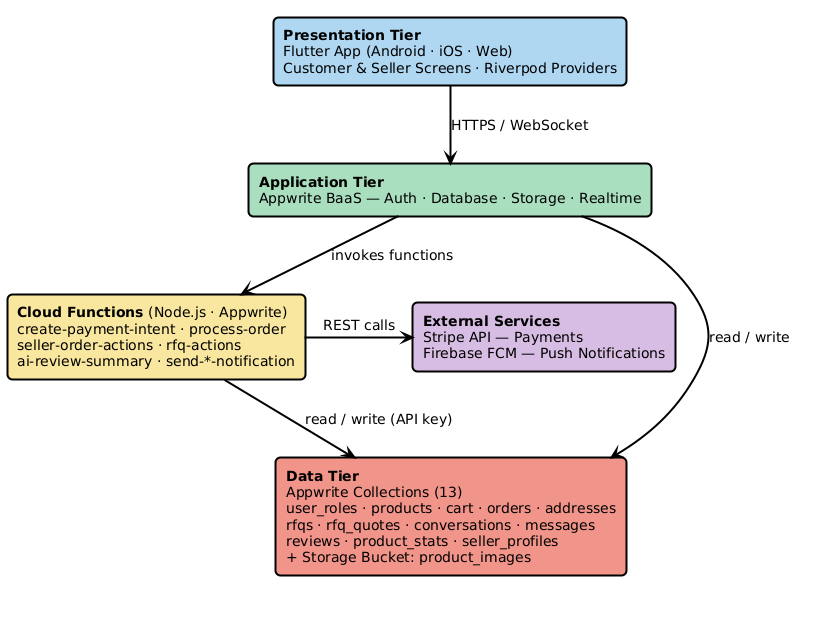
\includegraphics[width=1.1\textwidth]{figures/pictures project/Architecture.png}
\caption{Indus Bazar 3-Tier System Architecture}
\label{fig:system_architecture}
\end{figure}

The architectural illustration in Figure \ref{fig:system architecture} depicts three-tier design of Indus Bazar. Presentation Tier (Flutter app) talks to the Application Tier (Appwrite cloud hosted at fra.cloud.appwrite.io with its serverless functions) via HTTPS. The serverless functions make calls to the Stripe Payments API to create payment intent and Firebase Cloud Messaging API to deliver push notifications. The Data Tier (Appwrite document collections and Storage) can only be accessed via the Appwrite SDK, and all access control policies are implemented on the server-side.

\section{Design Constraints}
This part describes the main constraints and criteria which affect design and development of the Indus Bazar B2B Marketplace.

\subsection{Technical Constraints}
\begin{itemize}
    \item Flutter application is cross-platform (Android, iOS, Web), meaning it has cross-platform requirements on both UI and plugins (e.g. Stripe flutter\_stripe package does not initialise on Web).
    \item Chat Real-time chat needs Appwrite Realtime subscriptions; thus, the message one-to-many collection is designed to allow document events to be streamed in real-time.
    \item All Stripe payments need server-initiated through a cloud function to secure the Stripe secret key; the client simply receives a clientSecret and completes the payment sheet on-locally.
    \item Image uploads: Appwrite Storage using file\_picker with file\_picker and file size and MIME-type validation on the client and at the bucket level.
\end{itemize}

\subsection{Security \& Privacy Constraints}
\begin{itemize}
    \item Email verification This is required: the AppWrapper widget will not allow any navigation to home screens unless isEmailVerified is true; unverified users will always be redirected to the EmailVerificationScreen.
    \item Appwrite Row-Level Security (RLS) document permissions are configured at document creation, and are limited to the owning user(s), restricting read and write access. The seller functions which have to circumvent RLS (e.g., inspecting another users order to update its status) are only carried out within server-side cloud functions with an Appwrite API key.
    \item Stripe publishable key This is the only Stripe credential that is stored in the client-side; the secret key does not exit the create-payment-intent cloud function environment.
    \item Push notification FCM tokens are created in appwrite as a push target child of the authenticated user and unregistered on logout to avoid leakage of notifications.
\end{itemize}

\subsection{Operational Constraints}
\begin{itemize}
    \item The backend is automatically scaled on Appwrite Cloud (Frankfurt region); it does not need an on-premises infrastructure.
    \item cold-starting cloud functions on-demand; latency-sensitive routes (e.g., payment intent) Java lightweight Node.js runtimes to maintain decent response times.
    \item The deduction of product stock at the checkout is managed atomically within the process-order cloud function to avoid overselling when there are concurrent orders.
    \item The RFQ expiry policy (quotes automatically expire on deadline) is implemented with the rfq-actions function to keep the data consistent without client-side timers.
\end{itemize}

\section{Design Methodology}

A mix of Modular Design and Agile Prototyping was used to create Indus Bazar to make it flexible, separate concerns, and deliver working features as the project progressed.

\subsection{Modular Design}

The application itself is broken down into self-contained modules, each containing its own screens, providers, services and models. This separation permits independent development and testing of each domain:

\begin{itemize}
    \item \textbf{Authentication Module} -- Registration, login, email verification, password reset and role assignment (Customer / Seller).
    \item \textbf{Product Catalogue Module} -- Product listing, category filtering and search, product detail, tiered pricing display, multi-image gallery and seller product management (add/edit/deactivate).
    \item \textbf{Cart \& Checkout Module} -- Cart management, quantity sensitive tiered price recalculation, address selection and Stripe payment sheet integration.
    \item \textbf{Order Management Module} -- Customer order history; order status tracking; seller order dashboard with order status progression (pending $\to$ confirmed $\to$ shipped $\to$ delivered).
    \item \textbf{RFQ (Request for Quotation) Module} -- Customer RFQ creation including specifications and target price range; open RFQ marketplace including sellers; sellers submit quote; customer accepts quote and makes payment.
    \item \textbf{Chat \& Messaging Module} -- Per-product chat and messaging between Customer and Seller: Appwrite Realtime! badges to indicate unread messages, and file attaching support.
\end{itemize}

\subsection{Agile Prototyping}
The development was planned as four sprints. At the end of every sprint, there was an incremental functional, testable portion of the application.

\begin{itemize}
    \item \textbf{Sprint 1}: Authentication (registering, logging into, verifying email, role-based routing) and Product Catalogue (browsing, product detail, tiered pricing, seller product management).
    
    \item \textbf{Sprint 2}: Cart Stripe payment integration (cloud functionality + payment sheet), Customer and Seller Order Management and Address management.
    
    \item \textbf{Sprint 3}: RFQ system (creation, open marketplace, quote submission and acceptance, RFQ-based payment) and real-time Chat \& Messaging with Appwrite Realtime.
    
    \item \textbf{Sprint 4}: Review system, verified-purchase enforcement, AI-generated review summaries, Seller Profile management, and FCM push notification delivery of all key events.
\end{itemize}

Each sprint involved planning, development, testing, and feedback to have interdependency among modules sorted out early and the final system was able to satisfy all functional requirements.

\section{System Activity Diagram}

The general workflow of Indus Bazar is described through activity diagrams, which illustrate the end-to-end processes of its two main user roles, Customer and Seller, starting with the process of logging in until the final stages of completing the commercial transactions. These charts are graphical representations of the flow of activity, decision-making and system feedback to perform different functionalities of the platform. The activity diagrams demonstrate the way users make contact with the system and data movement between the modules are well established thus creating clear understanding of the processes of operation. They emphasize the rational flow of actions, activities simultaneity, and conditional branching that takes place in the real-time operations in the B2B marketplace.

\subsection{Customer Activity Diagram}

To the Customer, the activity diagram illustrates user authentication, product discovery, viewing product details, RFQs, communicating with sellers over real-time chat, adding items to the shopping cart, checkout, and secure payments with Stripe, and order status tracking. It also incorporates the optional directions towards negotiating quotes, reviewing products, and reading AI-generated review summaries. The workflow starts with customer registration/ log-in, then email verification where the customers are assured safe access to the platform. When authenticated, customers are able to view categorized listings of products, filter using advanced search filters and compare tiered pricing structures before they make purchase decisions. 

Figure \ref{fig:customer_activity_diagram} represents the overall end-to-end process of a registered customer in Indus Bazar B2B marketplace. This is done by registering a new user by entering his full name, email address, password, and Customer role. When registration is successful, an automatic verification email will be sent through Appwrite. The customer has to authenticate their email prior to access and the AppWrapper widget constantly checks the authentication status and blocks unverified users. Upon verification, the customer is redirected to Customer Home screen, the main center of all activities in the platform. There are two major procurement paths enabled in the Customer Home screen that are: \textbf{Direct Purchase} and \textbf{RFQ (Request for Quotation)}. Under the Direct Purchase route, a customer navigates through the product catalogue with search and filter options, looks through the product specifications, including tiered pricing, places an order by the required quantity, and adds to the cart. 

\begin{figure}[htbp]
\centering
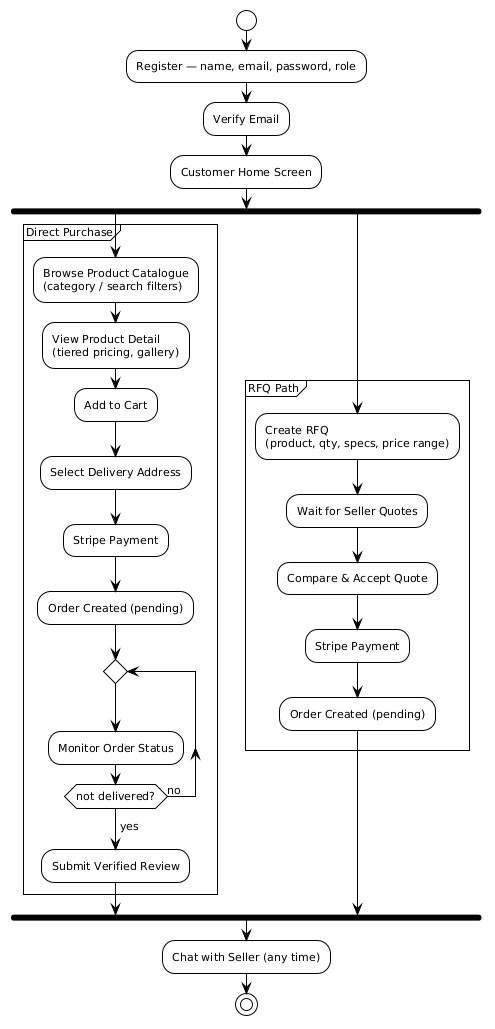
\includegraphics[width=0.72\textwidth]{figures/pictures project/Customer_Activity_Diagram.png}
\caption{Customer Activity Diagram}
\label{fig:customer_activity_diagram}
\end{figure}

The customer activity diagram in Figure \ref{fig:customer_activity_diagram} will help demonstrate the entire end to end process of a registered customer in the Indus Bazar B2B marketplace. This is done by registering a new user by entering his full name, email address, password, and Customer role. When registration is successful, an automatic verification email will be sent through Appwrite. The customer has to authenticate their email prior to access and the AppWrapper widget constantly checks the authentication status and blocks unverified users. Upon verification, the customer is redirected to Customer Home screen, the main center of all activities in the platform.

There are two major procurement paths enabled in the Customer Home screen that are: \textbf{Direct Purchase} and \textbf{RFQ (Request for Quotation)}. Under the Direct Purchase route, a customer navigates through the product catalogue with search and filter options, looks through the product specifications, including tiered pricing, places an order by the required quantity, and adds to the cart. At checkout, the customer verifies the shipping address and finalizes the payment safely with Stripe using credentials that are generated by the server. The system will automatically make the order, update inventory and send confirmation and push notifications on successful payment. The Orders screen allows customers to monitor the status of their orders in real time.

Bulk procurement or customized procurement is supported on the RFQ path. Customers place an RFQ with product requirements and quantities, location of delivery, specifications, and optional price ranges. The RFQ is posted to the market, and the sellers are allowed to make competitive bids. Customers read and compare the quotes received, pick the most appropriate offer and continue on the reliable Stripe payment flow. Once payment is confirmed, the system will create an order based on the accepted quotation and will shut-down the RFQ to additional bids to provide a smooth and transparent procurement process.


\subsection{Seller Activity Diagram}
To the Seller, the diagram describes the following activities: registration and verification of accounts, product listing and catalog, managing tiered pricing, RFQ responses, customer interaction in the chat system, receiving orders, updating order status, and delivery. It also emphasises administrative activities like tracking sales performance, handling quotations, and customer feedback. These charts also illustrate system-level processes of email verification, push notifications, secure payment processing, and automated order creation. Conditional flows, including the success or failure of a payment, the acceptance or rejection of an RFQ, and the confirmation or cancellation of an order are drawn using decision nodes.

Moreover, the activity diagrams have integrations with third-party services, such as Stripe to process secure payments, Appwrite to implement backend services and cloud functions, and Firebase Cloud Messaging (FCM) to implement real-time push notifications. These integrations guarantee a responsive, scalable and secure platform. The System Activity Diagrams can be used as a powerful reference resource by developers, stakeholders, and system analysts by offering the visual representation of user interactions and backend processes in a comprehensive manner. They enable system insight, authenticate functional requirements, and enable effective implementation, testing, and addition of the Indus Bazar B2B Marketplace in the future.
\begin{figure}[htbp]
\centering
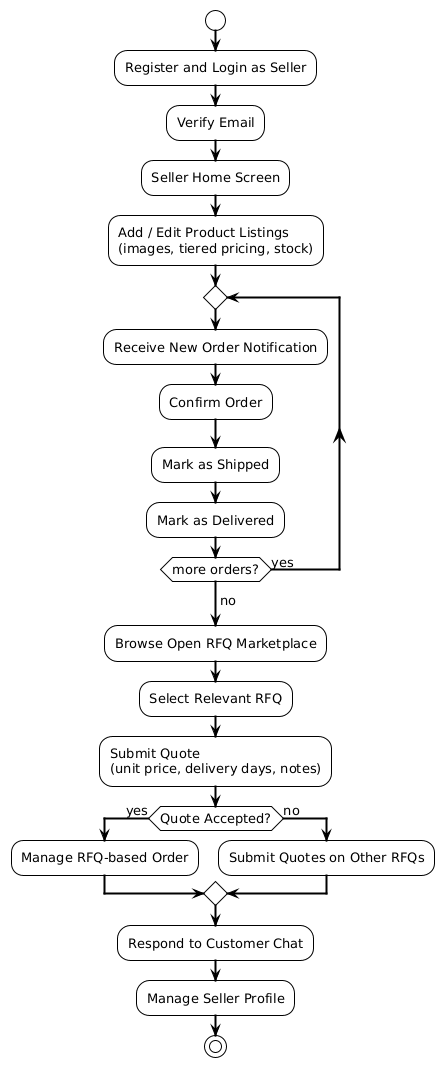
\includegraphics[width=0.61\textwidth]{figures/pictures project/Seller_Activity.png}
\caption{Seller Activity Diagram}
\label{fig:seller_activity_diagram}
\end{figure}

The seller activity diagram (Figure \ref{fig:seller_activity_diagram} presents the entire workflow a registered seller has in the Indus Bazar platform. The process starts with the registration and email verification, then the seller is redirected to the Seller Home, which is a main dashboard of all operations related to the sellers. Out of this hub there are two parallel streams of operation that the seller can be involved in either at the same time or alternately as per the business need.

At the stream Product and order management, the seller starts by developing and maintaining his or her product catalogue. The products listing contains a name, description, category, stock quantity, up to three images of the product uploaded to the Appwrite Storage, and a price structure based on tiers which enables the seller to provide lower unit prices with increased order volume a core aspect of B2B procurement. As soon as listings are active, the seller sees the customer orders that are coming in via the Seller Orders screen. Every new order will send out a push notification to the device of the seller, and no order will go undetected. The seller then completes each order by following the established lifecycle phases where receipt is established, the order is marked as shipped after dispatched and finally it is marked as delivered after successful handover that keeps the customer updated at every stage through automatic status updates.

Through the \textbf{RFQ Response} stream, the seller visits the open RFQ marketplace, which consolidates all the active Requests for Quotation placed by customers in the platform. The seller identifies RFQs associated with their product catalogue, examines specifications and target price range of the customer and sends a competitive quote, which includes unit price, total price, estimated delivery days and any other notes. When the customer accepts a quote made by the seller then an order is automatically generated and is handled by the same order lifecycle as direct purchases. The seller can also reply to customer messages at any stage of both streams using the integrated real time chat system and retain first person contact to be able to clarify product details or bargain. The seller is also able to access and update his or her public seller profile that will show his or her business name, city, contact details and aggregate rating aspects which directly affect buyer confidence and their buying choices.

\section{High Level Design}
High Level Design (HLD) displays the key building blocks of the Indus Bazar, interactions between them, and topology. The HLD does not include the specifics of implementation, but gives a bird-eye view of how the components of the system work together to provide B2B marketplace functionality.

\subsection{Component Diagram}
The Component Diagram will define the key software elements of Indus Bazar and interfaces with each other.

\begin{figure}[H]
\centering
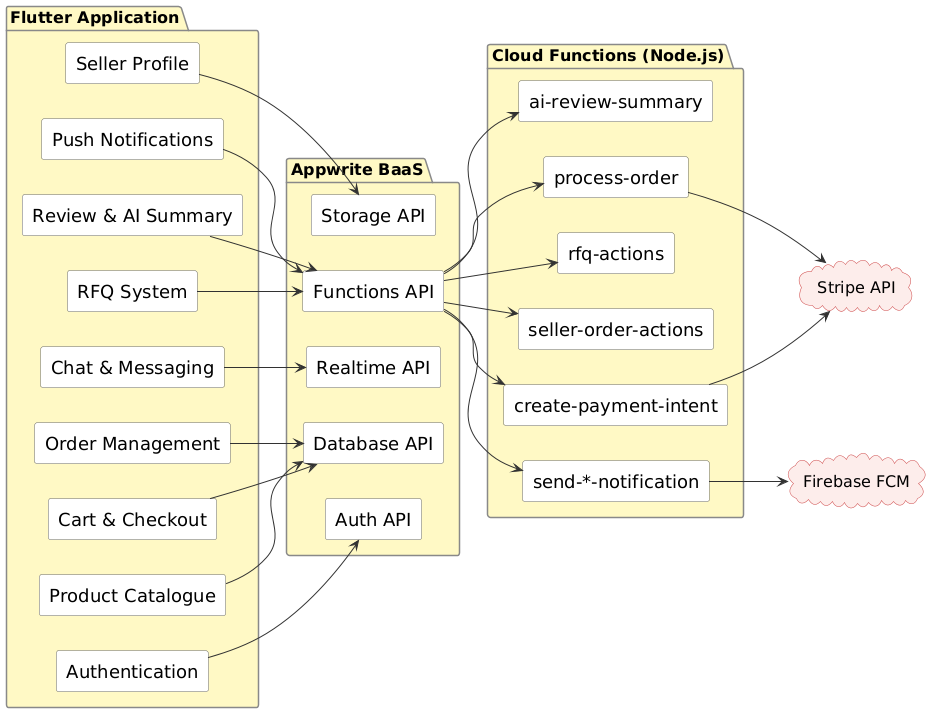
\includegraphics[width=1.0\textwidth]{figures/pictures project/component_diagram.png}
\caption{Component Diagram}
\label{fig:component_diagram}
\end{figure}

The component diagram in Figure \ref{fig:component_diagram} depicts the modular configuration of Indus Bazar. The Presentation Tier is comprised of the Flutter application that includes 9 logical sub-elements: Authentication, Product Catalogue, Cart / Checkout, Order Management, RFQ System, Chat / Messaging, Review / AI Summary, Seller Profile, and Push Notification processing. These sub-components communicate with the layer of the Appwrite BaaS through the official Dart SDK (appwrite: \^{17.1.0}), which opens the Appwrite Account, Database, and Storage APIs, Functions, and Realtime APIs. The Appwrite interface to two third-party services is provided by the \textbf{Appwrite Cloud Functions} component (eight Node.js serverless functions) which connects Appwrite to the Stripe Payments API (to create a payment-intent) and the Firebase Cloud Messaging API (to send a push-notification). The core Appwrite Database (document collections) and Appwrite Storage (product and review images) are shared data sources which can be accessed by the client SDK and the cloud functions.


\subsection{Deployment Diagram}

The Deployment Diagram shows the physical and logical nodes on which the Indus Bazar system components are hosted and how they communicate in a production environment.

\begin{figure}[H]
\centering
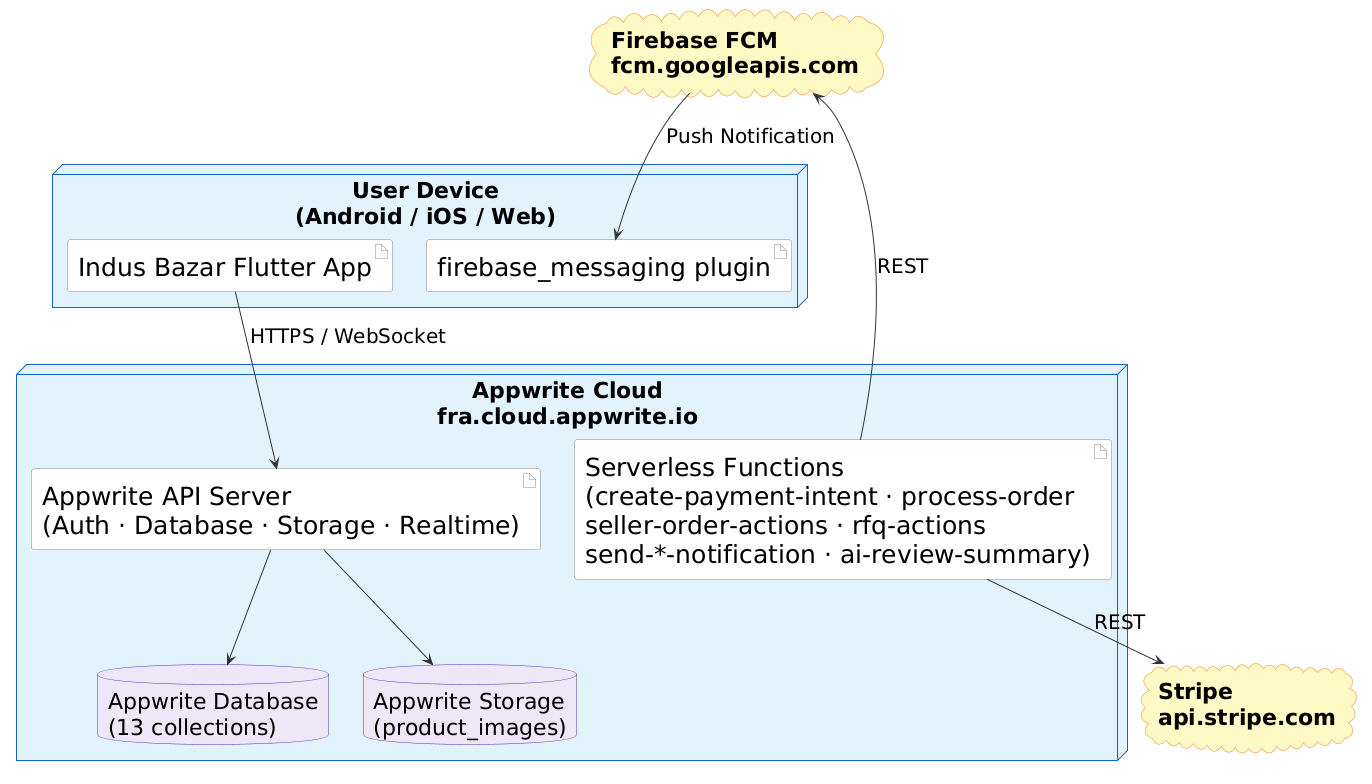
\includegraphics[width=1.0\textwidth]{figures/pictures project/deployment_diagram.png}
\caption{Deployment Diagram}
\label{fig:deployment_diagram}
\end{figure}

The deployment topology of Indus Bazar is depicted in the deployment diagram, as represented by Figure \ref{fig:deployment_diagram}. Flutter is executed as a native binary on the User's Device (Android or iOS) or a Progressive Web App in the browser. All backend requests are deployed to the Appwrite Cloud (located in the Frankfurt region at fra.cloud.appwrite.io) which contains internally the Appwrite API server, document database, file storage bucket, the Realtime subscription broker, and the serverless function runtime. The cloud functions call the Rest API of Stripe (api.stripe.com) to process payments and push notification delivery using Firebase Cloud Messaging (fcm.googleapis.com). The firebase\_messaging Flutter plug handles device-side notification handling by receiving the message sent by FCM.

\section{Sequence Diagrams}

The sequence diagrams in this section trace the interaction of the Flutter application, Appwrite services and external APIs to achieve each major feature of Indus Bazar. The diagrams show the appropriate actors, subsystems and system components, and provide a clear way of seeing the exact sequence of messages sent back and forth, the flow of data and the control logic used in the implementation of core functionalities within the platform. These charts emphasize both the synchronous and asynchronous communications, backend operations via Appwrite cloud functions, and secure connections with third-party services like Stripe to handle payments and Firebase Cloud Messaging to receive push notifications. The sequence diagrams offer an informative temporal perspective of how the system interacts with other systems, which verify the functional requirements and are useful in developing the system efficiently, debugging, testing, and scaling the Indus Bazar B2B marketplace in the future.

\clearpage
\subsection{Registration \& Login Sequence}

{\centering
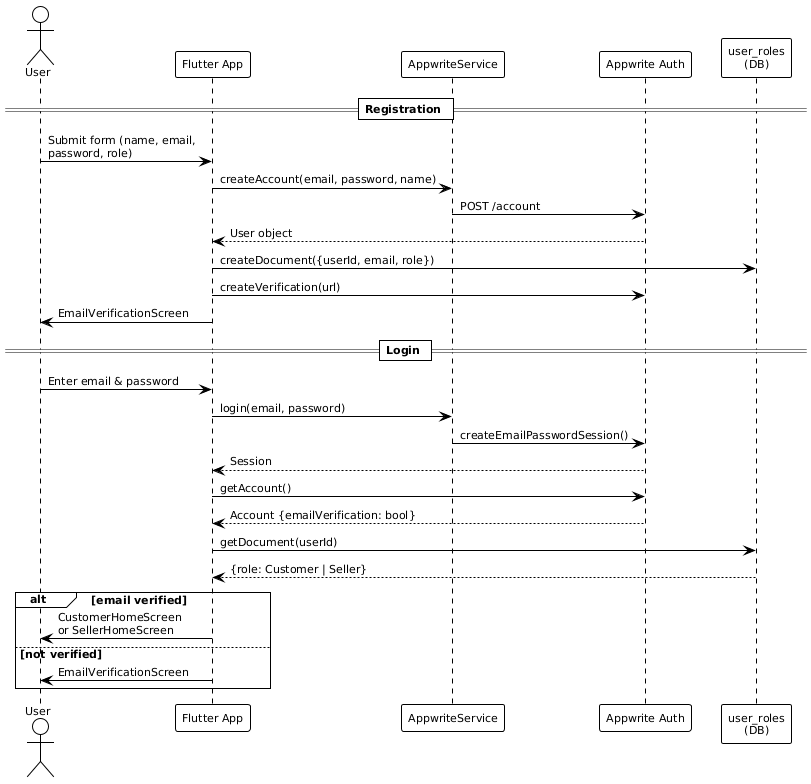
\includegraphics[width=\textwidth,height=0.75\textheight,keepaspectratio]{figures/pictures project/SEQUENCE1.png}\par
\captionof{figure}{Registration and Login Sequence Diagram}
\label{fig:login_sequence}\par}
\vspace{2em}

The sequence diagram of registration and login process \ref{fig:login_sequence} shows the two step onboarding process. In the course of the registration, the Flutter application invokes AppwriteService.createAccount, a call to the Appwrite Account API to create a new user. The selected role (Customer or Seller) is written to the collection of user roles in a follow up call, and an email verification message is sent. The user is then taken to the EmailVerificationScreen. At login, the app invokes AppwriteService.login(appwrite) that establishes an email-password session. Only when the validation is found, the AuthProvider gets the current account and role, verifies emailVerification status and redirects to the correct home screen (CustomerHomeScreen or SellerHomeScreen). Conflicts that occur during existing-session are managed in a transparent manner by catching the user\_session\_already\_exists error and reusing the valid session.

\subsection{Product Browsing \& Direct Purchase Sequence}

{\centering
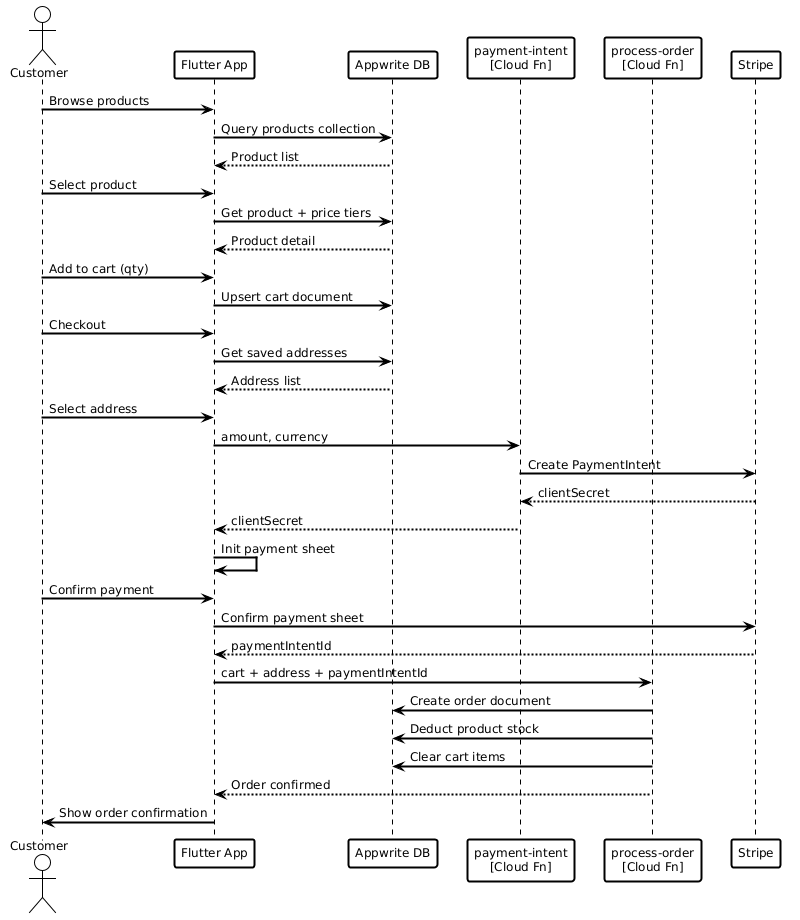
\includegraphics[width=\textwidth,height=0.75\textheight,keepaspectratio]{figures/pictures project/SEQUENCE2.png}\par
\captionof{figure}{Product Browsing and Direct Purchase Sequence Diagram}
\label{fig:product_browse_sequence}\par}
\vspace{2em}

The direct purchase sequence product browsing and direct purchase sequence \ref{fig:product_browse_sequence} encompasses the process of catalogue discovery to final payment. The customer clicks on ProductBrowseScreen, which calls upon ProductProvider to query the Appwrite products collection with optional category and search filters. When a product is selected, the ProductDetailScreen retrieves all the product information such as all price points and the seller profile and shows the tiered price structure. The customer enters the required amount to the cart; the CartProvider calculates the appropriate tier price and inserts a document into the cart collection. The customer chooses one of the saved addresses (or adds one to the addresses collection) at checkout, and PaymentProvider makes a create-payment-intent cloud call to StripeService, which returns a clientSecret. The Flutter Stripe payment sheet is loaded and shown; when it is confirmed Stripe returns a paymentIntentID, forwarded to the process-order cloud function. That atomically inserts the order document into the orders collection, removes stock off the product document and clears the cart items all under API-key authority of the server to pass through RLS.

\subsection{RFQ Creation \& Quote Acceptance Sequence}

{\centering
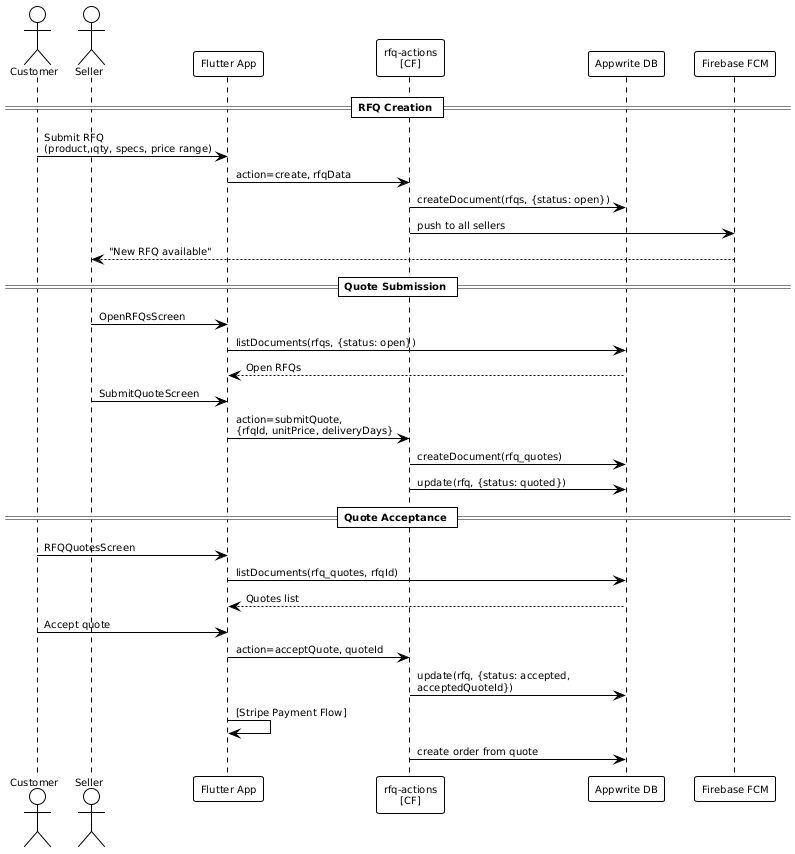
\includegraphics[width=\textwidth,height=0.75\textheight,keepaspectratio]{figures/pictures project/SEQUENCE3.png}\par
\captionof{figure}{RFQ Creation and Quote Acceptance Sequence Diagram}
\label{fig:rfq_sequence}\par}

The RFQ sequence diagram \ref{fig:rfq_sequence} follows the entire lifecycle of a Request for Quotation. The customer browses to CreateRFQScreen and sends a request with the name of products, category, quantity, city of delivery, deadline, specifications and optional target price range. The rfq-actions cloud function creates an RFQ document in the rfqs collection with status open and broadcasts a push notification via the send-rfq-notification function to all sellers. When an RFQ is made open, the sellers see it on OpenRFQsScreen, choose one of the relevant requests, and send the quote using SubmitQuoteScreen--the functionality stores the quote in rfq\_quotes and changes the status of the RFQ to quoted. RFQQuotesScreen: The customer evaluates all the quotes received and accepts one of them and goes to the payment flow through the same Stripe payment-sheet as with direct purchase. When payment is confirmed the process-order function produces the appropriate order and the RFQ status changes to accepted.

\subsection{Order Processing Sequence}

{\centering
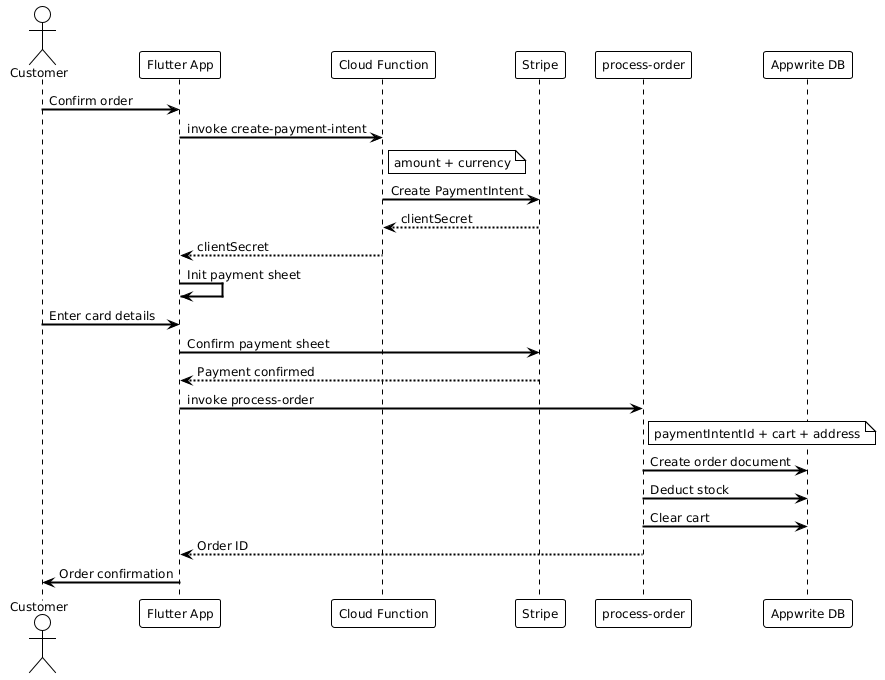
\includegraphics[width=\textwidth,height=0.75\textheight,keepaspectratio]{figures/pictures project/SEQUENCE4.png}\par
\captionof{figure}{Order Processing Sequence Diagram}
\label{fig:order_sequence}\par}

\vspace{1em}
The order processing sequence \ref{fig:order_sequence} shows the flow of order through its lifecycle after it has been created. When order document is present in the orders collection with the status pending, send-order-notification function sends an FCM push notification to the seller. The new order is displayed to the seller on the SellerOrdersScreen and can be viewed by the seller on SellerOrderDetailScreen (its contents, delivery address, contact with the customer) The seller actions (confirm, ship, deliver, cancel) are directed to the seller-order-actions cloud function that updates the order document status under API-key authority (bypassing the customer-only RLS on that document) and sends the corresponding send-order-notification call to ensure that the customer gets a live push notification. Status is followed by customer using the OrdersScreen.

\subsection{Real-Time Chat Sequence}

{\centering
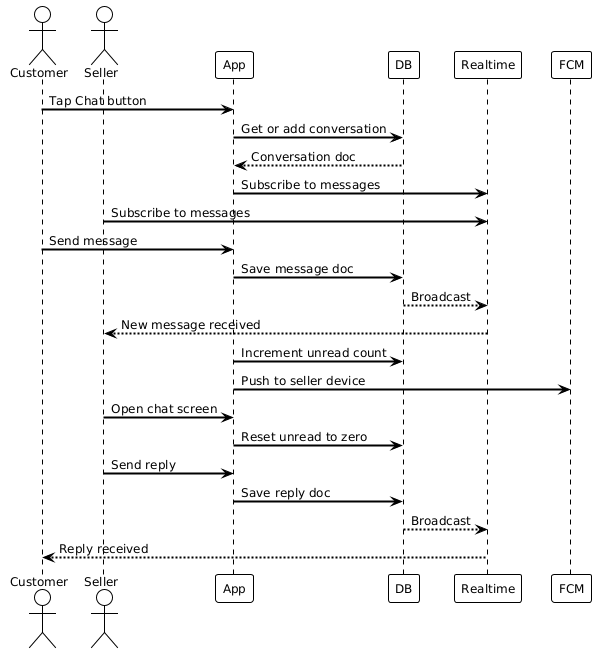
\includegraphics[width=\textwidth,height=0.75\textheight,keepaspectratio]{figures/pictures project/SEQUENCE5.png}\par
\captionof{figure}{Real-Time Chat Sequence Diagram}
\label{fig:chat_sequence}\par}

\vspace{1em}
The real-time chat sequence \ref{fig:chat_sequence} covers the establishment and operation of a product-scoped conversation between a customer and a seller. Upon the customer tapping the chat button on ProductDetailScreen, ChatService.getOrCreateConversation() searches the conversations collection to find an existent thread with key (customerId, sellerId, productId). In case none is available, a new conversation document is created with per-user Read and Update permissions. The ChatScreen is opened by both parties and subscribes to the Appwrite Realtime channel used to collect the messages with a conversationId filter. Messages sent are written to the messages collection and are immediately sent to all subscribers. When the send-chat-notification function is called every time to send a FCM notification to the recipient.

\subsection{Push Notification Delivery Sequence}

{\centering
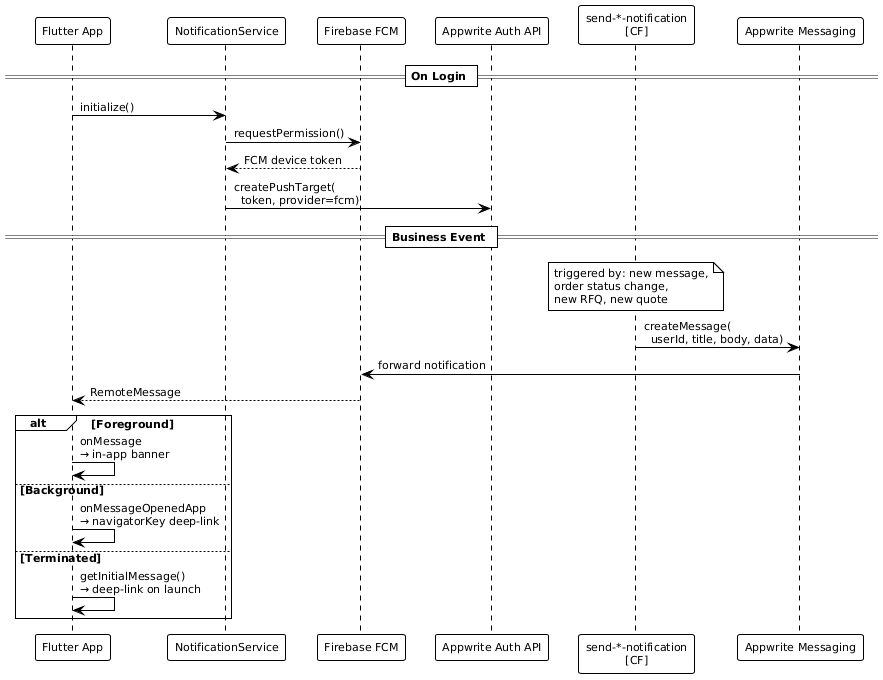
\includegraphics[width=\textwidth,height=0.75\textheight,keepaspectratio]{figures/pictures project/SEQUENCE6.png}\par
\captionof{figure}{Push Notification Delivery Sequence Diagram}
\label{fig:notification_sequence}\par}

\vspace{1em}
The notification delivery sequence \ref{fig:notification_sequence} shows the end to end flow of the event that triggers the notification, as well as the flow to the device of the recipient. Upon login, the Notificationservice makes a request to FCM permission, obtains the device FCM token and registers it as an Appwrite push target with the scope of the authenticated user. Upon a business event happening (new chat message, order status change, new RFQ, new quote), the call of the Appwrite Messaging API with the API key is made to generate a push message that will be sent to the relevant user registered FCM token. The message is sent to the Firebase Cloud messaging service, which sends it to the target device, through Appwrite. FirebaseMessaging is the notification that is processed by the firebase\_messaging plugin: when the app is in the foreground, it is FirebaseMessaging.onMessage is fired; when the app is in the background or terminated, onBackgroundMessage or getInitialMessage is called. On notification tap, the navigatorKey is used by \_handleNotificationTap (e.g., chat, order detail, RFQ list) to deep-link the user to the appropriate screen.

\section{Low Level Design}

Low Level Design (LLD) outlines data structures and entity relationships on which the Indus Bazar system will be based. All long-term data is stored in the NoSQL document collections in Appwrite; the schema below defines the values and relationships of each collection.

\subsection{UML Class Diagrams}
The Indus Bazar data model includes thirteen collections. The UML Class diagrams below illustrate the attributes of the entities and the referential associations to be kept using stored ID fields, which is a document-oriented database as Appwrite is.

\begin{figure}[H]
\centering
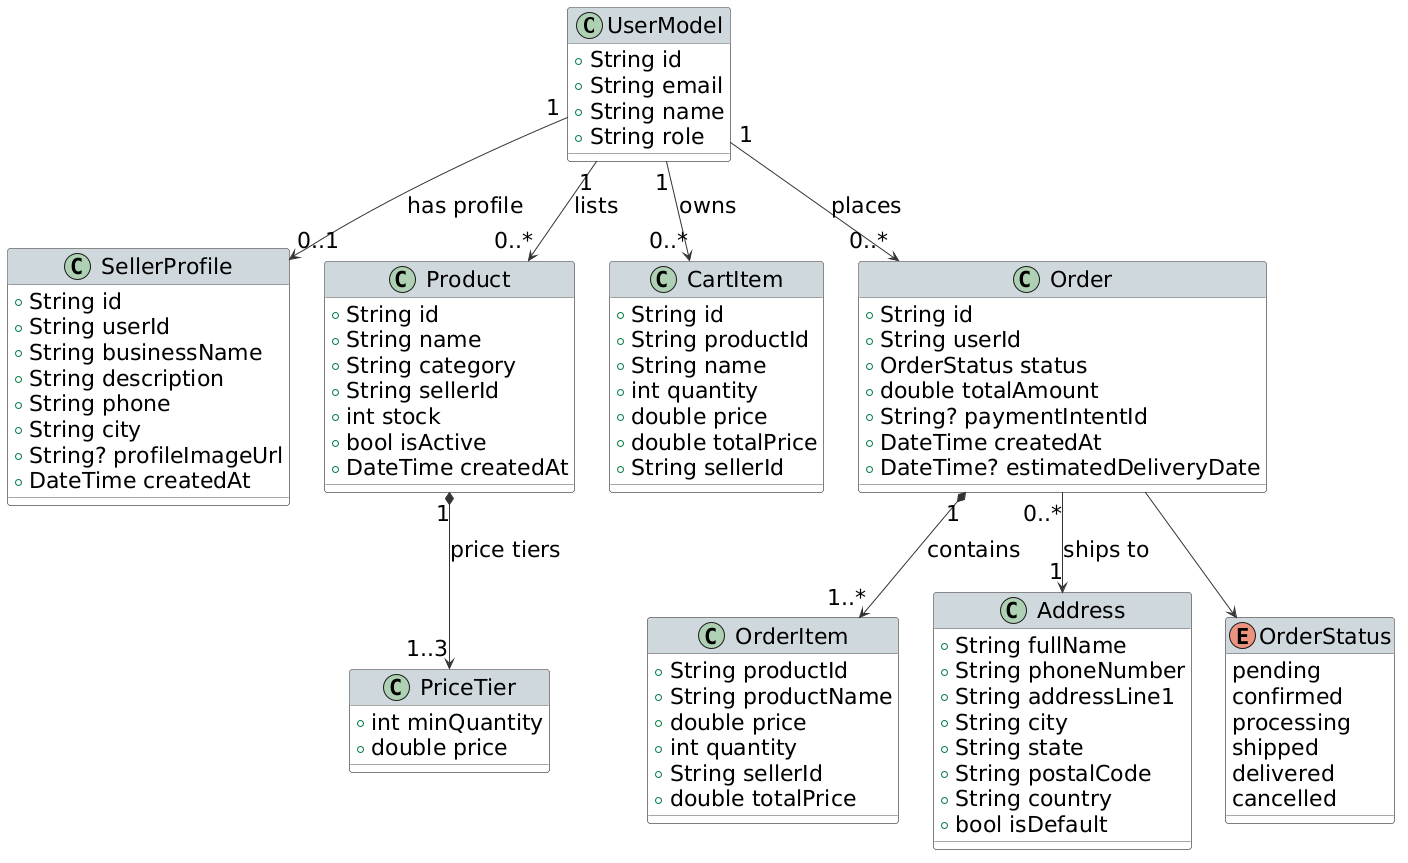
\includegraphics[width=0.95\textwidth]{figures/pictures project/UML_CLASS1.png}
\caption{Core Entity Relationship Diagram --- User, Product, Cart, Order, and Address Entities}
\label{fig:main_erd_schema}
\end{figure}

The backbone UML in Figure \ref{fig:main_erd_schema} deals with the transactional core of the marketplace. The \textbf{UserRoles} entity contains the following: userId, email, role (Customer / Seller), and fcmToken. The Product entity has name, description, category, sellerId, sellerName, stock, isActive, and up to three tiered price bands (tier1MinQty/tier1Price to tier3MinQty/tier3Price), with the imageUrls as a JSON-encoded array. The \textbf{CartItem} entity connects a user id to product id with a specified quantity. The \textbf{Order} object is a collection of customer information, a JSON array of items (each item is a productID, productName, price, amount, sellerID) total amount, status, paymentintentid and an embedded address. \textbf{The Address} entity holds street, city, province, postalCode and country and is referenced by both the order documents and the separate addresses collection of individual users.

\begin{figure}[H]
\centering
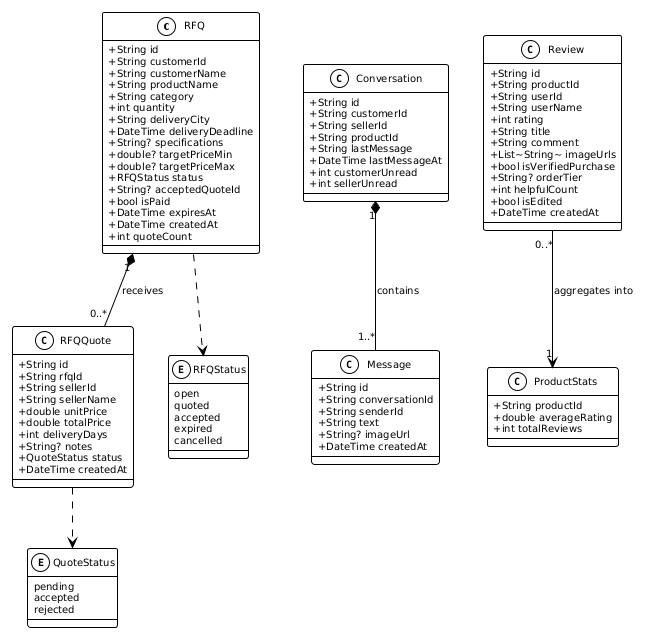
\includegraphics[width=0.95\textwidth]{figures/pictures project/UML_CLASS2.png}
\caption{Extended Entity Relationship Diagram --- RFQ, Chat, Review, and Seller Profile Entities}
\label{fig:extended_erd_schema}
\end{figure}

Figure \ref{fig:extended_erd_schema} is an extended UML that addresses the marketplace-specific and communication entities. The \textbf{customerId}, \textbf{category}, \textbf{productName}, \textbf{quantity} and \textbf{deliveryCity}, \textbf{deliveryDeadline}, \textbf{specifications}, optional \textbf{targetPriceMin/targetPriceMax}, \textbf{status (open / quoted / accepted / expired / cancelled)} and \textbf{expiresAt} are captured in the entity called the RFQ. Every \textbf{rfqQuote} is associated with a \textbf{sellerId} and \textbf{rfqId} having \textbf{unitPrice}, \textbf{totalPrice}, \textbf{leadTimeDays}, \textbf{notes} and a \textbf{status (pending / accepted / rejected)}. The \textbf{Conversation} entity has three-way key \textbf{customerId}, \textbf{sellerId}, and \textbf{productId}, \textbf{lastMessage}, \textbf{lastMessageAt}, \textbf{customerUnread}, and \textbf{sellerUnread}. Every \textbf{Message} is a member of a \textbf{conversationId} and contains \textbf{senderId}, \textbf{text}, \textbf{imageUrl} and \textbf{createdAt}. The \textbf{Review} entity associates a \textbf{userId} with a \textbf{productId} and storing \textbf{rating (1-5)}, \textbf{title}, \textbf{comment}, \textbf{JSON-encoded imageUrls}, \textbf{isVerifiedPurchase}, \textbf{helpfulCount} and \textbf{helpfulByUsers}. \textbf{ProductStats} is a pre-aggregated \textbf{averageRating}, \textbf{totalReviews}, and \textbf{rating-distribution counts}, per product. The \textbf{SellerProfile} table contains the attributes \textbf{userId}, \textbf{businessName}, \textbf{description}, \textbf{phone}, \textbf{address}, \textbf{city} (and \textbf{cityLower} as case-insensitive geosearch) and \textbf{profileImageUrl}.


\section{GUI Design}

The Indus Bazar mobile interface is structured on the concept of a role-adaptive experience: the application will have a different home screen and a flow of navigation depending on the role of the authenticated user (Customer or Seller). It is designed according to the Material Design 3 standards, with a custom AppTheme and looks into the usage of Google fonts, shimmer loading placeholders, cached\_network image as an efficient way to display images, and lottie animation as an empty and loading state. Every screen is created as HookConsumerWidgets, which rebuilds on Riverpod provider state changes.

\vspace{2em}

\begin{figure}[H]
\centering
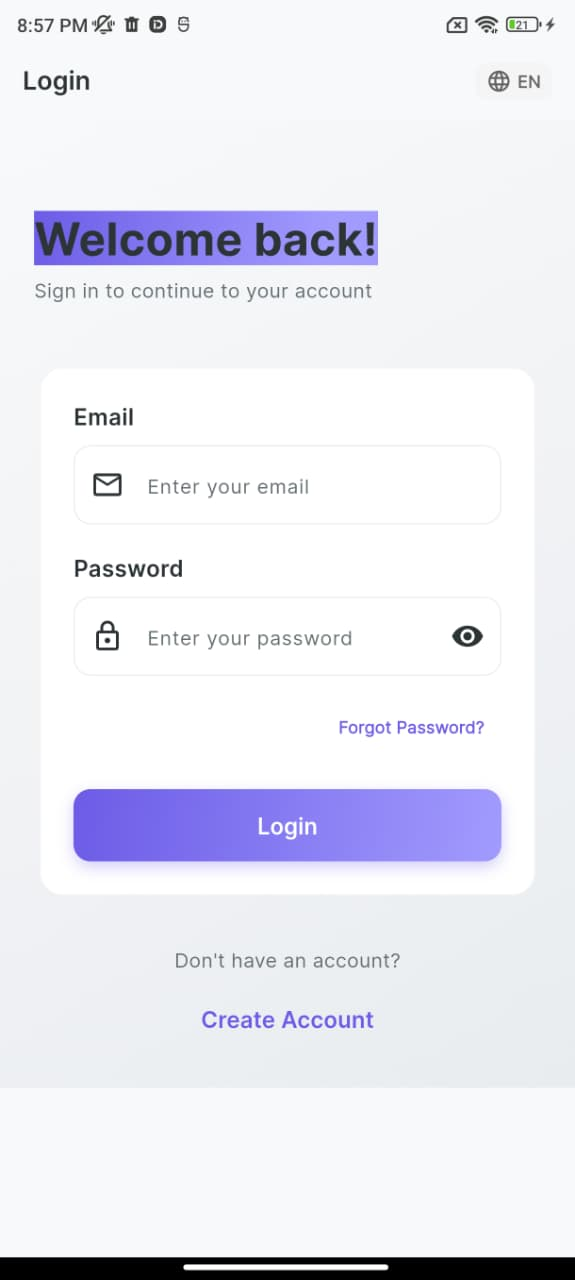
\includegraphics[width=0.4\textwidth]{figures/pictures project/frontend/login.jpeg}
\caption{Login Screen Interface}
\label{fig:login_screen}
\end{figure}

Figure \ref{fig:login_screen} shows the login interface of Indus Bazar. The screen offers a clear and bare bone of the registered user, and the input fields of email and password are assigned, a toggle of visibility of password is available, an option to forget password is present, and a large login button is presented on the screen. There is also a language switch in the upper right-hand corner where the user may switch language of the interface to proceed with the authentication. In terms of usability, the screen minimizes cognitive load by displaying minimal actions when signing in. The visual hierarchy established through the headline, form card and primary action button assist the user to learn the purpose of the page in a few seconds. The large distance between the input fields is also a good way to enhance the readability and touch response of the mobile devices. The design creates a very appropriate first-time and returning user experience since it does not have any distractions that would give the impression of a repetitive authentication pattern. Moreover, the form layout promotes validation and error messages in such a manner that they can be incorporated without disrupting the overall balance of the screen. Consequently, the login screen serves as a secure authentication point as well as the properly designed starting point of the role-based navigation of the application.


\begin{figure}[H]
\centering
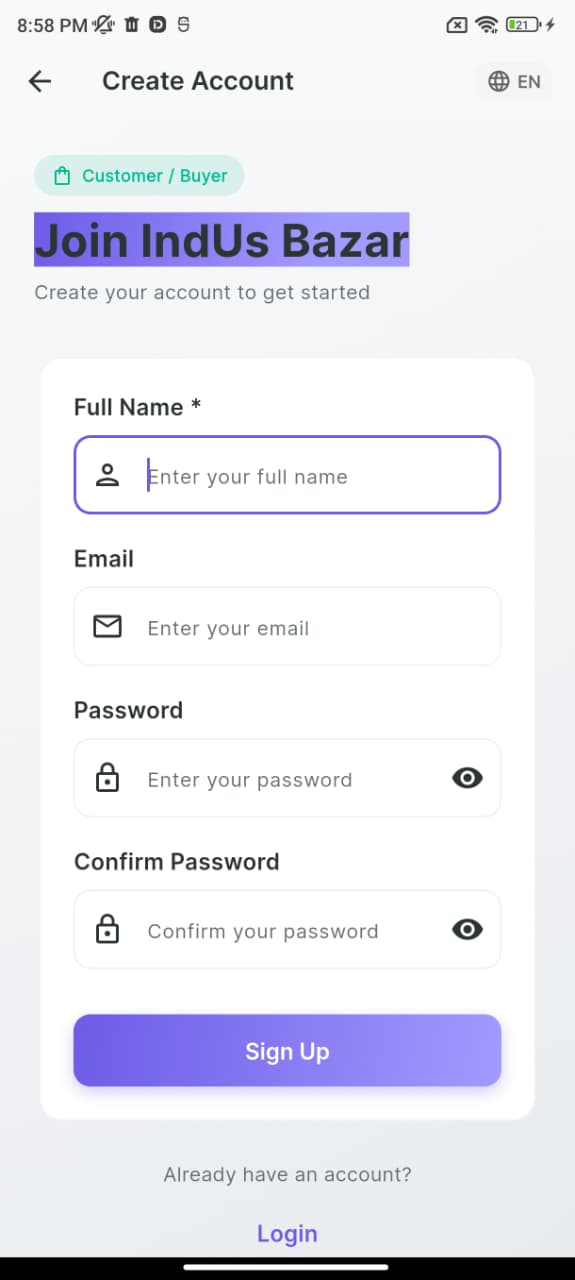
\includegraphics[width=0.4\textwidth]{figures/pictures project/frontend/signup.jpeg}
\caption{Registration Screen Interface}
\label{fig:signup_screen}
\end{figure}

Figure \ref{fig:signup_screen} presents the customer registration screen. The interface takes the required onboarding information such as full name, email address, password, password confirmation, and it has made it clear which role has been selected as Customer / Buyer. Its simple design enables less friction when creating an account and directs new users to the platform with the least friction. The shape will ensure that the onboarding process is explicit and linear so that users do not have to go through several steps before they complete the registration process. The role indicator is particularly essential in a two-role marketplace as it avoids confusion in creating customer and seller accounts. The visual consistency to the login screen also makes the users feel that the two screens are part of the same secure authentication process. The form is simple, with only one main sign-up button, which promotes form completion and maintains the model of interaction. This screen thus becomes significant in converting unidentified users into authenticated ones who can enjoy more of the market place. It also provides the first identity context that subsequently manages the role-based dashboard routing and permission-handling.

\begin{figure}[H]
\centering
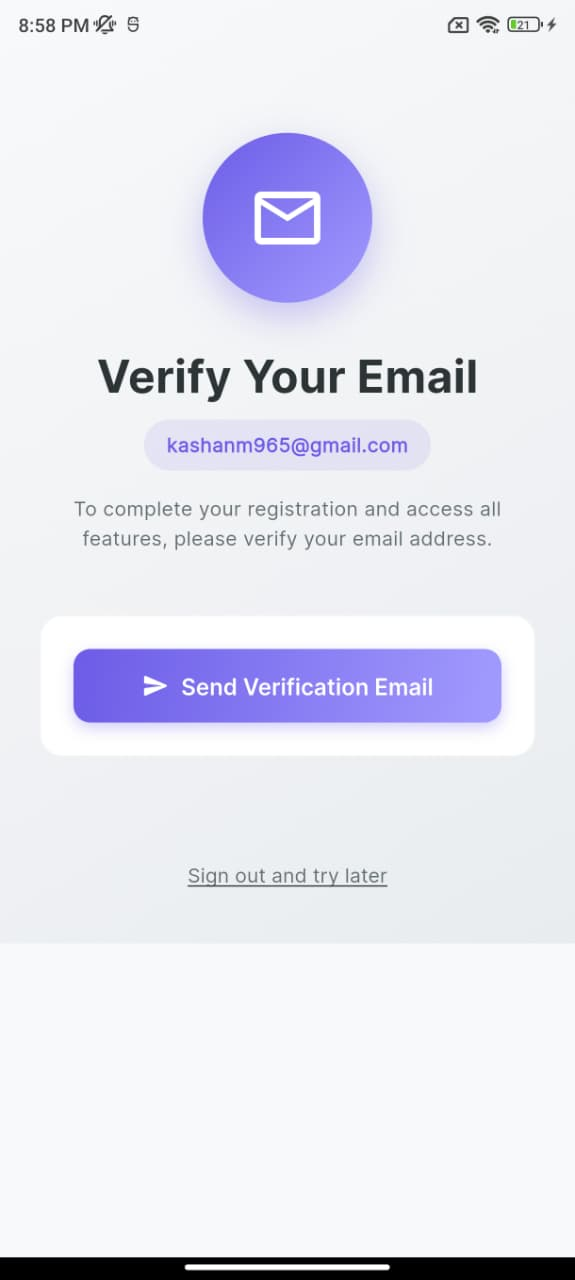
\includegraphics[width=0.4\textwidth]{figures/pictures project/frontend/email verification.jpeg}
\caption{Email Verification Screen Interface}
\label{fig:email_verification_screen}
\end{figure}

\clearpage

Figure \ref{fig:email_verification_screen} shows the email verification screen which appears after the registration. The screen notifies the user that they must activate the account to use the marketplace features and offers a specific action to resend the verification email in case it is necessary. This interface assists with the security need of the system that only a verified account can be given access to the main application. The use of the middle-ground composition and the targeted message makes it more than clear what the screen is all about and makes the user less likely to be confused post-account creation. The interface also informs the user that the request to verify his/her email address has been sent by showing him/her the email address and also reminds him/her in case of typing errors. Reliability is also significant with resend action, when mail delivery can be delayed, or lost messages. The signature out and resume option also conforms to the real world user behaviour, by permitting temporary suspension without disrupting the flow. Security wise, this screen enhances the degree of trust because it physically implements account validation as opposed to unverified access. Generally, it serves as a gate between registration and the actual system use.

\begin{figure}[H]
\centering
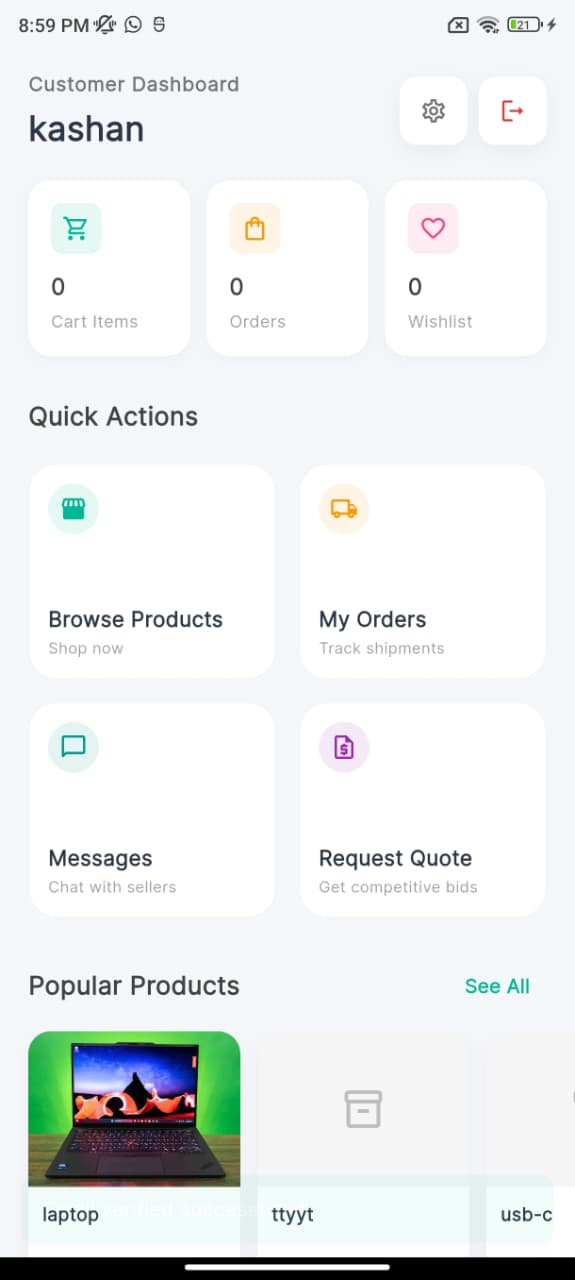
\includegraphics[width=0.4\textwidth]{figures/pictures project/frontend/customer dashboard.jpeg}
\caption{Customer Home Screen Interface}
\label{fig:customer_home}
\end{figure}

\clearpage
The customer home dashboard as depicted in Figure \ref{fig:customer_home} serves as the main area of navigation when the customer is already logged in. It provides an overview of important user metrics (cart items, orders, and wishlist items), and has quick-action cards to browse the products, track the orders, open the messages and create RFQs. There is also a popular products section to bring out featured items and stimulate product discovery. This screen has been created to reduce the effort of navigation because the most common customer activities are put together. The metric cards also give the client a real-time feedback on what is going on in the marketplace and make the user know their position within the application. Quick-action tiles are visual shortcuts that minimise the amount of steps that have to be followed in between to get to the popular workflows. The featured or popular products are also added to the dashboard turning the dashboard into a commercial discovery-based surface rather than the functional one. This plays a critical role in a B2B market where decisions to buy are frequently influenced by repeated shopping and comparison of products. The dashboard thus contributes not only to efficiency in carrying out the tasks, but also to engagement with the product, thus, being a vital aspect of the customer experience. The role-adaptive design philosophy can be seen in its design as well since it reveals functions that are pertinent to buyers.

\begin{figure}[H]
\centering
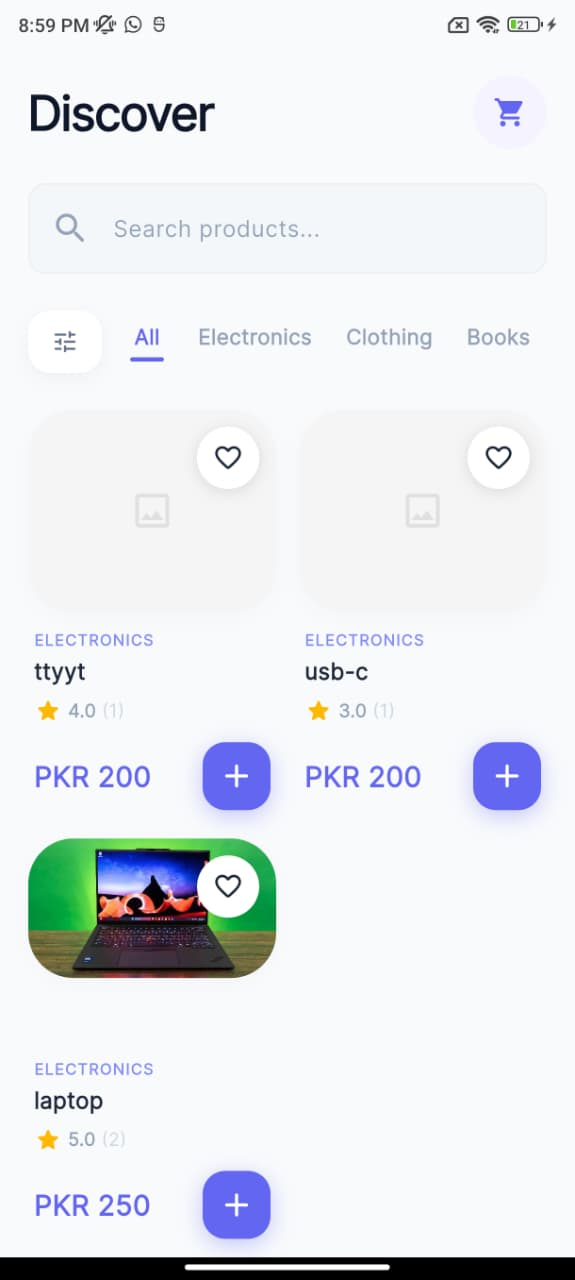
\includegraphics[width=0.3\textwidth]{figures/pictures project/frontend/discover.jpeg}
\caption{Product Browse Screen Interface}
\label{fig:product_browse_screen}
\end{figure}

The product browsing screen Figure \ref{fig:product_browse_screen} is a customer-facing screen where customers can browse through the available products within the catalogue. The interface is a combination of a search box, filtering categories, shortcuts to the wishlist, product ratings, price, and the quick add-to-cart buttons in a scrollable design. This design enables the effective product discovery as users can narrow results and perform actions on products right in the listing view. The navigation is designed to be scanned quickly and allow the user to browse through multiple products without having to open each product separately. The tabs of categories assist in grouping the catalogue in familiar commercial groupings, which is particularly helpful as the marketplace expands. The search query also facilitates the specific product search when the user is aware of what they want to buy. Visual product cards strike a balance between commercial data like price and rating and actionable controls, like the add-to-cart button. This minimizes the purchasing process and enables the customer to speed up his/her discovery to choice. The page is also conducive to exploratory behaviour with several choices in a small yet readable format. Consequently, it serves as the main catalogue interface to provide convenient browsing and make purchases in advance.

\begin{figure}[H]
\centering
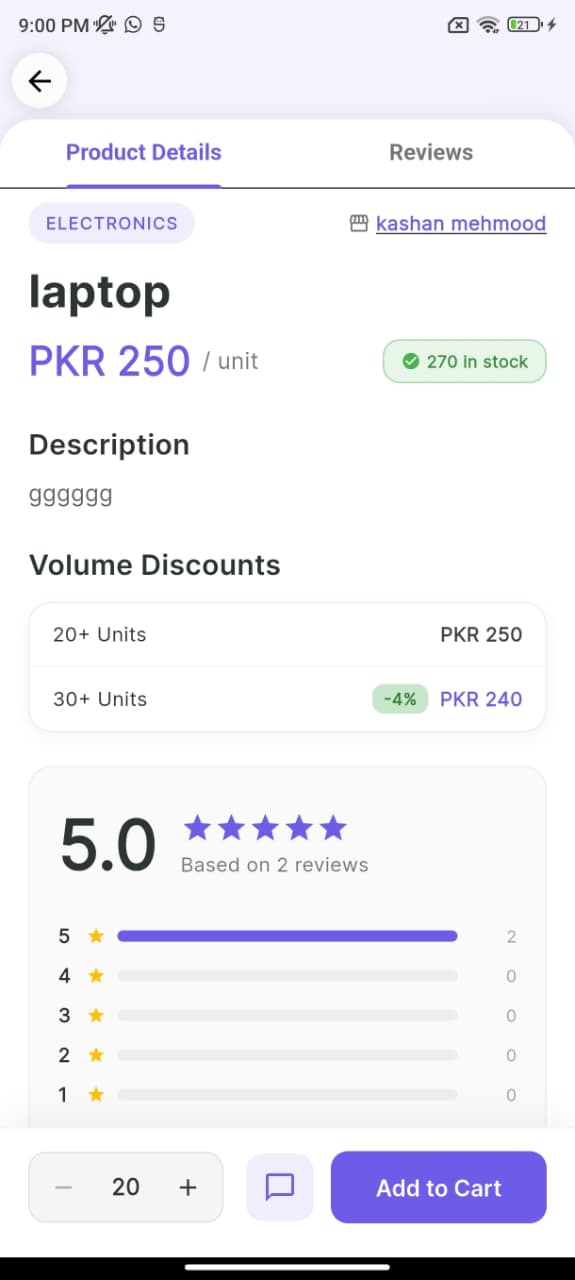
\includegraphics[width=0.4\textwidth]{figures/pictures project/frontend/product description.jpeg}
\caption{Product Detail Screen with Tiered Pricing Interface}
\label{fig:product_detail_screen}
\end{figure}

The product detail screen is shown in figure \ref{fig:product_detail_screen} where the customer has the opportunity to view all the information about the item before buying. The interface displays the category and seller of the product, stock, description, quantity selection, customer review summary and the tiered pricing table which increases or decreases the value based on the volume of bulk purchases. It also gives direct actions to start a chat with the seller and add the number of items chosen to the cart. This is a crucial screen especially in a B2B situation since it is in such a case that buyers require more commercial information before they commit to an order. The availability symbol and the seller identification assists in creating trust and buying confidence. One of the fundamental marketplace features is relayed through the volume discount section which displays the price change with the increase in the quantity of an order. The summary of the reviews also helps make a decision, bringing out the feedback of the collective customers on the same screen. The quantity and persistent action buttons ensure that the purchase process is as near to the product description as possible, without having to navigate further. This screen is the prime point of conversion in the direct-purchase journey by integrating evaluation, communication, and preparation of transactions in a single display. It is thus one of the most densely functional and business important interfaces in the system.

\begin{figure}[H]
\centering
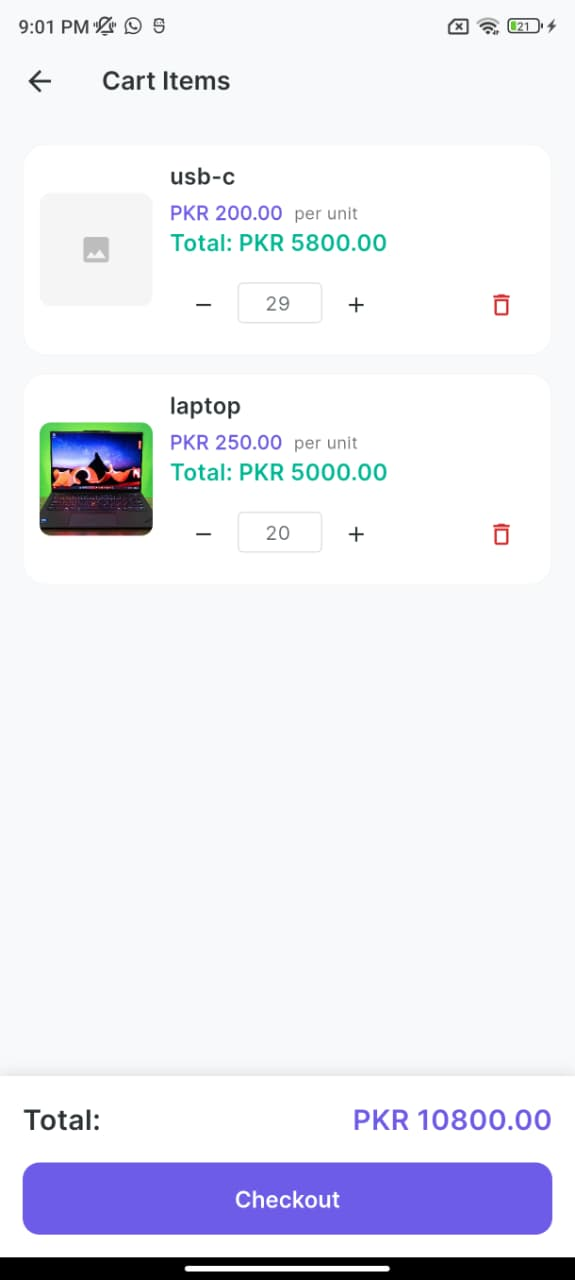
\includegraphics[width=0.3\textwidth]{figures/pictures project/frontend/cart items.jpeg}
\caption{Cart Screen Interface}
\label{fig:cart_screen}
\end{figure}

The cart screen in Figure \ref{fig:cart_screen} is used to gather the selected items prior to checkout. The interface displays all items in the products list their unit price, quantity adjustments, subtotal and remove feature and a running total displayed at the bottom of the screen. Such a design allows the customers to easily alter the quantity of orders and analyze the financial consequences of bulk orders prior to ordering them. The cart is a transient holding space that assists the customers in narrowing down on the decisions they are likely to make in making their purchase decisions prior to making any payments. The controls of quantity increment and decrement are used to facilitate real-time adaptation of order size which is particularly applicable when tiered pricing affects the overall prices. Table of per-item totals and the overall total enhance financial transparency and minimize uncertainty in the process of buying. The capability to delete items in the cart assists the user to have control over what they would like to order. Since the cart can group several products into a single list to be reviewed, it also facilitates the buying patterns of multi-item, which are typical of wholesale. The checkout button is placed as the next most important button and it allows one to be sure that the user will proceed to finalising the order. In general, this screen combines choice of products and formality processing of order in an effective manner.

\begin{figure}[H]
\centering
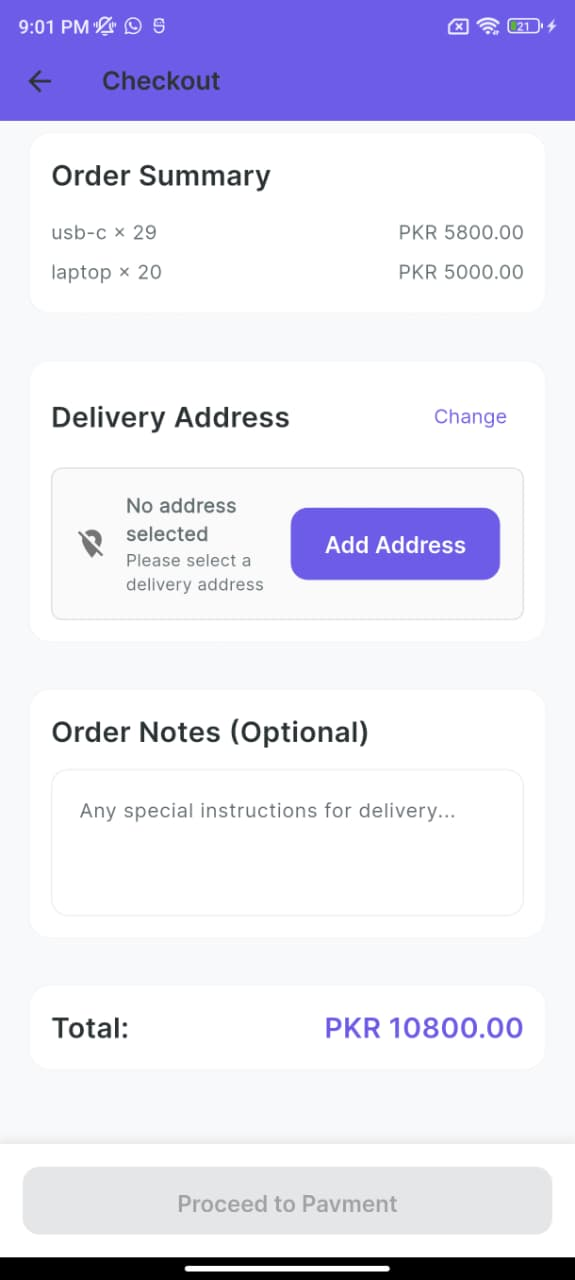
\includegraphics[width=0.4\textwidth]{figures/pictures project/frontend/order summary.jpeg}
\caption{Checkout and Payment Screen Interface}
\label{fig:checkout_screen}
\end{figure}

Figure \ref{fig:checkout_screen} shows the checkout screen that is used to complete an order. It summarises the chosen products, gives the user an opportunity to select or add an address in which to deliver the goods, gives them room to add optional delivery notes, and shows the amount they should pay. The screen serves as the last inspection point prior to the customer being taken through the safe payment channel. Practically, this interface would gather all the vital details of the order that have to be verified prior to the initiation of payment. The delivery address section plays a crucial part in particular since B2B transactions tend to require proper logistics information and destination management. Special instructions, optional notes allow flexibility, and could involve packaging, handling, or contact options. The segregation of order summary, address selection and note generates a systematic flow that minimizes chances of information omission. The placement of the total amount also helps to instill cost consciousness prior to payment verification. It is thus a usability checkpoint, as well as a data-validation step that will help in maintaining order accuracy. It is at the core of converting a shopping cart into a purchase request.

\begin{figure}[H]
\centering
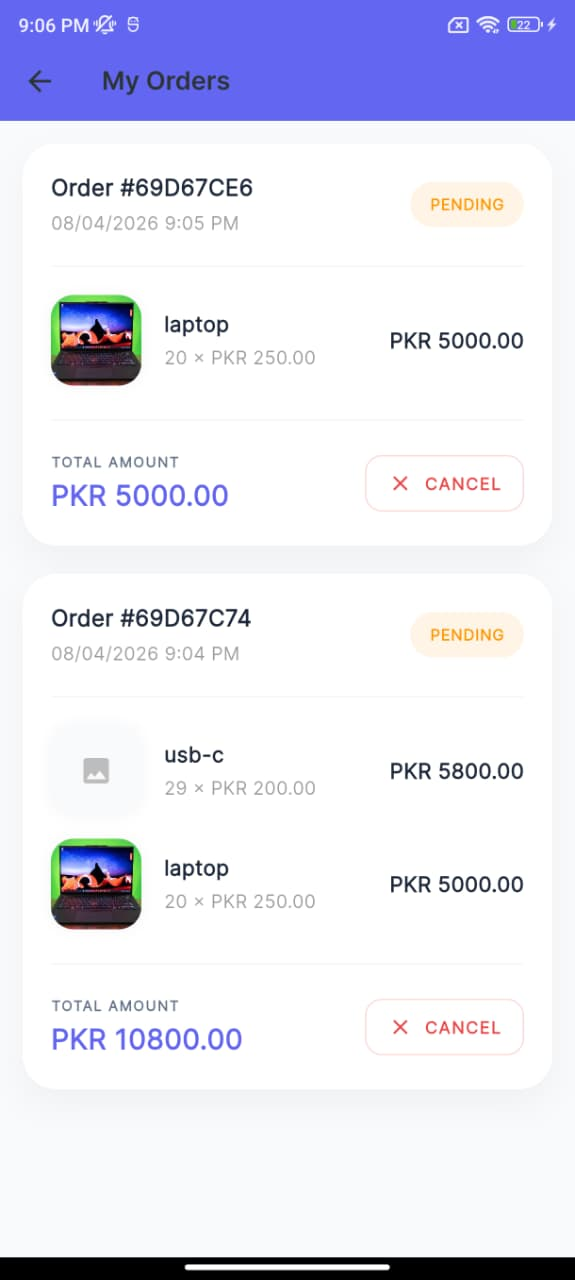
\includegraphics[width=0.4\textwidth]{figures/pictures project/frontend/my orders.jpeg}
\caption{Customer Orders Screen Interface}
\label{fig:orders_screen}
\end{figure}

The customer orders screen is shown in Figure \ref{fig:orders_screen} where the customer can view orders that have been placed in the past. The order cards show the order identifier, time, goods included, price, and processing status, and have the option to cancel orders (where possible). This screen enables the customers to have a clear picture of the history of purchase and the progress of their orders. The interface will also enhance transparency following payment with transaction records remaining transparent and easy to understand. The identifiers of order and timestamps assist users in distinguishing between several purchases and aid in the further reference in communication or dispute resolution. Status labels give a simple impression of the current stage of each order in the fulfilment lifecycle, pending confirmation to delivery. The item previews are also included to make the users remember the contents of every order without necessarily viewing the more detailed screens. This comes in handy especially in repeat-purchase environment where a customer might have a number of overlapping transactions. Canceling orders (where possible) provides the consumer with an added perceptions of control and flexibility. In sum, the orders screen assists in instilling confidence in the customers after purchase and continued management of the relationship between the customer and seller.

\begin{figure}[H]
\centering
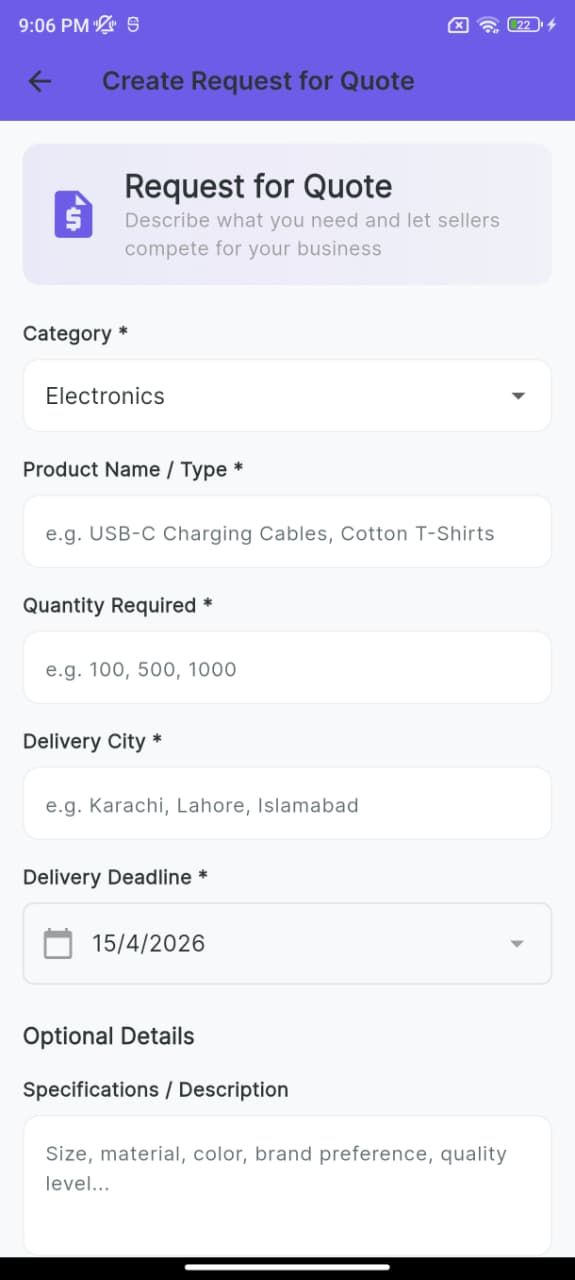
\includegraphics[width=0.4\textwidth]{figures/pictures project/frontend/request for qouta.jpeg}
\caption{Create RFQ Screen Interface}
\label{fig:create_rfq_screen}
\end{figure}

The creation form of quotation-based procurement is the RFQ creation form as shown in figure \ref{fig:create_rfq_screen}. The interface records the category, type of products, quantity needed, city of delivery, deadline and optional specifications in order to ensure that the customers indicate bulk or tailor-made purchasing requirements in a formal format. The design allows sellers to provide specific and competitive quotations. The RFQ workflow stands out as a differentiator of the marketplace since it goes beyond the fixed-price catalogue buying. The structure of the request of the customer in the form of specific fields guarantees the sellers that they will have sufficient information to make realistic offers. These are especially the delivery deadline and the destination in the context of commercial negotiations since they affect the cost, the feasibility and the anticipated lead time. The optional description fields also allow the customer to have some flexibility in describing what they want in quality, materials, or other desired attributes that were not easily available in standard product listing. The interface thus accommodates multi-faceted procurement situations that are prevalent in B2B trade. Its data format is organized and enhances the quality of data as well as the comparability of responses among sellers. This screen is efficient in converting customer demand into a formal marketplace opportunity that could be analyzed and responded to by a number of sellers.


\begin{figure}[H]
\centering
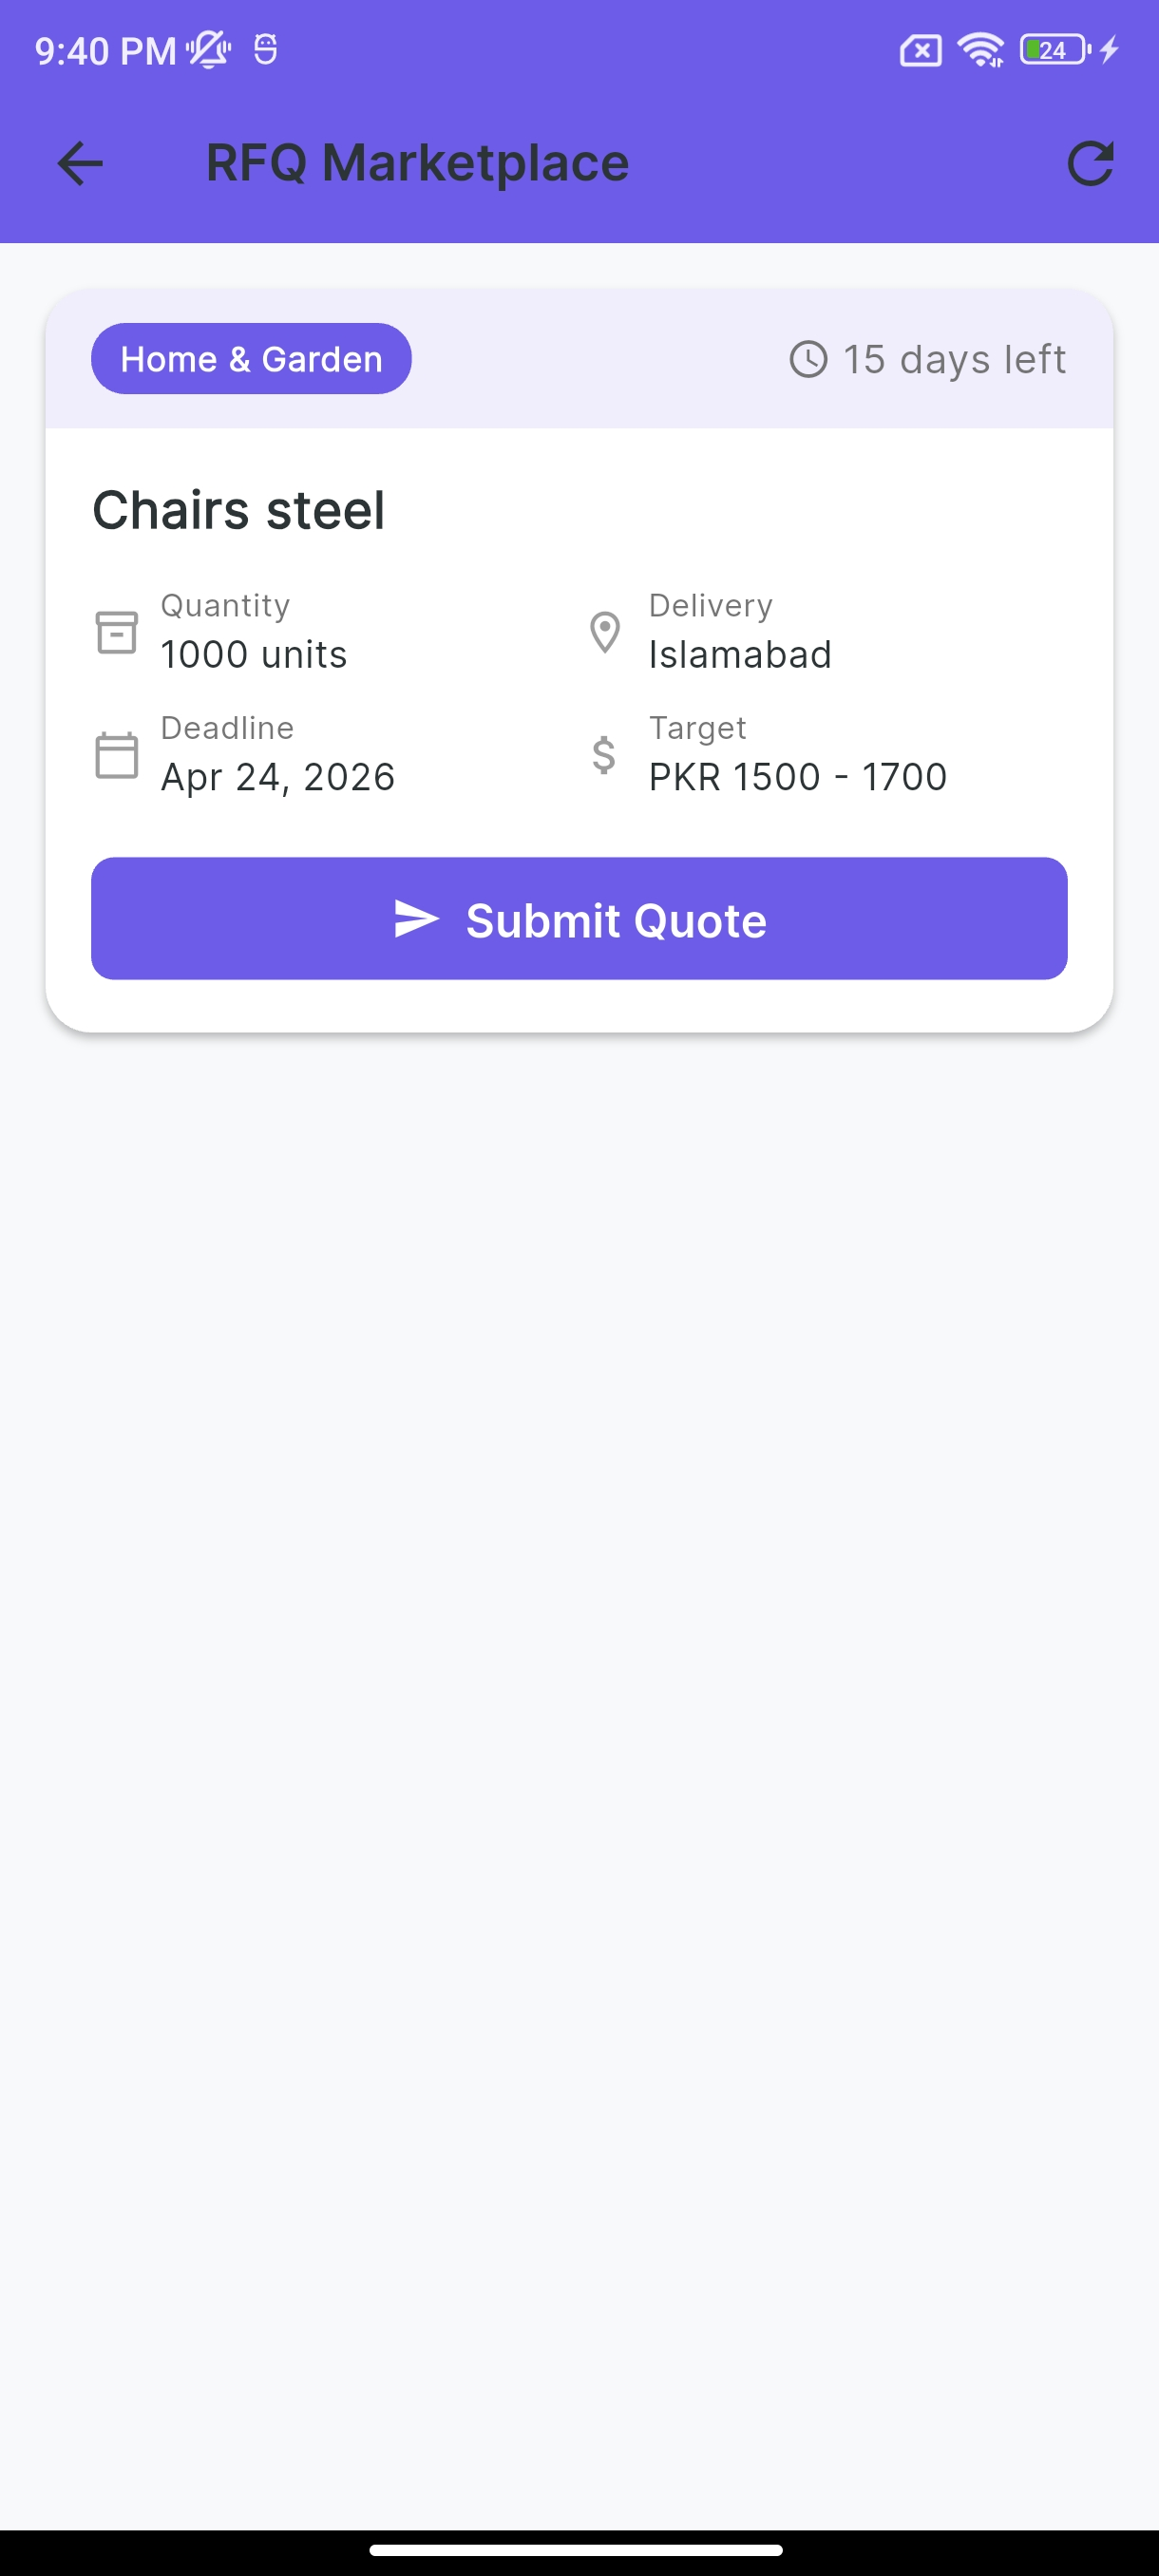
\includegraphics[width=0.4\textwidth]{figures/pictures project/sellerside/rfq market place.jpeg}
\caption{Open RFQ Marketplace Screen Interface (Seller View)}
\label{fig:open_rfqs_screen}
\end{figure}

Figure \ref{fig:open-rfqs-screen} shows the seller-side RFQ marketplace. The RFQ cards contain an overview of the request type, quantity, delivery address, due date and the approximate budget limit, and a direct quote-submission action. The interface enables sellers to find business opportunities they are interested in by aggregating open requests into a single marketplace. This screen will serve as a competitive demand board on which sellers will be able to scan on the open procurement requests and determine which business opportunities can be used in accordance to their inventory and business objectives. The card layout is summarised allowing quick comparison of various RFQs without having to navigate to different pages. Attributes that are of commercial interest like deadline and target budget assist sellers to prioritize the requests that have likelihood of turning into profitable deals. The direct submission cutoff also reduces the response cycle and promotes the participation of sellers in time. Such responsiveness is essential in a multi-seller marketplace to have an ecosystem of active quotations. The screen thus facilitates the opportunity discovery as well as transactional efficiency. It also shows how the platform goes beyond the traditional browsing by providing request-based commerce.

\begin{figure}[H]
\centering
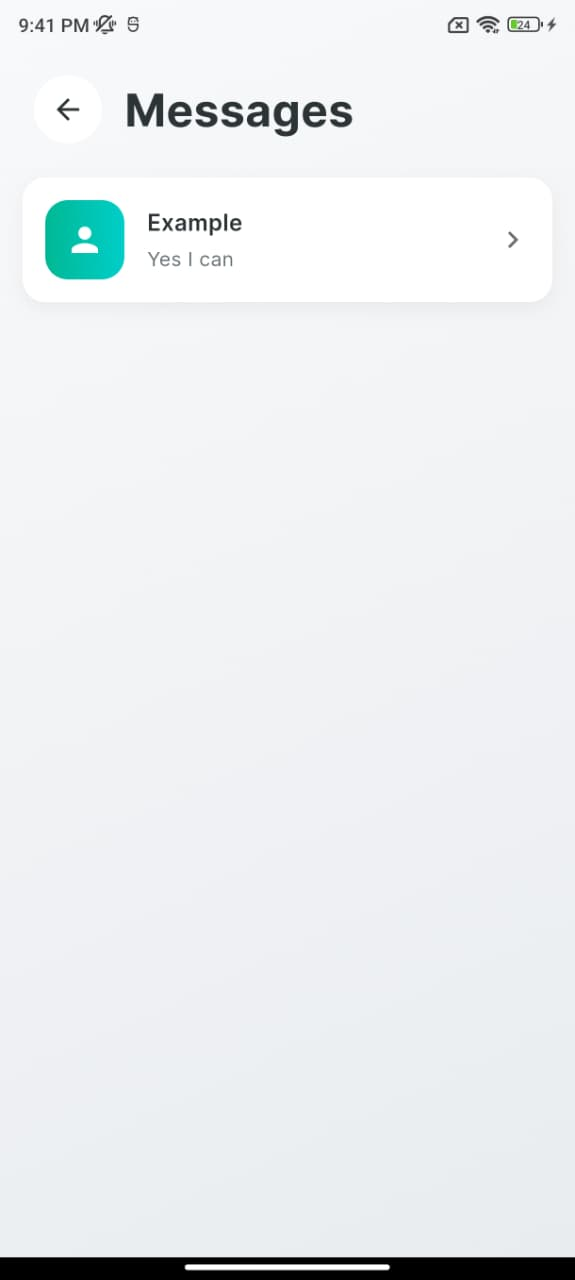
\includegraphics[width=0.4\textwidth]{figures/pictures project/sellerside/messages.jpeg}
\caption{Real-Time Chat Screen Interface}
\label{fig:chat_screen}
\end{figure}

Figure \ref{fig:chat_screen} is the messaging interface that is used to communicate between customers and sellers. The conversations are presented in a straightforward list format with the identity of the participants and the last message preview, and users can easily access current conversations. This screen aids the real-time interactive nature of the platform in clarifying products, orders and RFQ details. The communication is a necessity in the B2B trade, where the buyer and supplier frequently need to discuss quantities, verify specifications, or clarify the questions of fulfilment. The list-based form provides the user with a brief idea of the conversations taking place and allows them to easily locate the latest interaction. The preview of the latest message will enhance message-triage as the user will be able to gauge the relevance of a conversation even before opening it. The minimal design also makes the interaction lean and fits well in the common usage on mobile phones. Messaging imparts as a part and parcel of the marketplace; therefore, users do not have to switch to alternative means of communication. This reinforces a continuity between browsing, placing orders, RFQ management and post sales assistance. Consequently, the chat interface is a key to the responsive commercial coordination of both user roles.
\begin{figure}[H]
\centering
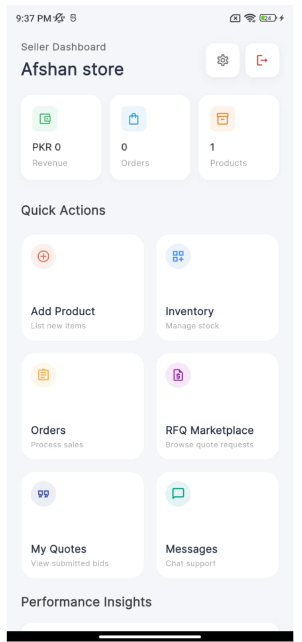
\includegraphics[width=0.4\textwidth]{figures/pictures project/sellerside/seller store.png}
\caption{Seller Home Screen Interface}
\label{fig:seller_home_screen}
\end{figure}

Figure \ref{fig:seller_home_screen} depicts the seller dashboard which is the key control panel of operations on the supplier side. It shows summary data like revenue, order count, products count, and offers fast actions to add products, inventory management, orders, RFQ review, and message review. This job-specific dashboard assists sellers to operate the activity of the marketplace at one point of entry. Operationally, the dashboard simplifies the process of working with sellers as it consolidates the key business functions on a single overview page. The summary cards enable sellers to quickly check their current performance without having to open numerous management screens. Quick-action tiles reduce the time taken in navigation and simplify repetitive processes, like updating inventory or reviewing orders. It is especially useful in a marketplace situation where sellers might be required to act fast in regard to the orders and quotation requests received. The dashboard also indicates the professional identity of the seller account, as the focus on the information regarding revenues and fulfilment is prioritised over consumer-centric browsing metrics. Its design thus favors both the operational consciousness and quick response. In general, it is the primary working environment of participation in a marketplace on the seller side.


\begin{figure}[H]
\centering
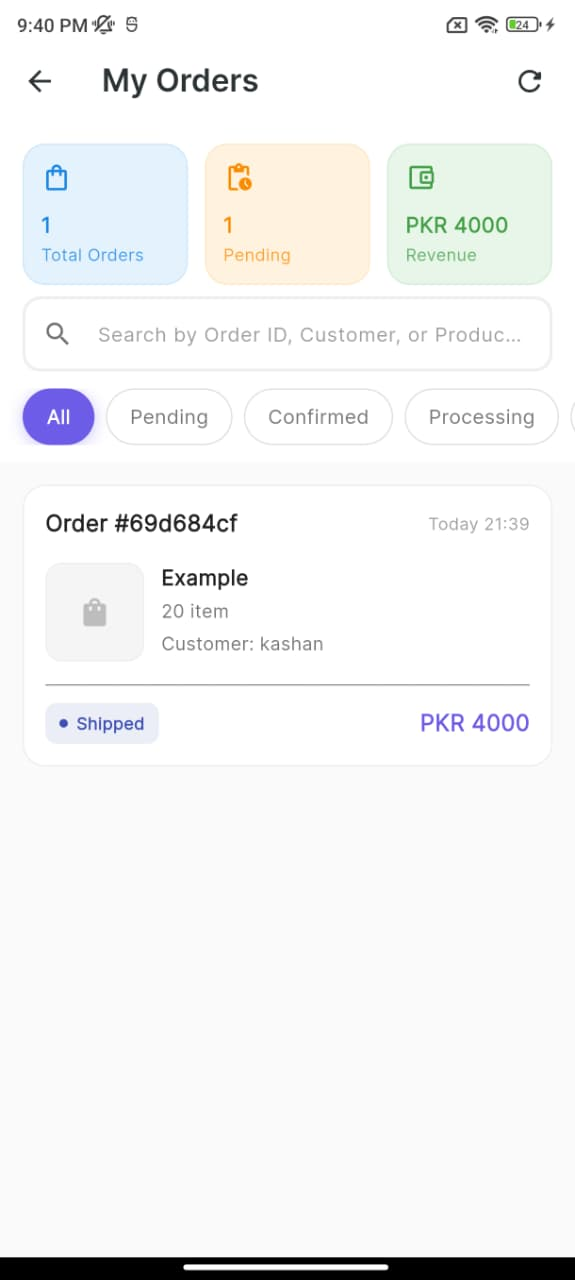
\includegraphics[width=0.4\textwidth]{figures/pictures project/sellerside/my orders.jpeg}
\caption{Seller Orders Management Screen Interface}
\label{fig:seller_orders_screen}
\end{figure}

The seller orders management screen is shown in figure \ref{fig:seller_orders_screen}. The interface provides overview of operating statistics, allows search and status-based filtering, and displays customer orders and item details, buyer details, order status and order value. It is created to assist sellers in monitoring progress in fulfilment and it also allows them to take orders effectively. The screen is customized to fulfilment management whereby sellers must track the flow of transactions and react based on the status of each order. Search and filter controls enhance scalability, because sellers can find particular orders in a short time, despite the growing volume of transactions. The presence of customer identity and item information in every order card facilitates quick decision-making in operations without having to change the pages all the time. Status visibility is particularly crucial since duties of the sellers vary with changes in the state of orders between pending and confirmed, shipped, and delivered. The situational awareness is also enhanced by the operational summary at the top of the screen that sums up important indicators related to orders. This interface thus integrates monitoring, filtering and preparation of actions in one management space. It is at the core of ensuring stable quality and punctuality in seller service.


\begin{figure}[H]
\centering
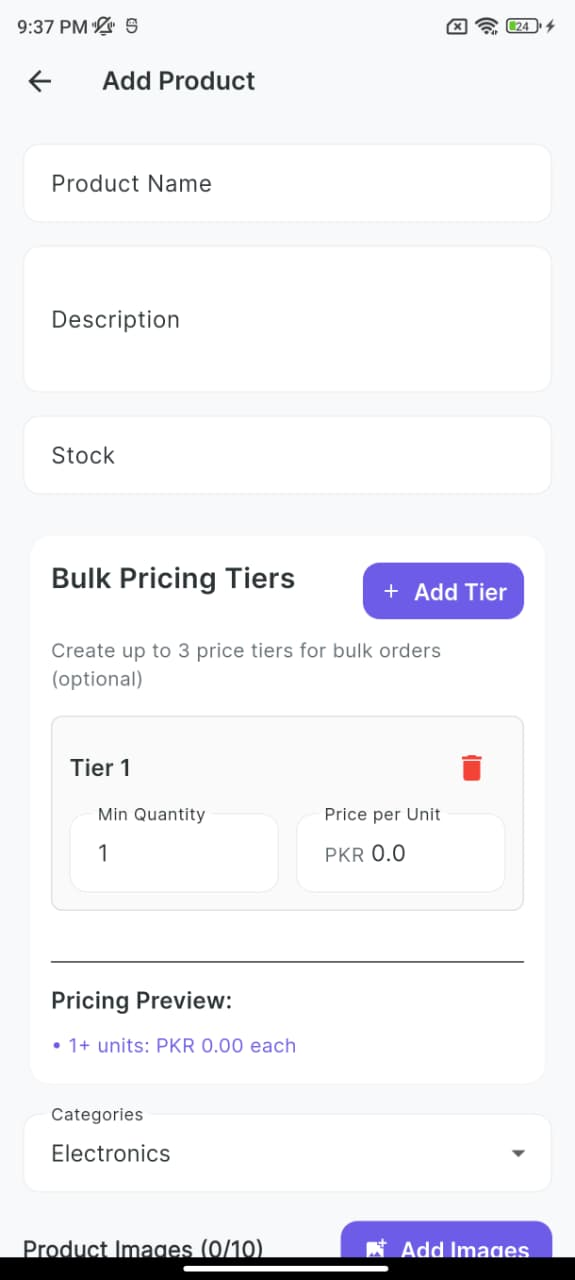
\includegraphics[width=0.4\textwidth]{figures/pictures project/sellerside/add products.jpeg}
\caption{Add Product Screen Interface (Seller)}
\label{fig:add_product_screen}
\end{figure}

The seller product creation interface can be seen in Figure \ref{fig:add_product_screen}. The form also has the product name, description, stock level, category, images and bulk pricing levels which enable the sellers to establish the normal pricing rules and volume-based pricing rules. This screen is crucial in sustaining a catalogue which is specific to wholesale and B2B buying behaviour. It is a form created to encompass a descriptive and a commercial part of a product within a single workflow. Fields like stock quantity and category will make sure that the products are displayed in the same way, and buyers can be able to find them correctly. This feature of the marketplace allowing the introduction of bulk pricing levels directly into the same interface emphasizes the fact that the marketplace supports the idea of commercial negotiations based on quantity. The ability to upload pictures also enhances the presentation of the products because the sellers can communicate the visual quality and the look of the products. The interface reduces the amount of effort needed to publish and manage inventory by putting all these features in a single screen. This plays a role in the involvement of sellers, as simple product creation will motivate a more abundant and lively marketplace catalogue. Effectively, the add-product screen fulfils the role of a seller as a supplier in the digital marketplace.

\begin{figure}[H]
\centering
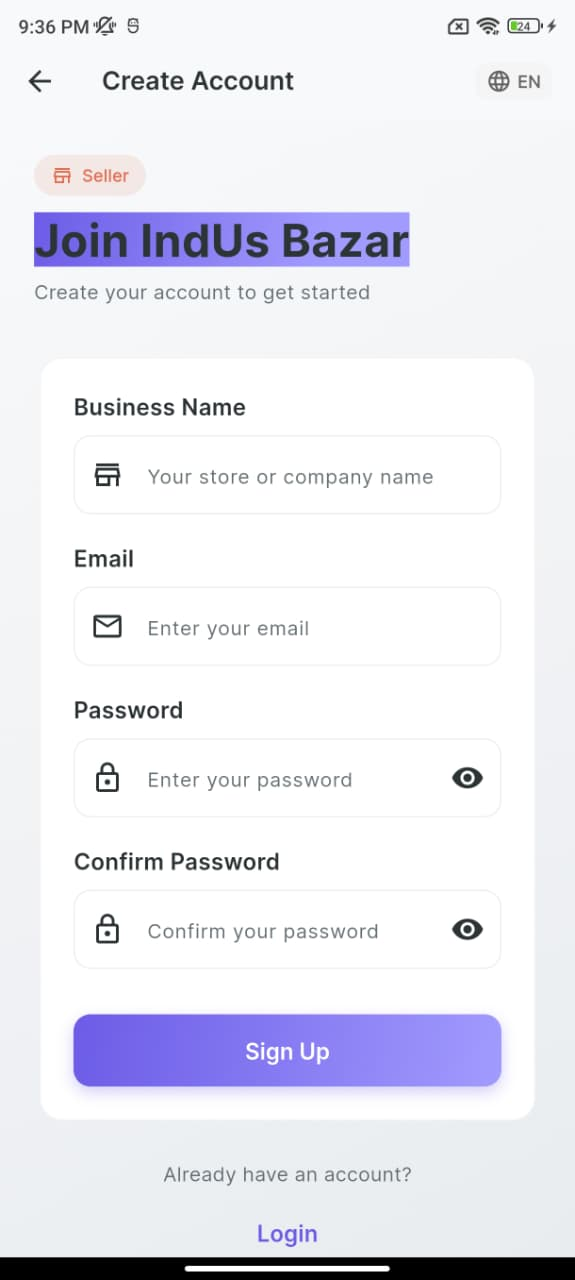
\includegraphics[width=0.4\textwidth]{figures/pictures project/sellerside/create account for seller.jpeg}
\caption{Seller Registration Screen Interface}
\label{fig:seller_profile_screen}
\end{figure}

The seller registration screen is depicted in figure \ref{fig:seller_profile_screen}. The interface gathers business name, email address, password and password confirmation with a clear indication that the account is a seller account. This role-specific onboarding perspective guarantees that the suppliers are introduced into the market by a special registration process. This interface, compared to the conventional customer registration, focuses more on business identity as opposed to personal identity, which is the nature of seller participation. The explicit seller label makes it less ambiguous and assists in aligning the expectations of users at the time of creating an account. It should be consistent with the overall authentication design so as to maintain familiarity yet make the supplier role visually distinct. This role division is significant in that, seller accounts subsequently access specialised dashboards and management tools that buyers do not have access to. The form is clean, which means that it also contributes to fast completion and ease in verifying the needed information. The screen helps to classify accounts correctly and control access by taking suppliers through a different onboarding route. It is thus a significant initial phase of the seller lifecycle in the platform.

\begin{figure}[H]
\centering
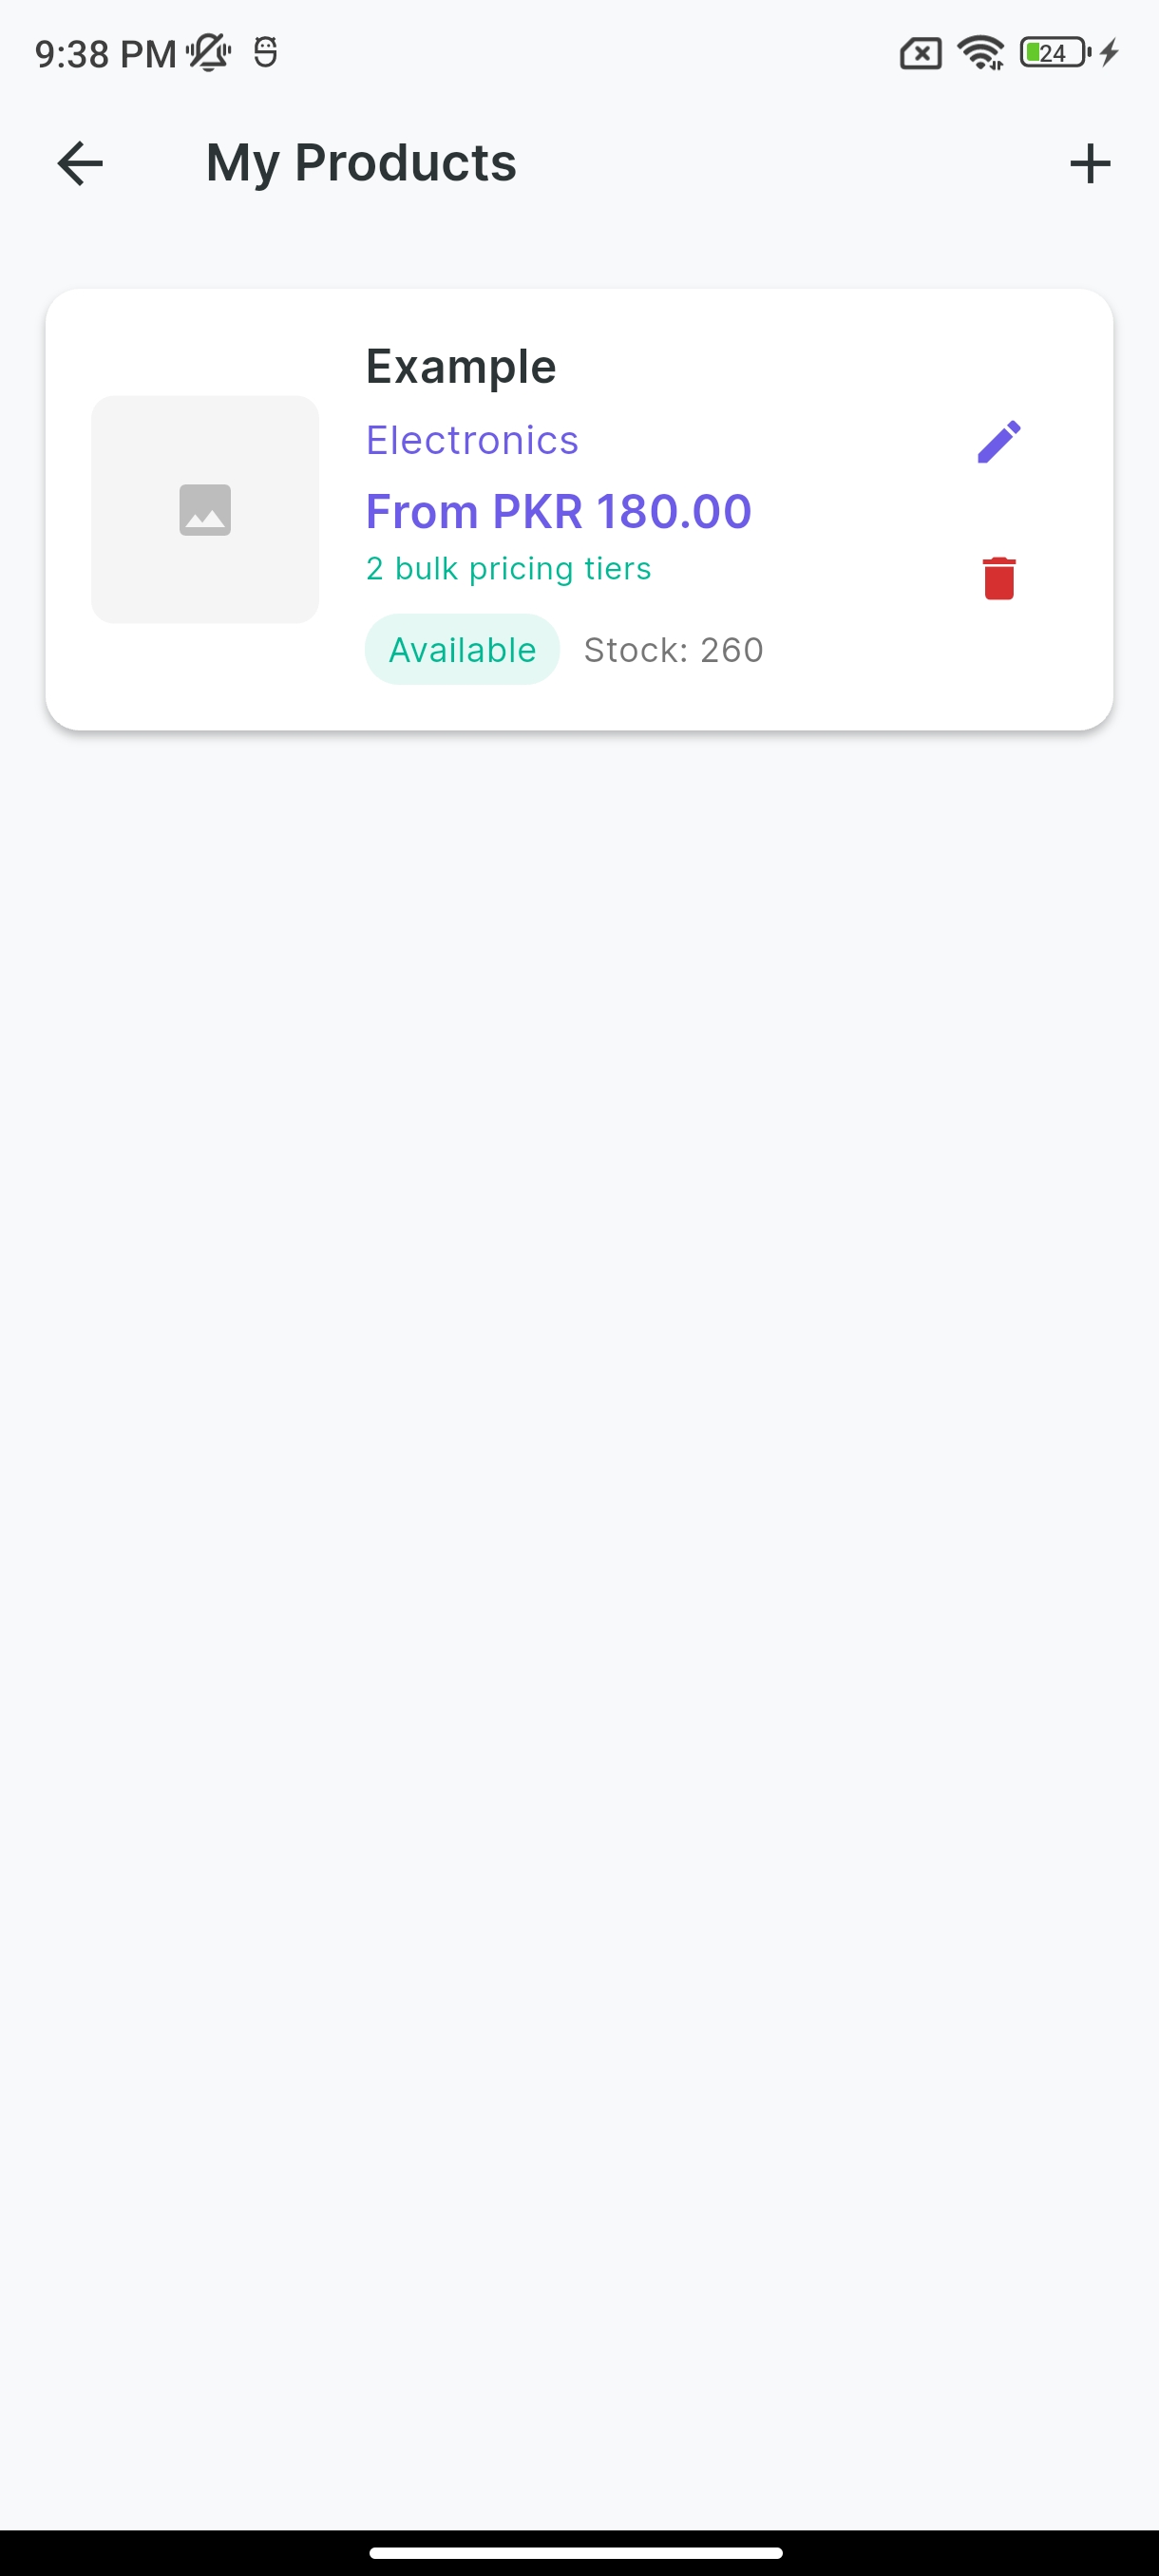
\includegraphics[width=0.4\textwidth]{figures/pictures project/sellerside/my products.jpeg}
\caption{My Products Screen Interface}
\label{fig:admindashboard2}
\end{figure}

The product listing screen of the seller is displayed in figure \ref{fig:admindashboard2}. It shows the items that have already been added by the seller in a tabular format to enable catalogue entries to be checked and edited effectively. This screen helps in the continued maintenance of the storefront inventory of the seller. After publishing products, sellers require an efficient method of checking their catalogue to ensure that their listings are correct and that they are live. The screen fulfils this role by sorting the items on display into a more management-friendly presentation as opposed to a customer-focused one. This type of listing interface can be employed to monitor stock display, pricing confirmation, and to determine products that might require modification or elimination. It also makes repetitive administrative works easier because it provides sellers with an overview of their merchandise. With a dynamic market place, buyers need to trust the product and make transactions, thus its quality and correctness is paramount. This display thus helps in catalogue governance on the seller side. It serves as an internal product browsing experience that corresponds to the external product browsing experience.

\begin{figure}[H]
\centering
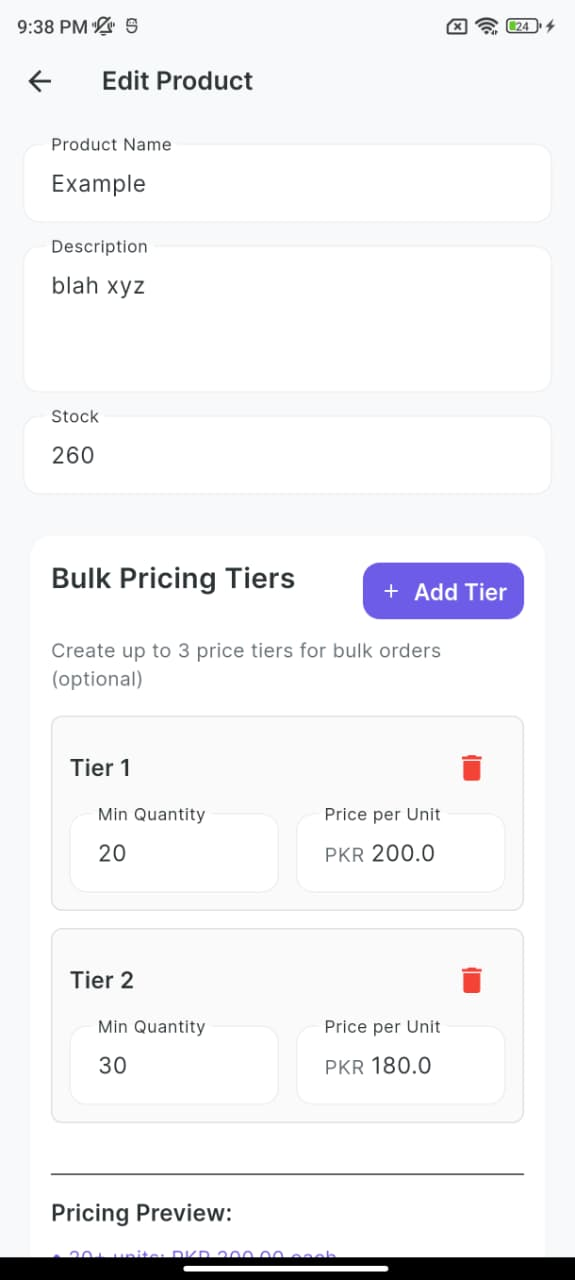
\includegraphics[width=0.4\textwidth]{figures/pictures project/sellerside/edit products.jpeg}
\caption{Edit Product Screen Interface}
\label{fig:admindashboard3}
\end{figure}

Figure \ref{fig:admindashboard3} displays the product editing screen that sellers use to edit existing listings. Using this interface, sellers have the ability to update product attributes, pricing details, among others without the need to create a new record. This enhances the flexibility of the catalogue and makes product maintenance easy. Editing of products once they are created is significant since commercial information tends to vary with time, particularly in competitive wholesale set-ups. As the market conditions vary, sellers might be required to change the prices, descriptions, stocks, or to fix the listing errors. The continuity of an existing product record is maintained by having an editing interface, and operational updates are easily made. This minimises duplication of the database and needless recreation of catalogue records. Usability wise, it also reduces maintenance effort as it maintains the tasks of modification in a familiar form based environment. The screen thus aids in data consistency, catalogue accuracy and responsiveness of the sellers. It is directly related to the sustainability of the marketplace inventory.

\begin{figure}[H]
\centering
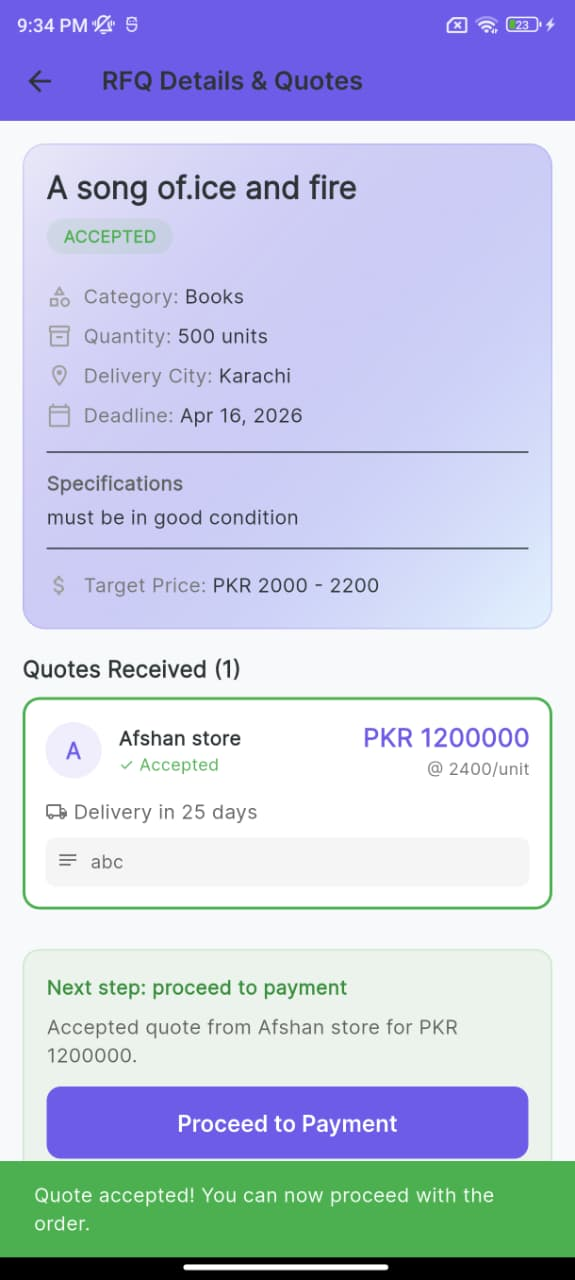
\includegraphics[width=0.4\textwidth]{figures/pictures project/sellerside/rfq details.jpeg}
\caption{RFQ Details Screen Interface}
\label{fig:users}
\end{figure}

As shown in figure \ref{fig:users}, the RFQ details screen is as shown by the seller side. It reveals the information on quotation requests by the customer in a detailed manner, which enables the seller to examine the requirements prior to writing a commercial response. This screen assists in making informed and correct quotation preparation. In B2B procurement, the quality of the submitted quote directly depends on the skills of a seller to interpret customer needs in the appropriate manner. Detailed view is thus important since it offers the entire picture of the request instead of a summary of the marketplace. Quantity, delivery location, target price expectation and descriptive requirements are some of the information that can be used by the seller to determine feasibility and trade-level viability. Such a more detailed background diminishes the possibility of unrealistic or partial quotes. It also gives the seller the capability of matching the offer made with the expectations and operational limitations of the customer. This screen enhances the quality of negotiation in the platform by acting as an analytical step prior to submitting a quote. It is thus an important support interface to the RFQ process.
\begin{figure}[H]
\centering
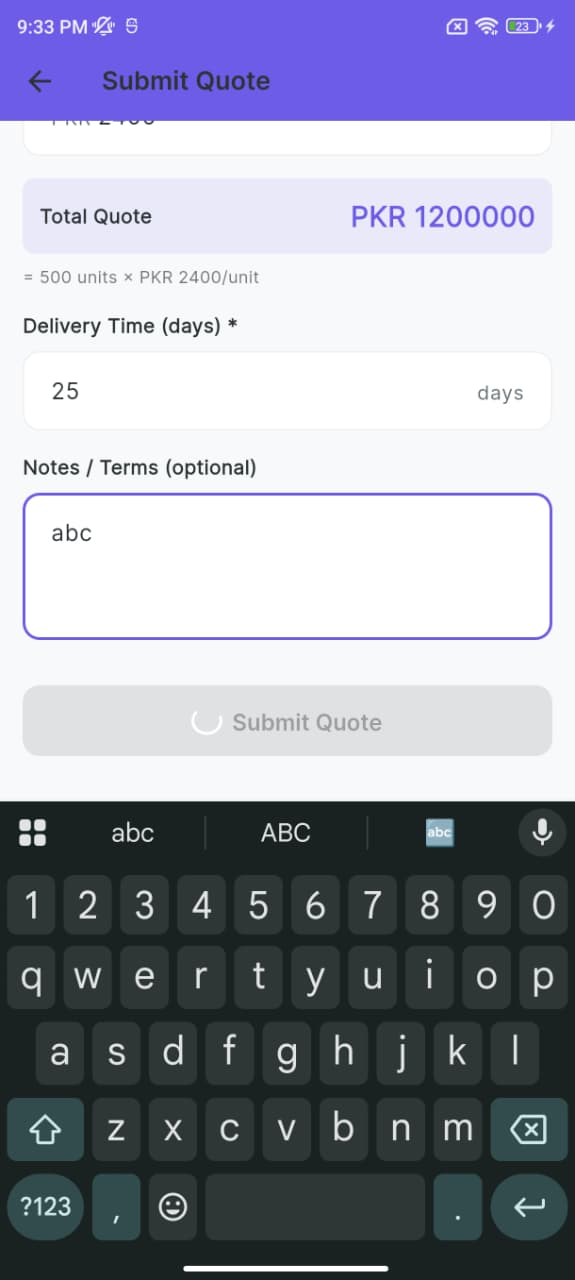
\includegraphics[width=0.4\textwidth]{figures/pictures project/sellerside/submit qouta.jpeg}
\caption{Submit Quote Screen Interface}
\label{fig:appointments}
\end{figure}

Figure \ref{fig:appointments} illustrates the quote submission interface that sellers use in response to an RFQ. The screen records the quoted price, delivery schedule and any notes or conditions that are optional allowing the seller to make a full offer to the requesting customer. It is an important component of the quotation-based negotiation process. The interface will convert the intent of the seller into a structured commercial proposal, which can be assessed by the buyer. The incorporation of the financial and logistical sphere allows preparing the offers in a more realistic and practical manner than a bare price-only response. Optional notes provide sellers with space to provide information about assumptions, terms, or details of the services that can be considered during acceptance. The fact that there is a final submission action makes the quotation process in the system formal. Process wise, this screen will translate RFQ review to a tangible marketplace response. It also normalises the formatting of quotes among the sellers and this simplifies comparison among buyers. By doing so, the screen will not only add value to the quality of the negotiation but also to the consistency of transactions.


\begin{figure}[H]
\centering
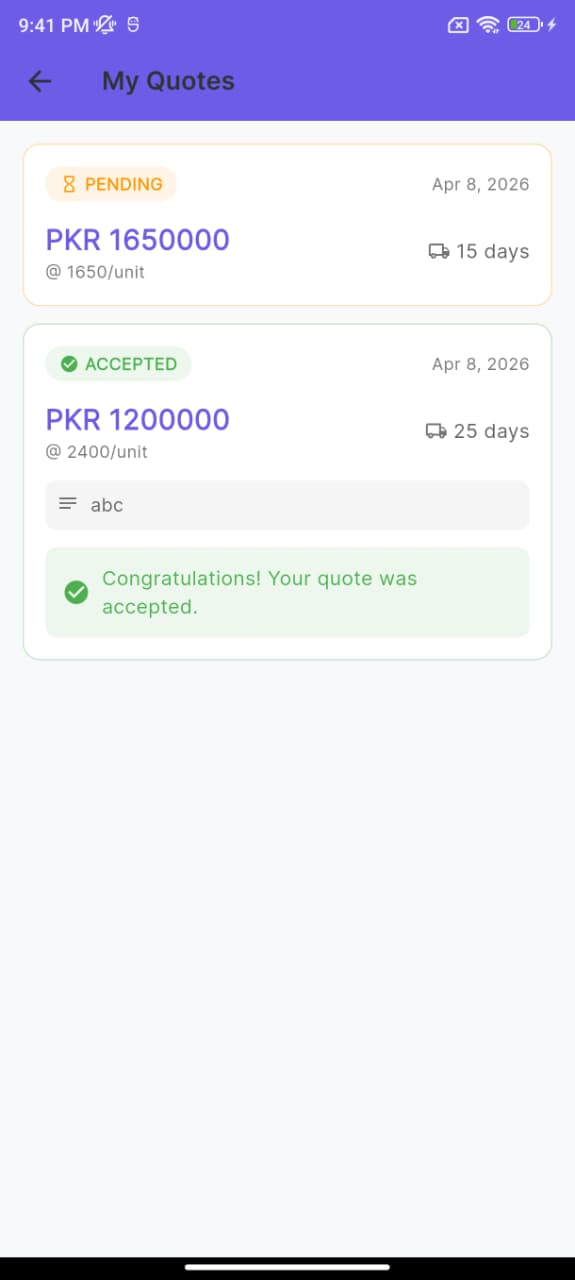
\includegraphics[width=0.4\textwidth]{figures/pictures project/sellerside/my qoutas.jpeg}
\caption{My Quotes Screen Interface}
\label{fig:reports}
\end{figure}

Figure \ref{fig:reports} shows the seller quotes screen, with all quotations submitted in the past, able to be viewed in a single location. This interface assists the sellers to track their bids and track quoted opportunities at the market. It enhances transparency of the seller involvement in the RFQ. Once quotes have been received, the sellers need a clear picture of their pending and past responses so as to be able to control any follow-up measures. The screen offers such visibility, which is to bundle together quotations into one management view. This assists the sellers in knowing how effectively they are working with customer demands and what possibilities they still have. A centralised quote list will also minimise the chances of losing track of already made offers in a busy business environment. In terms of usability, it forms continuity between the discovery of RFQs, the creation of quotes, and subsequent monitoring. This renders the quotation workflow complete as opposed to being fragmented on separate screens. The screen, therefore, plays a significant management role in the bid of the seller.

\begin{figure}[H]
\centering
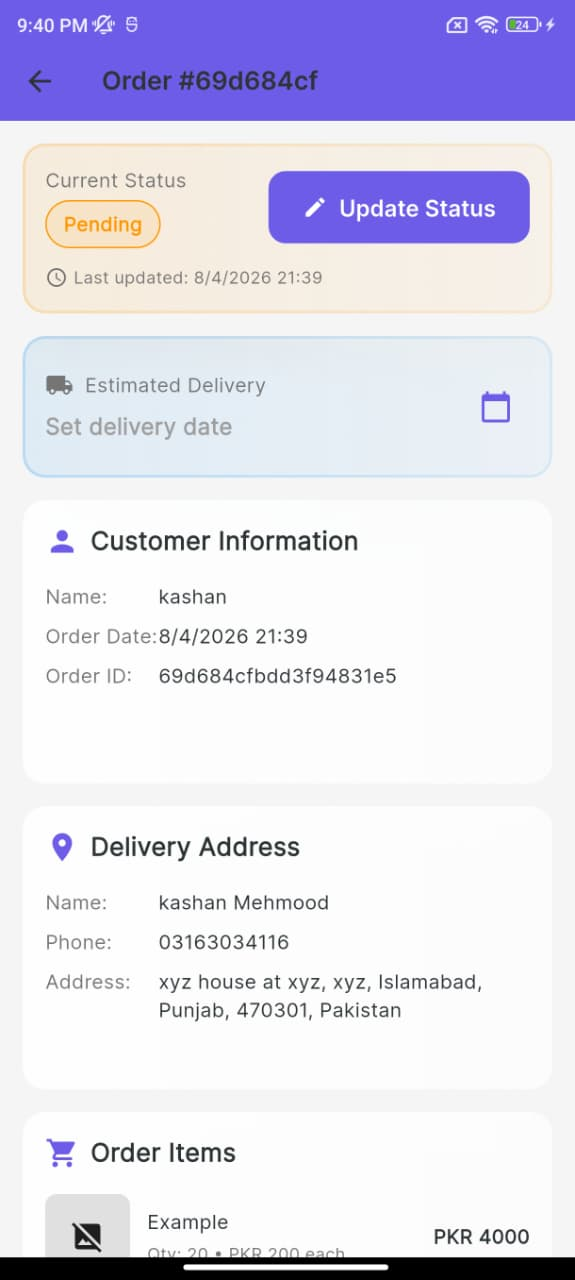
\includegraphics[width=0.4\textwidth]{figures/pictures project/sellerside/order info.jpeg}
\caption{Order Information Screen Interface}
\label{fig:submissions}
\end{figure}

The order information screen shown to sellers is shown in figure \ref{fig:submissions}. It is a more in-depth look at an order, enabling the seller to examine transaction data and information related to fulfilment prior to the next action in the business. This enhances seller-side processing and monitoring of orders. When the seller requires to establish what has been bought, expectations of delivery, or prepare status changes in the order lifecycle, detailed order checking is required. This screen aids those activities by showing an in-depth view of operation compared to the higher order list. The extra data assists in avoiding fulfilment errors and allows making the coordination with customer requirements more efficient. It is also used as a reference point in responding to order specific questions using the messaging channel. Practically, these detail views are very crucial in ensuring that an order is well handled particularly when there are many transactions being handled at once. The screen thus supplements the overall orders management interface by allowing closer viewing and preparedness to action. It has a direct effect on quality of service, accuracy of fulfilment and accountability of the seller.






\chapter{System Implementation} \label{chap:sysImplementation}
%\version{v1.10.2015}

\section*{}
The process of turning an idea into a reality is called implementation. Implementation of a technical specification or an algorithm, in the form of a program or a software component or in any other form a computer system, is the process of programming and deployment. In the case of Indus Bazar, the implementation is the translation of the architectural design of a B2B/B2C marketplace into a fully functioning Flutter-based mobile application backed by a cloud computing server that allows manufacturers, wholesalers, and retailers in the entire country of Pakistan to connect, negotiate, and conduct business in one cohesive digital platform.

\section{System Architecture}

Indus Bazar is designed on a strong 3-Tier Architecture which provides a scalable, maintainable and secure B2B marketplace experience. This design ensures there is a well-defined division of responsibilities at the presentation layer (user interface), application layer (business logic), and data layer (database management). The system enables these components to be independently developed, tested and deployed, which greatly increases flexibility and minimizes the complexity of the system.The presentation layer gives manufacturers and buyers a user-friendly and responsive interface to make user experience cross-user activities smooth. Core functionalities like user authentication, product management, order processing and real time communication regulated by business rules and data consistency are dealt with by the application layer. In the meantime, the data layer safely handles all transactional and user information, facilitating effective storage, retrieval and integrity by optimizing the database design.This layered design improves the performance of the system, enables both horizontal and vertical scaling and improves on security since the layers are limited in direct contact.It also makes future upgrades, addition of new functionalities (including AI-based suggestions or analytics), and maintenance simpler and Indus Bazar a brand of modern B2B commerce in the future.
\begin{figure}[H]
\centering
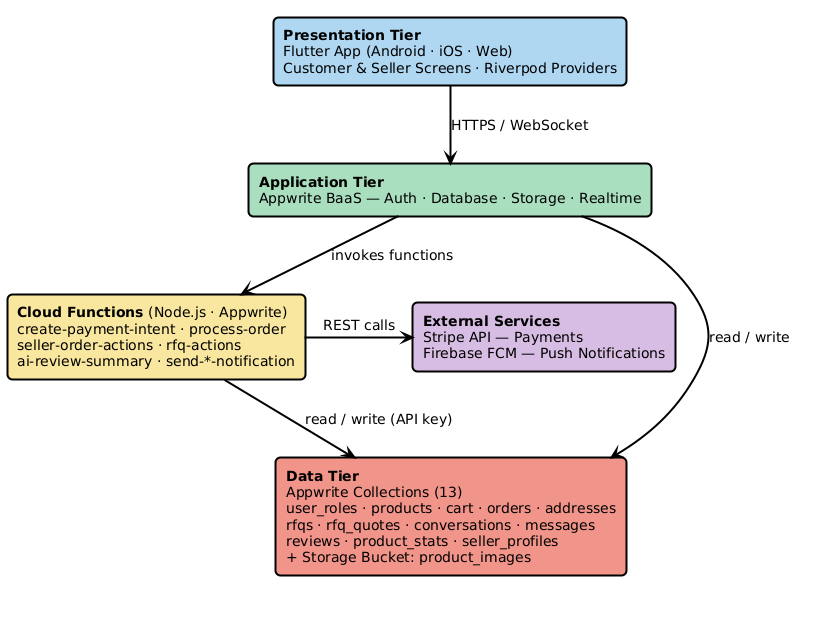
\includegraphics[width=1.0\textwidth]{figures/pictures project/Architecture.png}
\caption{Indus Bazar 3-Tier System Architecture}
\label{fig:system_architecture_implementation}
\end{figure}

The architectural diagram shown in Figure \ref{fig:system_architecture_implementation} depicts the entire 3-level model of the Indus Bazar B2B marketplace. The individual tiers have different functions and they work harmoniously together to provide a cohesive digital commerce platform between manufacturers, wholesalers and retailers in Pakistan.

\subsection{Presentation Tier - User Interface Layer}
Presentation level is the main interaction point between the customers and sellers with the Indus Bazar. This interface is developed with Flutter (Dart), a high-performance, cross-platform mobile application that is natively supported on Android and can be accessed through the web, providing a consistent and user-friendly user experience, no matter the device used.

\subsubsection{Customer Interface Components:}
\begin{itemize}
    \item \textbf{Customer Login Interface:} Customer Login with secure authentications and access to the personalised customer role-based routing with an AppWrapper widget as a dashboard.
    \item \textbf{Product Browse Screen:} Advanced product catalogue category filter, key word search, and treading stacked bulk pricing showcase effective product exploration.
    \item \textbf{Product Detail Screen:} Product in detail with multi-image gallery, full order-based real-time tiered pricing recalculation, specifications and seller information, quantity.
    \item \textbf{Cart and Checkout:} Smoother cart operations with price tier resolving quantity-awareness, address delivery choice, and built-in Stripe payment sheet to secure payments.
   \item \textbf{Order Management:} Full order history and live tracking of status (pending, confirmed, shipped, delivered) with push notification notifications at every lifecycle transition.
   \item \textbf{RFQ Marketplace:} Request for Quotation interface which enables customers to post procurement order, check out competitive seller quotes and take the best offer and move on to payment.
   \item \textbf{Real-Time Chat:} In-built messaging system to communicate directly with the buyer and seller, advertising text and picture messages with live unread badge counters.
  \item \textbf{Intelligent product review interface:} An interface that demonstrates the AI generated summaries of feedback of customers in English and Urdu to be informed in making their purchase decisions.
  \item \textbf{Address Management:} Multi address management screen to enable customers to add or edit their addresses and choose delivery addresses when making the checkout.
\end{itemize}

\subsubsection{Seller Interface Components:}
\begin{itemize}
   \item \textbf{Seller Dashboard:} Headquarters to deal with product listings, track incoming orders, and the reply to proactive RFQ requests in the marketplace.
   \item \textbf{Product Management:} Complete product life cycle management such as add, edit and deactivate multiple image upload and adjustable tiered pricing models.
   \item \textbf{Order Fulfilment:} Status progression controls (confirm, deliver, cancel) and Seller-side order management, and automatic push notifications to the customers at every stage.
   \item \textbf{RFQ Response System:} Open RFQ marketplace view where the sellers can browse the active one, respond to customer requests, provide competitive quotes, and handle orders converted to accepted quotes.
   \item \textbf{Seller Profile:} Business profile management such as business name, city, contact. The information, profile picture, and average customer rating would be shown to all purchasers.
   \item \textbf{Chat Interface:} Live chatting with the customers to explain the specifications of the products, price negotiation, and establish business relationships in the long term, directly on the platform.
    
\end{itemize}

\subsection{Application Tier - Business Logic Layer}
Application Tier involves the business logic of the platform and is where all the operations of the system are coordinated. Developed on a Backend-as-a-Service (BaaS) based on Appwrite and eight Node.js serverless cloud functions, this layer makes sure the communication between the user interface and the underlying data systems is secure and efficient.

\subsubsection{Core Application Modules:}
\begin{itemize}
    \item \textbf{Authentication Service:} Provides secure user registration, enforcement of email verification, session management based on roles, and deep links to password recovery with Appwrite Account APIs and deep link schemes (indusbazar://verify and indusbazar://reset-password).
    \item \textbf{Product Catalogue Engine:} Processes product listings, category searches, search indexes, stock tracking, and tiered price logic, secure bulk price resolution on the basis of order quantity limits set on a product basis.
    \item \textbf{Payment Processing Function (create-payment-intent):} a cloud based on the server-side Node.js function to make Stripe PaymentIntents and Customer objects safely, guaranteeing the Stripe secret key is never sent to the client.
    \item \textbf{Order Processing Function (process-order):} Processes atom order creation, stock de-To avoid overselling under a single server-side transaction, a single server-side transaction is done to induce, and cart clearing concurrent customer orders.
    \item \textbf{RFQ Actions Function (rfq-actions):} The overall RFQ lifecycle includes status transitions (open, quoted, accepted, expired, cancelled), quote submission, quote acceptance.
    \item \textbf{Seller Order Actions:} The Seller Order Actions thing lets sellers list and update the status of orders. They can use an API key to get around the security that's in place for customers. This way sellers can still keep all the data safe.
    \item \textbf{AI Review Summary:} The AI Review Summary thing uses the Google Gemini API to make summaries of what customers are saying. These summaries are in two languages, English and Urdu. The summaries are stored in a place so they can be found quickly.
    \item \textbf{Notification Functions:} There are some functions that send notifications to peoples phones. These functions are called send-order-notification, send-chat-notification and send-rfq-notification. They use Firebase Cloud Messaging to send the notifications in time.
    \item \textbf{Real-Time Chat Engine:} The Real-Time Chat Engine is like a messaging system. It uses Appwrite Realtime WebSocket subscriptions to send messages away. It also updates the count of messages in real time so people can see when they have new messages without having to check all the time.

\end{itemize}

\subsection{Data Tier - Information Storage Layer}
The Data Tier provides secure and efficient data persistence through Appwrite's NoSQL document database and cloud storage, ensuring data consistency, integrity, and availability across all platform operations. This layer manages the complete lifecycle of marketplace data while complying with privacy and security requirements through document-level Row-Level Security (RLS) enforced at the Appwrite platform level.

\subsubsection{Database Components:}
\begin{itemize}
    \item \textbf{user-roles Collection:} This collection contains the mapping between the Appwrite user IDs, which are assigned roles (Customer or Seller), and FCM push notification tokens to deliver targeted notifications.
    \item \textbf{products Collection:} The main product catalogue where the product name, description, classification, inventory levels, status, seller presentations, and levels of price reduction are stored. It supports up to three price levels with minimum quantity limits.
    \item \textbf{cart Collection:} Stores customer cart items connecting user IDs to product IDs with selected quantities, with real-time recalculation of tiers in the checkout flow.
    \item \textbf{orders Collection:} Contains finalized records of orders including customer information and JSON-encoded item arrays (productId, productName, price, quantity, sellerId), amount paid, purchase intent, delivery address, reference address, approximate delivery date, and order lifecycle status.
    \item \textbf{addresses Collection:} Records customer delivery addresses including full name, phone number, street lines, city, province, postal code, and country, along with a default address flag for streamlined checkout.
    \item \textbf{seller-profiles Collection:} Stores seller business profile data such as business name, description, phone, address, city, profile image URL, and a lowercase city field for case-insensitive geographic search.
    \item \textbf{reviews Collection:} The reviews collection contains product review records. These records include a rating from 1 to 5, a title, a comment, image URLs, a flag indicating whether the purchase was verified, a helpful count, and tracking of users who found the review helpful. This ensures the authenticity of reviews.
    \item \textbf{product\_stats Collection:} This collection stores rating statistics for each product. It includes the overall rating, total number of reviews, and the count of reviews for each rating from 1 to 5. This allows efficient display of statistics without real-time computation.
    \item \textbf{conversations Collection:} Stores chat threads. Each thread is identified by the customer ID, seller ID, and product ID. It also includes a preview of the latest message, timestamp, and the number of unread messages for each user.
    \item \textbf{messages Collection:} Stores individual chat messages linked to conversation threads. Each message contains the sender's ID, message text, an image URL, and a timestamp. It also tracks read status and updates for each message.
   \item \textbf{rfqs Collection:} Stores Request for Quotation (RFQ) documents. Each record includes customer ID, product name, category, quantity, delivery city, deadline, specifications, optional target price range, and current status.
   \item \textbf{rfq\_quotes Collection:} Contains quotes submitted by sellers for RFQ documents. It records unit price, lead time in days, notes, and acceptance status.
   \item \textbf{review\_summaries Collection:} Caches AI-generated review summaries. The ai-review-summary cloud function manages these records to reduce API calls to Gemini and improve response times.
   \item \textbf{Appwrite Storage (product\_images):} This storage bucket is used for product catalogue images and review attachment images. MIME types are validated at both the client side and bucket level to ensure file integrity and security.
\end{itemize}
The Indus Bazar platform has a 3-tier architecture that makes it a reliable and intelligent B2B marketplace. This means Indus Bazar is flexible.
Indus Bazar delivers data security, user privacy and commercial performance at a high level.The different parts of the Indus Bazar platform work together to make sure data moves freely.The Indus Bazar platform responds to what each user needs. It does this in real time.This helps Indus Bazar support all the things that need to happen in a B2B marketplace, in Pakistan.

\section{System Internal Components}
There are working parts of Indus Bazar. These sections assist in offering a service between businesses to purchase and sell with one another.Every section has a task to play. This makes the system to work and provides users with an experience.The platform is used by customers and sellers.They receive the potential experience whilst utilizing Indus Bazar.Indus Bazar ensures that it is easily usable by customers and sellers.It assists them to transact business with one another.
\subsection{System Functionality Overview}
The system consists of components that interact with each other. These segments are puzzle segments that will be assembled to give an online shopping system. They collaborate well to provide businesses with a secure and excellent place to market products online. This suits any type of businesses be it the shops or large factories. The system possesses features and is geared towards the people in Pakistan. The system is also secure meaning that it safeguards businesses utilizing it. Pakistani businesses of all sizes can use this system from retailers, to large manufacturers.

\subsubsection{Core Functional Components}

\paragraph{Authentication and User Management System}
Authentication system offers secure access control with industry-standard Appwrite Account APIs. It serves multi-role user registration (Customer and Seller), deep link-based enforcement of email verification, session management and password recovery. The AppWrapper widget constantly checks the authentication and email verification status and does not allow a user to access any dashboard screen until verified. Role assignment gets stored in the collection of user roles as soon as an account is created, and the dashboard can be routed properly, and feature access is granted even during the first login.

\paragraph{Product Catalogue and Search Engine}
This component manages the complete product discovery and management experience, including:
\begin{itemize}
    \item \textbf{Product Listings:} Organized catalogue, categorized, and searchable by keyword to enable effective product discovery within the marketplace.
    \item \textbf{Tiered Bulk Pricing:} Unit price is automatically recalculated according to configured quantity thresholds (volume-based B2B purchases with up to three pricing levels per product), allowing bulk purchasing with transparent pricing.
    \item \textbf{Multi-Image Gallery:} Product images are uploaded to Appwrite Storage and displayed with effective caching to ensure a smooth and fast browsing experience.
    \item \textbf{Seller Product Management:} Sellers can add, edit, and deactivate products with full control over stock quantities, pricing, and product visibility across the platform.
\end{itemize}

\paragraph{Cart and Checkout System}
The cart and checkout module provides a streamlined purchasing workflow from product selection to payment confirmation:
\begin{itemize}
    \item \textbf{Intelligent Cart Management:} Real-time tiered recalculation of prices with changing quantities, ensuring customers always view accurate bulk pricing before checkout.
    \item \textbf{Delivery Address Selection:} Integration with an address management system to allow selection of stored or new delivery addresses during checkout.
    \item \textbf{Stripe Payment Integration:} Secure payment intent creation on the server via cloud operations, with a native Stripe payment sheet for entering credit card details in a PCI-compliant manner, followed by transaction confirmation.
    \item \textbf{Atomic Order Processing:} Cart clearance, stock deduction, and post-payment order creation are handled atomically on the server side through the process-order cloud engine to prevent inventory inconsistencies during parallel orders.
\end{itemize}

\paragraph{Order Management System}
The order management module handles the full commercial lifecycle from order placement to final delivery:
\begin{itemize}
    \item \textbf{Customer Order Tracking:} Real-time monitoring of order status (pending, confirmed, shipped, sent), with push notifications at every status change to keep buyers informed.
    \item \textbf{Seller Order Fulfilment:} Seller dashboard controls for managing order status progression, detailed views of order items, customer delivery address, special notes, and estimated delivery date management.
   \item \textbf{Server-Side RLS Bypass:} Seller order status updates are handled through the seller-order-actions cloud function using an Appwrite API key, enabling secure updates to customer-owned order data without compromising data integrity.
\end{itemize}

\paragraph{RFQ (Request for Quotation) System}
The RFQ module introduces competitive procurement capability that is entirely absent from all existing competing platforms in the Pakistani B2B market:
\begin{itemize}
    \item \textbf{Customer RFQ Submission:} Customers can post procurement requests including product name, category, required quantity, delivery city, submission date, technical specifications, and an optional target price range.
    \item \textbf{Open RFQ Marketplace:} RFQs are publicly visible to all registered sellers, enabling simultaneous competitive bidding and effective price discovery across the platform.
    \item \textbf{Quote Submission and Acceptance:} Sellers submit quotes with unit price, total price, lead time (in days), and additional notes. Customers review all received quotes and select the most suitable offer.
    \item \textbf{RFQ-to-Order Conversion:} Accepted quotes are automatically converted into a standard Stripe payment and checkout process, where a confirmed order is generated upon successful payment processing.
    \item \textbf{Push Notification Integration:} When a new RFQ is created, immediate notifications are sent to all registered sellers via the send-rfq-notification cloud service to maximize response rates and competition.
\end{itemize}

\paragraph{Real-Time Chat and Messaging System}
The integrated chat system facilitates direct communication and negotiation between buyers and sellers within the context of specific products:
\begin{itemize}
    \item \textbf{Product-Scoped Conversations:} Chat threads are uniquely identified using a combination of customer ID, seller ID, and product ID, ensuring organized and context-aware business communication.
    \item \textbf{Appwrite Realtime:} Messages are delivered instantly using Appwrite Realtime WebSocket subscriptions, eliminating polling delays and enabling true real-time communication.
    \item \textbf{Image Message Support:} Buyers and sellers can exchange product images and supplementary documents directly within the chat interface to enhance negotiation and clarity.
    \item \textbf{Unread Badge Counters:} Per-user unread message counts are maintained and automatically cleared when the user opens the respective chat thread.
    \item \textbf{Push Notifications:} Firebase Cloud Messaging (FCM) push notifications are triggered via the send-chat-message-notification feature, ensuring no business communication is missed even when the application is closed.
\end{itemize}

\paragraph{AI-Powered Review Summarisation Module}
This component provides intelligent buyer feedback analysis, a capability absent from all existing competing platforms in the Pakistani B2B marketplace:
\begin{itemize}
   \item \textbf{AI Summary Generation:} The ai-review-summary cloud service utilizes the Google Gemini API to generate concise, actionable summaries from individual customer review texts.
   \item \textbf{Bilingual Output:} Summaries are generated in both English and Urdu, ensuring accessibility for a wide range of Pakistani business users regardless of language preference.
   \item \textbf{Result Caching:} Generated summaries are stored in a cache collection named \texttt{review\_summaries}, reducing redundant Gemini API calls and providing faster response times for frequently viewed products.
   \item \textbf{Seller Insight:} Sellers gain quick insights into overall customer sentiment across product reviews without needing to read each individual entry, enabling data-driven product improvements and service enhancements.
\end{itemize}

\paragraph{Push Notification System}
The notification system ensures timely communication across all significant platform activity for both customers and sellers:
\begin{itemize}
    \item \textbf{FCM Token Management:} Device FCM tokens are registered as Appwrite push targets and linked to authenticated users during login, and properly removed during logout to prevent notification leakage between sessions.
    \item \textbf{Event-Driven Notifications:} Dedicated cloud functions send targeted push notifications for key events, including order status updates (\texttt{send-order-notification}), new chat messages (\texttt{send-chat-event-notification}), and new RFQ or quote activities (\texttt{send-rfq-notification}).
    \item \textbf{Deep-Link Routing:} Deep-linking is implemented using \texttt{navigatorKey}, allowing users to be directed straight to relevant screens (such as order details, chat interface, or RFQ list) upon tapping notifications, reducing navigation friction and improving engagement.
    \item \textbf{Background and Foreground Handling:} The \texttt{firebase-messaging} plugin manages notifications across all app states—foreground (\texttt{onMessage}), background (\texttt{onBackgroundMessage}), and terminated (\texttt{getInitialMessage})—ensuring reliable delivery in all scenarios.
\end{itemize}

\paragraph{Delivery Address Management System}
This component provides flexible address management to simplify the checkout experience for repeat buyers:
\begin{itemize}
    \item \textbf{Multi-Address Support:} Users can store and manage multiple delivery addresses with complete details including full name, phone number, street lines, city, province, postal code, and country.
    \item \textbf{Default Address Flag:} A default address can be set for quick selection during checkout, minimizing steps in repeat purchasing processes.
    \item \textbf{Inline Address Creation:} Users can create or edit addresses directly within the checkout flow without interrupting or abandoning the purchasing process.
\end{itemize}

\paragraph{Data Security and Row-Level Security Management}
This critical component ensures compliance with data protection requirements and maintains the integrity of the entire platform:
\begin{itemize}
    \item \textbf{Document-Level Permissions:} All Appwrite collections implement per-document Row-Level Security (RLS), ensuring that users can only access and modify data they own or are explicitly authorized to view.
    \item \textbf{Privilege Escalation (Server-Side):} Operations requiring elevated permissions—such as stock deduction, seller order updates, and payment processing—are securely executed via server-side cloud functions using an Appwrite API key, safely bypassing client-side RLS.
    \item \textbf{Secure Payment Key Handling:} The Stripe secret key remains confined within the \texttt{create-payment-intent} cloud function environment, while only the non-sensitive publishable key is exposed on the client side for payment sheet initialization.
    \item \textbf{Email Verification:} The AppWrapper enforces strict email verification before granting access to secured screens, preventing unauthorized platform usage and ensuring all users are authenticated.

\end{itemize}

\subsubsection{System Integration and Communication Protocols}

The internal components interrelate with one another by a synchronized blend of the Appwrite.Dart SDK, Appwrite Realtime WebSocket subscriptions, and invocations of cloud functions on the server,which collectively manage:
\begin{itemize}
    \item Appwrite Row-Level Security imposed secure inter-component communication protocols.and API-key-authorised cloud functions running on Appwrite Cloud.
    \item Appwrite Realtime subscriptions enable real-time data synchronization across all active user sessions, particularly for chat messaging and live order status updates.
    \item Payment processing, order creation, and stock deduction are handled through atomic transactions in server-side cloud functions, eliminating race conditions.
    \item Firebase Cloud Messaging delivers push notifications for all critical business events, routed through dedicated Appwrite serverless functions based on platform activity.
    \item Appwrite Cloud (Frankfurt region) provides a scalable architecture with automatic infrastructure scaling, removing the need for on-premises server management.
    \item Error and session recovery are managed using Riverpod StateNotifier providers, ensuring a consistent UI state even during network disruptions or temporary API failures.
\end{itemize}
This end-to-end system architecture will ensure that every part works together to provide a dependable, user friendly, and commercially efficient B2B marketplace platform, with the utmost level of security, data privacy, and real-time performance to Pakistani companies that will be carrying out digital commerce.
\section{Tools and Technologies}
Indus Bazar is developed on the stack of development tools, frameworks, and cloud technologies carefully selected to provide robust performance, reliability, maintainability, and scalability over time to serve a digital B2B/B2C marketplace in the Pakistani business environment. The system has been developed to accommodate various needs of operations, such as multi-user management, product catalogue management, quotation based procurement, order processing, secure online payments, real time communication, and push-notification delivery. To fulfill these needs in one integrated system, the project will integrate a cross-platform frontend system, a cloud-based backend platform, document-oriented data stores, a secure third-party payment system, and server-side automation services. This combination enables the system to be responsive to the end users as well as making it easier to develop, deploy and maintain on the implementation side.

The chosen technology stack represents a realistic compromise between quick development and production. Flutter has been adopted as a framework of core applications since it allows a single target to support various target platforms and maintain current expectations of mobile user experience. Appwrite Cloud will offer the key managed services needed by the marketplace on the backend, such as authentication, document databases, storage, serverless functions, real-time subscriptions, and notification capabilities. This will greatly minimize the necessity of low level infrastructure management and this will enable the project to concentrate on the business characteristics as opposed to the server administration. The functions implemented with node.js on the cloud are operations that need higher levels of privilege or transactions, e.g. payment intent creation, stock deduction, order processing, RFQ lifecycle management, event-driven notification dispatch. Consequently, the system has a clean separation of the presentation logic on the client and the business rules that are sensitive and placed on the server.

The security, extendibility, and operational resilience were also the key considerations in the selection of tools and technologies. Appwrite Row-Level Security and verified authentication flows, along with strict isolation of sensitive credentials, like the Stripe secret key, which is never shown to the client application, support user data protection. 

\begin{table}[H]
\centering
\caption{Tools and Technologies Used}
\label{tab:basic_tools_technologies}
\begin{tabular}{|p{4cm}|p{4cm}|p{6cm}|}
\hline
\textbf{Category} & \textbf{Tool/Technology} & \textbf{Purpose} \\
\hline
Development Environment & Visual Studio Code & Primary code editor for Flutter/Dart development, debugging, and project management \\
\hline
App Framework & Flutter (Dart) & Cross-platform mobile application development for Android and Web from a single shared codebase \\
\hline

\hline
Backend Platform & Appwrite Cloud & Backend-as-a-Service providing authentication, NoSQL document database, file storage, serverless functions, Realtime subscriptions, and push messaging \\
\hline
Serverless Functions & Node.js (Appwrite Functions) & Server-side business logic for payment processing, order management, RFQ lifecycle, AI review summaries, and push notification dispatch \\
\hline
Database & Appwrite Databases (NoSQL) & Document-based persistent storage with Row-Level Security across all collections including users, products, orders, cart, RFQ, chat, and reviews \\
\hline
File Storage & Appwrite Storage & Cloud storage bucket for product catalogue images and review attachment images with MIME-type validation \\
\hline
Payment Gateway & Stripe (flutter\_stripe) & Secure PCI-compliant payment processing with server-side PaymentIntent creation and native on-device payment sheet \\
\hline
Push Notifications & Firebase Cloud Messaging + Appwrite Messaging & Real-time push notification delivery for order events, chat messages, RFQ submissions, and quote update alerts \\
\hline
AI Review Summaries & Google Gemini API & AI-powered generation of bilingual (English and Urdu) product review summaries via the ai-review-summary cloud function \\
\hline
Real-Time Messaging & Appwrite Realtime & WebSocket-based real-time message delivery for the in-app chat system with live unread counter updates \\
\hline
Design Tool & Figma & User interface and experience design and prototyping for all application screens and user flows \\

\hline
Documentation Platform & Overleaf & Report writing and LaTeX document compilation for academic project documentation \\
\hline
\end{tabular}
\end{table}
The combination of all the technologies allows Indus Bazar to provide the accurate, secure, and smart B2B marketplace, with modern architectural elements and scalable cloud-based services to facilitate high performance and reliability. The platform will integrate real-time buyer-seller interaction, artificial intelligence-driven review to give, elastic tiered pricing systems, and a smooth mobile commerce experience to align with the demands of the business user. A well-developed backend infrastructure guarantees safe data management, effective processing of transactions, and steady availability of the system, whereas the concept of modular design provides an opportunity to be scaled in the future and add new features to the system. Also, automated workflows, push notifications, and data validation mechanisms are also integrated and contribute to efficient work and user involvement. Collectively, these technologies enable businesses in Pakistan to meet, negotiate and transact effectively in a complete digital, transparent and optimized ecosystem of supply chain.
\chapter{System Testing and Evaluation}\label{chap:testingEvaluation}

%\version{v1.11.2015}

\section*{}
The Indus Bazar B2B Marketplace testing phase is an important phase to make sure that the system is reliable, secure and fully functioning in all real-life use cases. The goal of this phase is to identify and eliminate any functional, logical or usability issues and to ensure that all system components are operating as intended under both normal and edge-case requirements. The entire platform modules were thoroughly tested, such as user authentication, product catalogue, shopping cart and checkout, Stripe payment processing, order management, RFQ marketplace, real-time chat, AI-powered review summarization, seller dashboard operations, and push notification delivery. This stage is mainly to ensure that the system meets all functional and non-functional specifications specified during the design and development stages, provides a smooth user experience to customers and sellers and is now ready to be released as a production-grade B2B commerce platform to Pakistani businesses.

\section{Graphical User Interface Testing}
Graphical User Interface (GUI) testing is done to verify that all the visual elements and user interactions in the entire Indus Bazar mobile application are operating properly in a diverse set of realistic operational environments. This testing exercise is concerned with the validation of the visible and interactive behaviour of the system, in the eyes of real users and so that screens display correctly, controls act as intended, and the application has a consistent, user experience across customer-side and seller-side workflows. Since Indus Bazar is supposed to be used by a wide business audience in Pakistan, GUI testing will be of special relevance to ensure that the application will continue to be used, readable, and aesthetically consistent by users with various device sizes, usage, and varying levels of digital literacy.The GUI testing procedure encompasses the full workflow implementation as opposed to screen testing as a single task. All significant interaction routes are authenticated involving registration, login, email validation, role-based routing, product browsing, cart updates, checkout, payment initiation, RFQ creation, quote submission, chat interaction, order tracking, and product management on the seller side. In testing, every screen is checked to ensure that buttons, forms, dropdowns, navigation controls, icons, badges and status indicators perform as expected, and will take one to appropriate destination. Form validation messages are also verified to make sure that users get instant and sensible feedback when mandatory fields are not provided, input types are not valid or business rules are violated.

% ─────────────────────────────────────────────
\subsection{User Registration Test Case}

\begin{table}[H]
\centering
\caption{Test Case TC001 -- User Registration}
\label{tab:tc001}
\renewcommand{\arraystretch}{1.15}
\small
\begin{tabular}{|p{3.2cm}|p{10.8cm}|}
\hline
\textbf{Module Name} & User Registration \\ \hline
\textbf{Test Case ID} & TC001 \\ \hline
\textbf{Use Case ID} & UC-02 \\ \hline
\textbf{Tester Names} & Husnain Nadeem, Kashan Mehmood \\ \hline
\textbf{Test Description} & Validate that new customers and sellers can register successfully with valid details and that the system handles invalid or duplicate entries gracefully. \\ \hline
\textbf{Pre-Requisites} &
\begin{itemize}[leftmargin=*,noitemsep]
\item Indus Bazar app installed and launched
\item Appwrite Cloud backend running
\item Registration screen accessible
\item No existing account for the test email
\end{itemize} \\ \hline
\textbf{Environment} & Android Device / Emulator, Flutter SDK, Appwrite Cloud (fra.cloud.appwrite.io), Visual Studio Code \\ \hline
\textbf{Test Scenario} & Test the complete registration workflow including input validation, role selection, account creation, and duplicate email handling. \\ \hline
\textbf{Test Steps} &
\begin{enumerate}[leftmargin=*,noitemsep]
\item Open the Indus Bazar app and navigate to the Registration screen.
\item Enter valid full name, email, password, confirm password, and select role (Customer).
\item Tap the Register button.
\item Verify the verification email is sent and the Email Verification screen is shown.
\item Re-attempt registration using the same email address.
\item Attempt registration with mismatched passwords.
\item Attempt registration with an empty required field.
\end{enumerate} \\ \hline
\textbf{Test Inputs} &
Valid: Name -- Ali Raza, Email -- ali.raza@gmail.com, Password -- SecurePass\#123, Role -- Customer. \newline
Invalid: Duplicate email -- ali.raza@gmail.com; Mismatched passwords; Empty name field. \\ \hline
\textbf{Expected Results} &
\begin{itemize}[leftmargin=*,noitemsep]
\item Valid registration creates account in Appwrite and writes role to user\_roles collection.
\item Email Verification screen is displayed; verification email is dispatched.
\item Duplicate email triggers ``Email already registered'' error.
\item Mismatched passwords show validation error.
\item Empty fields show required field error; form submission is blocked.
\end{itemize} \\ \hline
\textbf{Actual Results} &
\begin{itemize}[leftmargin=*,noitemsep]
\item Account created successfully; role document written to user\_roles collection.
\item Verification email received; Email Verification screen displayed correctly.
\item Duplicate email error displayed; no duplicate account created.
\item Password mismatch and empty field validations triggered as expected.
\end{itemize} \\ \hline
\textbf{Status} & Pass \\ \hline
\textbf{Comments} & Registration workflow, input validation, Appwrite account creation, and role assignment all function correctly. \\ \hline
\end{tabular}
\end{table}

\newpage
\subsection{User Login Test Case}

\begin{table}[H]
\centering
\caption{Test Case TC002 -- User Login}
\label{tab:tc002}
\renewcommand{\arraystretch}{1.15}
\small
\begin{tabular}{|p{3.2cm}|p{10.8cm}|}
\hline
\textbf{Module Name} & User Login \\ \hline
\textbf{Test Case ID} & TC002 \\ \hline
\textbf{Use Case ID} & UC-01 \\ \hline
\textbf{Tester Names} & Husnain Nadeem, Kashan Mehmood \\ \hline
\textbf{Test Description} & Verify successful login for registered and verified users, correct role-based routing, and proper error handling for invalid credentials. \\ \hline
\textbf{Pre-Requisites} &
\begin{itemize}[leftmargin=*,noitemsep]
\item Registered and email-verified Customer and Seller accounts exist.
\item App launched; Login screen accessible.
\item Appwrite session API available.
\end{itemize} \\ \hline
\textbf{Environment} & Android Device / Emulator, Flutter SDK, Appwrite Cloud, Visual Studio Code \\ \hline
\textbf{Test Scenario} & Validate successful login with correct credentials, role-based dashboard routing, and error messages for incorrect inputs. \\ \hline
\textbf{Test Steps} &
\begin{enumerate}[leftmargin=*,noitemsep]
\item Open the Login screen.
\item Enter valid Customer email and password; tap Login.
\item Verify redirect to Customer Home screen.
\item Log out and log in with valid Seller credentials.
\item Verify redirect to Seller Home screen.
\item Attempt login with an incorrect password.
\item Attempt login with an unregistered email.
\end{enumerate} \\ \hline
\textbf{Test Inputs} &
Valid Customer: ali.raza@gmail.com / SecurePass\#123. \newline
Valid Seller: seller.khan@gmail.com / SellerPass\#456. \newline
Invalid: wrong@email.com / wrongpassword. \\ \hline
\textbf{Expected Results} &
\begin{itemize}[leftmargin=*,noitemsep]
\item Customer credentials redirect to Customer Home screen.
\item Seller credentials redirect to Seller Home screen.
\item Invalid credentials display ``Invalid email or password'' error; no session created.
\item Unregistered email shows appropriate error.
\end{itemize} \\ \hline
\textbf{Actual Results} &
\begin{itemize}[leftmargin=*,noitemsep]
\item Customer and Seller logins routed correctly to respective dashboards.
\item Invalid credentials handled with correct error messages; no session leakage.
\item Session management and role-based routing functioned as designed.
\end{itemize} \\ \hline
\textbf{Status} & Pass \\ \hline
\textbf{Comments} & Login functionality, Appwrite session creation, role fetching from user\_roles, and route redirection all work correctly for both user types. \\ \hline
\end{tabular}
\end{table}

\newpage
\subsection{Email Verification Test Case}

\begin{table}[H]
\centering
\caption{Test Case TC003 -- Email Verification}
\label{tab:tc003}
\renewcommand{\arraystretch}{1.15}
\small
\begin{tabular}{|p{3.2cm}|p{10.8cm}|}
\hline
\textbf{Module Name} & Email Verification \\ \hline
\textbf{Test Case ID} & TC003 \\ \hline
\textbf{Use Case ID} & UC-02 \\ \hline
\textbf{Tester Names} & Husnain Nadeem, Kashan Mehmood \\ \hline
\textbf{Test Description} & Verify that the email verification deep link correctly marks the account as verified and grants dashboard access, and that unverified users are blocked from accessing protected screens. \\ \hline
\textbf{Pre-Requisites} &
\begin{itemize}[leftmargin=*,noitemsep]
\item New account registered; verification email received.
\item Deep link scheme \texttt{indusbazar://verify} configured in AndroidManifest.
\item AppWrapper widget active.
\end{itemize} \\ \hline
\textbf{Environment} & Android Device, Flutter SDK, Appwrite Cloud, Gmail/Email Client \\ \hline
\textbf{Test Scenario} & Confirm deep-link verification flow, blocked access for unverified users, and successful dashboard access post-verification. \\ \hline
\textbf{Test Steps} &
\begin{enumerate}[leftmargin=*,noitemsep]
\item Register a new account; observe Email Verification screen.
\item Attempt to navigate to Customer Home without verifying -- verify system blocks access.
\item Open verification email and tap the deep link.
\item Verify the app opens and routes to the appropriate dashboard.
\item Confirm \texttt{emailVerification} flag is set to true in Appwrite account.
\end{enumerate} \\ \hline
\textbf{Test Inputs} & New account: verify.test@gmail.com / TestPass\#789, Role -- Customer. Verification deep link from email. \\ \hline
\textbf{Expected Results} &
\begin{itemize}[leftmargin=*,noitemsep]
\item Unverified user is always redirected to Email Verification screen by AppWrapper.
\item Deep link opens app and calls Appwrite \texttt{updateVerification} API.
\item Account marked as verified; user routed to Customer Home screen.
\end{itemize} \\ \hline
\textbf{Actual Results} &
\begin{itemize}[leftmargin=*,noitemsep]
\item Unverified access correctly blocked by AppWrapper widget.
\item Deep link opened app successfully and called \texttt{updateVerification}.
\item Account verified; correct dashboard displayed immediately.
\end{itemize} \\ \hline
\textbf{Status} & Pass \\ \hline
\textbf{Comments} & Email verification enforcement and deep link handling work correctly. AppWrapper blocks all unverified access without exception. \\ \hline
\end{tabular}
\end{table}

\newpage
\subsection{Password Recovery Test Case}

\begin{table}[H]
\centering
\caption{Test Case TC004 -- Password Recovery}
\label{tab:tc004}
\renewcommand{\arraystretch}{1.15}
\small
\begin{tabular}{|p{3.2cm}|p{10.8cm}|}
\hline
\textbf{Module Name} & Password Recovery \\ \hline
\textbf{Test Case ID} & TC004 \\ \hline
\textbf{Use Case ID} & UC-01 \\ \hline
\textbf{Tester Names} & Husnain Nadeem, Kashan Mehmood \\ \hline
\textbf{Test Description} & Validate that users can securely recover their password through the registered email deep link and reset their credentials successfully. \\ \hline
\textbf{Pre-Requisites} &
\begin{itemize}[leftmargin=*,noitemsep]
\item Registered account exists.
\item Deep link scheme \texttt{indusbazar://reset-password} configured.
\item \texttt{password\_reset.html} deployed on Flutter web.
\end{itemize} \\ \hline
\textbf{Environment} & Android Device, Flutter SDK, Appwrite Cloud, Email Client \\ \hline
\textbf{Test Scenario} & Test the end-to-end password recovery flow from forgot-password request through deep link to new password confirmation. \\ \hline
\textbf{Test Steps} &
\begin{enumerate}[leftmargin=*,noitemsep]
\item Tap ``Forgot Password'' on the Login screen.
\item Enter registered email and submit.
\item Open password reset email and tap the reset deep link.
\item Enter a new password and confirm it on the Reset Password screen.
\item Tap Reset and attempt login with the new password.
\item Attempt recovery with an unregistered email address.
\end{enumerate} \\ \hline
\textbf{Test Inputs} & Registered email: ali.raza@gmail.com. New password: NewSecure\#321. Unregistered: fake@test.com. \\ \hline
\textbf{Expected Results} &
\begin{itemize}[leftmargin=*,noitemsep]
\item Password reset email dispatched via Appwrite \texttt{createRecovery}.
\item Deep link opens Reset Password screen with userId and secret pre-populated.
\item New password saved via \texttt{updateRecovery}; login with new credentials succeeds.
\item Unregistered email shows appropriate error without exposing account existence.
\end{itemize} \\ \hline
\textbf{Actual Results} &
\begin{itemize}[leftmargin=*,noitemsep]
\item Reset email delivered; deep link opened Reset Password screen correctly.
\item New password saved; login with updated credentials succeeded.
\item Unregistered email handled gracefully with error message.
\end{itemize} \\ \hline
\textbf{Status} & Pass \\ \hline
\textbf{Comments} & Full password recovery flow via Appwrite deep link and \texttt{updateRecovery} functions correctly across all tested scenarios. \\ \hline
\end{tabular}
\end{table}

\newpage
\subsection{Browse Products Test Case}

\begin{table}[H]
\centering
\caption{Test Case TC005 -- Browse Products}
\label{tab:tc005}
\renewcommand{\arraystretch}{1.15}
\small
\begin{tabular}{|p{3.2cm}|p{10.8cm}|}
\hline
\textbf{Module Name} & Product Catalogue -- Browse and Search \\ \hline
\textbf{Test Case ID} & TC005 \\ \hline
\textbf{Use Case ID} & UC-03 \\ \hline
\textbf{Tester Names} & Husnain Nadeem, Kashan Mehmood \\ \hline
\textbf{Test Description} & Verify that customers can browse the product catalogue, apply category filters, use keyword search, and view correct product listings with thumbnails, seller information, and starting prices. \\ \hline
\textbf{Pre-Requisites} &
\begin{itemize}[leftmargin=*,noitemsep]
\item Customer logged in and email verified.
\item At least 10 products loaded in Appwrite products collection.
\end{itemize} \\ \hline
\textbf{Environment} & Android Device / Emulator, Flutter SDK, Appwrite Cloud, Visual Studio Code \\ \hline
\textbf{Test Scenario} & Test product listing display, category filter, keyword search, and empty result handling. \\ \hline
\textbf{Test Steps} &
\begin{enumerate}[leftmargin=*,noitemsep]
\item Navigate to Product Browse screen from Customer Home.
\item Verify active products listed with thumbnail, name, seller, and price.
\item Apply category filter (Electronics); verify only matching products shown.
\item Enter keyword in search bar; verify matching results displayed.
\item Clear search; verify full catalogue restored.
\item Search non-existent keyword; verify empty-state message appears.
\end{enumerate} \\ \hline
\textbf{Test Inputs} & Category filter: Electronics. Search keyword: ``Industrial Fan''. No-match keyword: ``xyzabc123''. \\ \hline
\textbf{Expected Results} &
\begin{itemize}[leftmargin=*,noitemsep]
\item All active products displayed with correct details and images.
\item Category filter returns only matching products.
\item Keyword search returns products with matching name or description.
\item Empty state shown for no-match; shimmer loading during fetch.
\end{itemize} \\ \hline
\textbf{Actual Results} &
\begin{itemize}[leftmargin=*,noitemsep]
\item Products loaded from Appwrite with shimmer placeholders.
\item Category filter and keyword search returned accurate results.
\item Empty state displayed for no-match searches.
\end{itemize} \\ \hline
\textbf{Status} & Pass \\ \hline
\textbf{Comments} & Browse and search functionality using Appwrite query filters works correctly. Shimmer loading and empty states render as expected. \\ \hline
\end{tabular}
\end{table}

\subsection{View Product Detail Test Case}
{\renewcommand{\arraystretch}{1.15}
\small
\setlength{\LTleft}{\fill}
\setlength{\LTright}{\fill}
\begin{longtable}{|p{3.2cm}|p{10.8cm}|}
\caption{Test Case TC006 -- View Product Detail} \label{tab:tc006} \\
\hline
\textbf{Module Name} & Product Detail -- Full Information Display \\ \hline
\textbf{Test Case ID} & TC006 \\ \hline
\textbf{Use Case ID} & UC-04 \\ \hline
\textbf{Tester Names} & Husnain Nadeem, Kashan Mehmood \\ \hline
\textbf{Test Description} & Verify that the Product Detail screen correctly displays multi-image gallery, full specifications, all pricing tiers, seller information, stock level, customer reviews, and the AI review summary widget. \\ \hline
\textbf{Pre-Requisites} &
\begin{itemize}[leftmargin=*,noitemsep]
\item Customer logged in and email verified.
\item Active product exists with 3 images, 3 pricing tiers, and at least 2 customer reviews in Appwrite.
\item ai-review-summary Appwrite cloud function deployed.
\end{itemize} \\ \hline
\textbf{Environment} & Android Device / Emulator, Flutter SDK, Appwrite Cloud, Google Gemini API (via cloud function) \\ \hline
\textbf{Test Scenario} & Validate complete product detail rendering, tiered pricing display, review section, and AI summary generation in both English and Urdu. \\ \hline
\textbf{Test Steps} &
\begin{enumerate}[leftmargin=*,noitemsep]
\item Tap a product from the Browse screen to open Product Detail.
\item Verify multi-image gallery loads and swipe navigation works.
\item Check all three pricing tiers are displayed with correct quantities and prices.
\item Verify seller name, business city, and stock level are shown.
\item Scroll to reviews section; verify individual reviews are listed.
\item Tap ``Generate Summary'' button in the AI Review Summary widget.
\item Toggle between English and Urdu summary without regenerating.
\item Navigate to an inactive/unavailable product.
\end{enumerate} \\ \hline
\textbf{Test Inputs} & Product with: 3 images, Tier1 = 1+ units at PKR 1000, Tier2 = 50+ at PKR 850, Tier3 = 100+ at PKR 700. 3 customer reviews in English. Language toggle: English / Urdu. \\ \hline
\textbf{Expected Results} &
\begin{itemize}[leftmargin=*,noitemsep]
\item All product images load with swipeable gallery.
\item All three pricing tiers displayed with correct minimum quantities and unit prices.
\item Seller information and stock level shown accurately.
\item Customer reviews listed with ratings, titles, and comments.
\item AI summary generated and displayed; toggle between English and Urdu works without re-calling the API.
\item Inactive product shows unavailability notice.
\end{itemize} \\ \hline
\textbf{Actual Results} &
\begin{itemize}[leftmargin=*,noitemsep]
\item Product detail screen rendered all data correctly from Appwrite.
\item Tiered pricing displayed accurately; AI summary generated in both languages.
\item Language toggle works using cached summary from review\_summaries collection.
\item Inactive product status handled with correct UI message.
\end{itemize} \\ \hline
\textbf{Status} & Pass \\ \hline
\textbf{Comments} & Product detail display, tiered pricing, review rendering, and AI summary generation all function correctly. Gemini API integration via cloud function works as expected. \\ \hline
\end{longtable}
}

\subsection{Add to Cart Test Case}

\begin{table}[H]
\centering
\caption{Test Case TC007 -- Add to Cart with Tiered Pricing}
\label{tab:tc007}
\renewcommand{\arraystretch}{1.15}
\small
\begin{tabular}{|p{3.2cm}|p{10.8cm}|}
\hline
\textbf{Module Name} & Shopping Cart -- Add Item and Tier Price Calculation \\ \hline
\textbf{Test Case ID} & TC007 \\ \hline
\textbf{Use Case ID} & UC-05 \\ \hline
\textbf{Tester Names} & Husnain Nadeem, Kashan Mehmood \\ \hline
\textbf{Test Description} & Validate that customers can add products to the cart, that the correct tiered price is automatically applied based on quantity, and that cart totals update correctly. \\ \hline
\textbf{Pre-Requisites} &
\begin{itemize}[leftmargin=*,noitemsep]
\item Customer logged in with verified email.
\item Active product with 3 pricing tiers available in Appwrite.
\item Cart screen accessible.
\end{itemize} \\ \hline
\textbf{Environment} & Android Device / Emulator, Flutter SDK, Appwrite Cloud, Visual Studio Code \\ \hline
\textbf{Test Scenario} & Test tier price resolution for different quantities, cart item addition, quantity update, and cart total recalculation. \\ \hline
\textbf{Test Steps} &
\begin{enumerate}[leftmargin=*,noitemsep]
\item Open a product with 3 pricing tiers on the Product Detail screen.
\item Enter quantity 10 (Tier 1) and tap Add to Cart.
\item Navigate to Cart and verify unit price = PKR 1,000 and subtotal = PKR 10,000.
\item Update quantity to 60 (Tier 2) in the cart.
\item Verify unit price recalculates to PKR 850 and subtotal updates to PKR 51,000.
\item Update quantity to 110 (Tier 3) and verify price updates to PKR 700.
\item Remove the item from the cart and verify the cart becomes empty.
\end{enumerate} \\ \hline
\textbf{Test Inputs} & Product: Industrial Fan. Tier1: 1+ units @ PKR 1,000. Tier2: 50+ @ PKR 850. Tier3: 100+ @ PKR 700. Quantities: 10, 60, 110. \\ \hline
\textbf{Expected Results} &
\begin{itemize}[leftmargin=*,noitemsep]
\item Qty 10 $\rightarrow$ Unit price PKR 1,000; subtotal PKR 10,000.
\item Qty 60 $\rightarrow$ Unit price PKR 850; subtotal PKR 51,000.
\item Qty 110 $\rightarrow$ Unit price PKR 700; subtotal PKR 77,000.
\item Cart totals update immediately on quantity change.
\item Removing item empties the cart correctly.
\end{itemize} \\ \hline
\textbf{Actual Results} &
\begin{itemize}[leftmargin=*,noitemsep]
\item Tiered pricing applied correctly for all three quantity thresholds.
\item Cart subtotals recalculated accurately in real time.
\item Item removal cleared the cart and displayed empty-cart state correctly.
\end{itemize} \\ \hline
\textbf{Status} & Pass \\ \hline
\textbf{Comments} & Tiered pricing resolution in the cart\_provider works accurately. Real-time subtotal recalculation and item removal all function as expected. \\ \hline
\end{tabular}
\end{table}

\subsection{Checkout Test Case}

\begin{table}[H]
\centering
\caption{Test Case TC008 -- Checkout Process}
\label{tab:tc008}
\renewcommand{\arraystretch}{1.15}
\small
\begin{tabular}{|p{3.2cm}|p{10.8cm}|}
\hline
\textbf{Module Name} & Checkout -- Order Confirmation and Address Selection \\ \hline
\textbf{Test Case ID} & TC008 \\ \hline
\textbf{Use Case ID} & UC-06 \\ \hline
\textbf{Tester Names} & Husnain Nadeem, Kashan Mehmood \\ \hline
\textbf{Test Description} & Verify that the checkout flow correctly presents the order summary, enables delivery address selection, handles missing addresses gracefully, and routes the customer to the payment screen upon confirmation. \\ \hline
\textbf{Pre-Requisites} &
\begin{itemize}[leftmargin=*,noitemsep]
\item Customer logged in; at least one item in cart.
\item At least one saved delivery address exists in Appwrite addresses collection.
\end{itemize} \\ \hline
\textbf{Environment} & Android Device / Emulator, Flutter SDK, Appwrite Cloud \\ \hline
\textbf{Test Scenario} & Test checkout with a saved address, checkout requiring inline address creation, and blocked checkout with an empty cart. \\ \hline
\textbf{Test Steps} &
\begin{enumerate}[leftmargin=*,noitemsep]
\item Open Cart screen with items; tap Proceed to Checkout.
\item Verify order summary lists correct items, quantities, and totals.
\item Select saved delivery address; tap Confirm Order; verify Payment screen.
\item Delete all saved addresses; attempt checkout; verify add-address prompt.
\item Add new address inline and proceed to payment.
\end{enumerate} \\ \hline
\textbf{Test Inputs} & Cart: 1 x Industrial Fan (Qty 60, PKR 850/unit = PKR 51,000). Saved address: 12 Main Gulberg, Lahore, 54000. No-address scenario tested separately. \\ \hline
\textbf{Expected Results} &
\begin{itemize}[leftmargin=*,noitemsep]
\item Order summary displays cart items with correct prices and totals.
\item Saved address selectable and pre-populated as default.
\item Confirm Order routes to Payment screen with correct details.
\item No address $\rightarrow$ user prompted to add; empty cart blocks checkout.
\end{itemize} \\ \hline
\textbf{Actual Results} &
\begin{itemize}[leftmargin=*,noitemsep]
\item Order summary rendered correctly; address selection worked.
\item Missing address prompted correctly; inline creation succeeded.
\item Checkout navigated to Payment screen in all valid scenarios.
\end{itemize} \\ \hline
\textbf{Status} & Pass \\ \hline
\textbf{Comments} & Checkout process handles all scenarios correctly including address management, order summary rendering, and Payment screen navigation. \\ \hline
\end{tabular}
\end{table}

\subsection{Stripe Payment Test Case}

{\renewcommand{\arraystretch}{1.15}
\small
\setlength{\LTleft}{\fill}
\setlength{\LTright}{\fill}
\begin{longtable}{|p{3.2cm}|p{10.8cm}|}
\caption{Test Case TC009 -- Stripe Payment Integration} \label{tab:tc009} \\
\hline
\textbf{Module Name} & Payment -- Stripe Integration and Order Creation \\ \hline
\textbf{Test Case ID} & TC009 \\ \hline
\textbf{Use Case ID} & UC-07 \\ \hline
\textbf{Tester Names} & Husnain Nadeem, Kashan Mehmood \\ \hline
\textbf{Test Description} & Verify that Stripe payment processes correctly via the server-side Appwrite cloud function, that successful payment creates an order atomically, and that payment failure is handled gracefully. \\ \hline
\textbf{Pre-Requisites} &
\begin{itemize}[leftmargin=*,noitemsep]
\item Customer completed checkout; Payment screen loaded.
\item \texttt{create-payment-intent} Appwrite cloud function deployed.
\item \texttt{process-order} Appwrite cloud function deployed.
\item Stripe test mode keys configured.
\end{itemize} \\ \hline
\textbf{Environment} & Android Device, Flutter SDK, Appwrite Cloud Functions, Stripe Test API (api.stripe.com) \\ \hline
\textbf{Test Scenario} & Test successful payment with Stripe test card, atomic order creation and stock deduction, cart clearing, and payment decline handling. \\ \hline
\textbf{Test Steps} &
\begin{enumerate}[leftmargin=*,noitemsep]
\item Arrive at Payment screen from Checkout.
\item Verify Stripe payment sheet initialised using clientSecret from \texttt{create-payment-intent} function.
\item Enter Stripe test card number 4242 4242 4242 4242, expiry 12/34, CVC 123.
\item Tap Pay and observe payment processing.
\item Verify order created in Appwrite orders collection and product stock deducted.
\item Verify cart is cleared after successful payment.
\item Verify seller receives FCM push notification for new order.
\item Repeat with Stripe decline card 4000 0000 0000 0002.
\end{enumerate} \\ \hline
\textbf{Test Inputs} & Success card: 4242 4242 4242 4242 / 12/34 / 123. \newline Decline card: 4000 0000 0000 0002. \newline Order total: PKR 51,000. \\ \hline
\textbf{Expected Results} &
\begin{itemize}[leftmargin=*,noitemsep]
\item PaymentIntent created server-side; Stripe payment sheet displays correctly.
\item Successful payment: order created with status ``pending'' in orders collection.
\item Product stock deducted atomically by \texttt{process-order} function.
\item Cart cleared after successful payment; confirmation screen shown.
\item Seller receives push notification for new order.
\item Declined card: error message shown; order not created; cart preserved.
\end{itemize} \\ \hline
\textbf{Actual Results} &
\begin{itemize}[leftmargin=*,noitemsep]
\item Stripe payment sheet loaded from server-side clientSecret correctly.
\item Successful payment created order and deducted stock atomically.
\item Cart cleared; order confirmation displayed; seller push notification received.
\item Declined payment showed error message; cart and stock unaffected.
\end{itemize} \\ \hline
\textbf{Status} & Pass \\ \hline
\textbf{Comments} & Stripe integration via Appwrite cloud functions ensures the secret key remains server-side. Atomic order creation and stock deduction function correctly. \\ \hline
\end{longtable}
}

\subsection{Create RFQ Test Case}

\begin{table}[H]
\centering
\caption{Test Case TC010 -- Create RFQ}
\label{tab:tc010}
\renewcommand{\arraystretch}{1.15}
\small
\begin{tabular}{|p{3.2cm}|p{10.8cm}|}
\hline
\textbf{Module Name} & RFQ Marketplace -- Create Request for Quotation \\ \hline
\textbf{Test Case ID} & TC010 \\ \hline
\textbf{Use Case ID} & UC-08 \\ \hline
\textbf{Tester Names} & Husnain Nadeem, Kashan Mehmood \\ \hline
\textbf{Test Description} & Verify that customers can create and submit a valid RFQ to the marketplace, that the RFQ is visible to sellers, that sellers receive a push notification, and that validation errors block incomplete submissions. \\ \hline
\textbf{Pre-Requisites} &
\begin{itemize}[leftmargin=*,noitemsep]
\item Customer logged in with verified email.
\item At least one registered Seller account with FCM token active.
\item \texttt{rfq-actions} and \texttt{send-rfq-notification} Appwrite cloud functions deployed.
\end{itemize} \\ \hline
\textbf{Environment} & Android Device / Emulator, Flutter SDK, Appwrite Cloud, Firebase FCM \\ \hline
\textbf{Test Scenario} & Test successful RFQ creation, marketplace visibility, push notification delivery, and validation for incomplete form fields. \\ \hline
\textbf{Test Steps} &
\begin{enumerate}[leftmargin=*,noitemsep]
\item Navigate to the RFQ Marketplace screen as a Customer.
\item Tap Create RFQ; fill in product name, category, quantity, delivery city, deadline, target price range, and specifications.
\item Submit the RFQ.
\item Verify the new RFQ appears in the open RFQs list with status ``open''.
\item Log in as a Seller; verify the RFQ appears in Open RFQs screen.
\item Verify the Seller received an FCM push notification.
\item Attempt to submit an RFQ with the product name field empty.
\end{enumerate} \\ \hline
\textbf{Test Inputs} & Product: Cotton Fabric, Category: Textiles, Quantity: 500 metres, City: Faisalabad, Deadline: 7 days, Target Price: PKR 200--300/metre, Specs: 100\% pure cotton. \newline Invalid: empty product name. \\ \hline
\textbf{Expected Results} &
\begin{itemize}[leftmargin=*,noitemsep]
\item RFQ created in Appwrite rfqs collection with status ``open'' and 7-day expiry.
\item RFQ visible on Open RFQs screen for all sellers.
\item Seller receives FCM push notification for new RFQ.
\item Incomplete form submission blocked with validation error message.
\end{itemize} \\ \hline
\textbf{Actual Results} &
\begin{itemize}[leftmargin=*,noitemsep]
\item RFQ document created in Appwrite with correct data and status ``open''.
\item RFQ visible to Seller on Open RFQs screen.
\item Push notification received on Seller device.
\item Empty product name field validation error triggered correctly.
\end{itemize} \\ \hline
\textbf{Status} & Pass \\ \hline
\textbf{Comments} & RFQ creation, marketplace publication, push notification dispatch, and form validation all work as expected. \\ \hline
\end{tabular}
\end{table}

\subsection{Submit Quote Test Case}

\begin{table}[H]
\centering
\caption{Test Case TC011 -- Submit Quote (Seller)}
\label{tab:tc011}
\renewcommand{\arraystretch}{1.15}
\small
\begin{tabular}{|p{3.2cm}|p{10.8cm}|}
\hline
\textbf{Module Name} & RFQ Marketplace -- Seller Quote Submission \\ \hline
\textbf{Test Case ID} & TC011 \\ \hline
\textbf{Use Case ID} & UC-12 \\ \hline
\textbf{Tester Names} & Husnain Nadeem, Kashan Mehmood \\ \hline
\textbf{Test Description} & Verify that a seller can view open RFQs, submit a complete and valid quote, that the quote is visible to the customer, and that the customer receives a push notification. \\ \hline
\textbf{Pre-Requisites} &
\begin{itemize}[leftmargin=*,noitemsep]
\item Seller logged in with verified email.
\item An open RFQ exists in Appwrite rfqs collection.
\item \texttt{rfq-actions} Appwrite cloud function deployed.
\item Customer account has a registered FCM push token.
\end{itemize} \\ \hline
\textbf{Environment} & Android Device / Emulator, Flutter SDK, Appwrite Cloud, Firebase FCM \\ \hline
\textbf{Test Scenario} & Test quote form completion, submission, customer notification, and validation for missing required fields. \\ \hline
\textbf{Test Steps} &
\begin{enumerate}[leftmargin=*,noitemsep]
\item Log in as Seller; navigate to Open RFQs screen.
\item Tap an open RFQ to view full details.
\item Tap Submit Quote; fill in unit price, total price, estimated delivery days, and optional notes.
\item Submit the quote.
\item Log in as Customer; verify the quote appears in the RFQ Quotes screen.
\item Verify the Customer received an FCM push notification for a new quote.
\item Attempt to submit a quote with unit price field empty.
\end{enumerate} \\ \hline
\textbf{Test Inputs} & Unit Price: PKR 250/metre, Total Price: PKR 125,000, Delivery Days: 10, Notes: Premium cotton, fast delivery. \newline Invalid: empty unit price. \\ \hline
\textbf{Expected Results} &
\begin{itemize}[leftmargin=*,noitemsep]
\item Quote document created in rfq\_quotes collection with status ``pending''.
\item Quote visible to the requesting Customer on RFQ Quotes screen.
\item Customer receives FCM push notification for new quote.
\item Empty unit price field triggers validation error; submission blocked.
\end{itemize} \\ \hline
\textbf{Actual Results} &
\begin{itemize}[leftmargin=*,noitemsep]
\item Quote saved in rfq\_quotes collection with correct data and pending status.
\item Customer-side RFQ Quotes screen displayed the new quote correctly.
\item Customer push notification received on device.
\item Validation correctly blocked submission with empty required fields.
\end{itemize} \\ \hline
\textbf{Status} & Pass \\ \hline
\textbf{Comments} & Seller quote submission workflow, Appwrite rfq-actions function, and push notification delivery to customer all function correctly. \\ \hline
\end{tabular}
\end{table}

\newpage
\subsection{Accept Quote Test Case}

\begin{table}[H]
\centering
\caption{Test Case TC012 -- Accept Quote}
\label{tab:tc012}
\renewcommand{\arraystretch}{1.15}
\small
\begin{tabular}{|p{3.2cm}|p{10.8cm}|}
\hline
\textbf{Module Name} & RFQ Marketplace -- Customer Quote Acceptance \\ \hline
\textbf{Test Case ID} & TC012 \\ \hline
\textbf{Use Case ID} & UC-09 \\ \hline
\textbf{Tester Names} & Husnain Nadeem, Kashan Mehmood \\ \hline
\textbf{Test Description} & Verify that a customer can view all submitted quotes against their RFQ, accept the preferred quote, that competing quotes are rejected automatically, and that the accepted quote converts to a checkout-ready order flow. \\ \hline
\textbf{Pre-Requisites} &
\begin{itemize}[leftmargin=*,noitemsep]
\item Customer has an active RFQ with at least two submitted quotes from different sellers.
\item \texttt{rfq-actions} Appwrite cloud function deployed.
\item Both seller accounts have registered FCM tokens.
\end{itemize} \\ \hline
\textbf{Environment} & Android Device / Emulator, Flutter SDK, Appwrite Cloud, Firebase FCM \\ \hline
\textbf{Test Scenario} & Test quote comparison, acceptance, automatic rejection of competing quotes, seller notification, and transition to checkout/payment flow. \\ \hline
\textbf{Test Steps} &
\begin{enumerate}[leftmargin=*,noitemsep]
\item Log in as Customer; navigate to My RFQs screen.
\item Open the RFQ with submitted quotes; view the RFQ Quotes screen.
\item Compare two quotes side by side (price, lead time, notes).
\item Tap Accept on the preferred quote.
\item Verify the accepted quote status changes to ``accepted''.
\item Verify all other quotes for the same RFQ are marked ``rejected''.
\item Verify RFQ status changes to ``accepted''.
\item Verify both sellers receive FCM push notifications (accepted/rejected).
\item Verify the accepted quote transitions to the checkout/payment flow.
\end{enumerate} \\ \hline
\textbf{Test Inputs} & RFQ for 500 metres Cotton Fabric. Quote A: PKR 250/metre, 10 days. Quote B: PKR 280/metre, 7 days. Accept Quote A. \\ \hline
\textbf{Expected Results} &
\begin{itemize}[leftmargin=*,noitemsep]
\item Accepted quote status updated to ``accepted'' in rfq\_quotes collection.
\item Competing quote status updated to ``rejected'' automatically.
\item RFQ document status updated to ``accepted''.
\item Accepted seller notified; competing seller notified of rejection.
\item Customer routed to checkout with accepted quote pricing pre-applied.
\end{itemize} \\ \hline
\textbf{Actual Results} &
\begin{itemize}[leftmargin=*,noitemsep]
\item Quote accepted and rejected statuses updated correctly in Appwrite.
\item RFQ status changed to ``accepted''; no further bids possible.
\item Both sellers received appropriate FCM push notifications.
\item Checkout flow launched with the negotiated pricing pre-populated.
\end{itemize} \\ \hline
\textbf{Status} & Pass \\ \hline
\textbf{Comments} & Quote acceptance lifecycle, automatic competing-quote rejection, and transition to checkout all function correctly via the rfq-actions cloud function. \\ \hline
\end{tabular}
\end{table}

\newpage
\subsection{Real-Time Chat Test Case}

\begin{table}[H]
\centering
\caption{Test Case TC013 -- Real-Time Chat}
\label{tab:tc013}
\renewcommand{\arraystretch}{1.15}
\small
\begin{tabular}{|p{3.2cm}|p{10.8cm}|}
\hline
\textbf{Module Name} & Real-Time Chat -- Buyer and Seller Messaging \\ \hline
\textbf{Test Case ID} & TC013 \\ \hline
\textbf{Use Case ID} & UC-10 \\ \hline
\textbf{Tester Names} & Husnain Nadeem, Kashan Mehmood \\ \hline
\textbf{Test Description} & Validate that real-time text and image messaging between Customer and Seller works correctly, that messages are delivered instantly via Appwrite Realtime, unread counters update correctly, and push notifications are dispatched. \\ \hline
\textbf{Pre-Requisites} &
\begin{itemize}[leftmargin=*,noitemsep]
\item Customer and Seller accounts logged in on separate devices / emulators.
\item Appwrite Realtime subscription active.
\item \texttt{send-chat-notification} cloud function deployed.
\item Both users have registered FCM tokens.
\end{itemize} \\ \hline
\textbf{Environment} & Two Android Devices / Emulators, Flutter SDK, Appwrite Cloud (Realtime), Firebase FCM \\ \hline
\textbf{Test Scenario} & Test conversation creation, real-time text message delivery, image message sharing, unread counter behaviour, and push notification dispatch. \\ \hline
\textbf{Test Steps} &
\begin{enumerate}[leftmargin=*,noitemsep]
\item Customer opens a product; taps Chat with Seller.
\item Verify a new conversation document is created in the conversations collection.
\item Customer sends a text message.
\item Verify message appears on Seller's chat screen in real time without refresh.
\item Verify Customer's message appears in Seller's unread counter.
\item Seller sends a reply with an image attachment.
\item Verify image message delivered and displayed on Customer's screen.
\item Customer opens the chat; verify unread counter resets to zero.
\item Close the app on Seller device; Customer sends a message and verify FCM push notification received on Seller device.
\end{enumerate} \\ \hline
\textbf{Test Inputs} & Text message: ``What is the minimum bulk order quantity?'' Image: product specification photo (JPEG, 500 KB). \\ \hline
\textbf{Expected Results} &
\begin{itemize}[leftmargin=*,noitemsep]
\item Conversation document created keyed by (customerId, sellerId, productId).
\item Text messages delivered in real time via Appwrite Realtime WebSocket.
\item Image uploaded to Appwrite Storage and displayed in chat.
\item Unread counter increments per new message; resets on chat open.
\item FCM push notification received when recipient's app is in background.
\end{itemize} \\ \hline
\textbf{Actual Results} &
\begin{itemize}[leftmargin=*,noitemsep]
\item Conversation created and messages delivered in real time with no polling.
\item Image uploaded to product\_images bucket and rendered in chat correctly.
\item Unread counters incremented and reset accurately.
\item Background FCM push notification received on Seller device.
\end{itemize} \\ \hline
\textbf{Status} & Pass \\ \hline
\textbf{Comments} & Appwrite Realtime WebSocket delivers messages instantly. Image messaging, unread counter logic, and FCM background notifications all function correctly. \\ \hline
\end{tabular}
\end{table}

\newpage
\subsection{Manage Products Test Case}

\begin{table}[H]
\centering
\caption{Test Case TC014 -- Manage Products (Seller)}
\label{tab:tc014}
\renewcommand{\arraystretch}{1.15}
\small
\begin{tabular}{|p{3.2cm}|p{10.8cm}|}
\hline
\textbf{Module Name} & Seller Dashboard -- Product Management \\ \hline
\textbf{Test Case ID} & TC014 \\ \hline
\textbf{Use Case ID} & UC-11 \\ \hline
\textbf{Tester Names} & Husnain Nadeem, Kashan Mehmood \\ \hline
\textbf{Test Description} & Verify that sellers can add new product listings with images and tiered pricing, edit existing products, deactivate listings, and that all changes are immediately reflected in the customer product catalogue. \\ \hline
\textbf{Pre-Requisites} &
\begin{itemize}[leftmargin=*,noitemsep]
\item Seller logged in with verified email.
\item Seller Products screen accessible; Storage bucket available.
\end{itemize} \\ \hline
\textbf{Environment} & Android Device / Emulator, Flutter SDK, Appwrite Cloud, Appwrite Storage \\ \hline
\textbf{Test Scenario} & Test add product with 3 images and 3 pricing tiers, edit product price, deactivate listing, and validate mandatory field enforcement. \\ \hline
\textbf{Test Steps} &
\begin{enumerate}[leftmargin=*,noitemsep]
\item Navigate to Seller Products; tap Add Product; fill in details and upload 3 images.
\item Set 3 pricing tiers: Tier1 = 1+ @ PKR 1,000; Tier2 = 50+ @ PKR 850; Tier3 = 100+ @ PKR 700.
\item Tap Save; verify product in Seller list. Log in as Customer; verify in catalogue.
\item Return as Seller; edit Tier1 to PKR 950; verify Customer catalogue updates.
\item Deactivate product; verify removal from Customer catalogue.
\item Attempt to add product with empty name field.
\end{enumerate} \\ \hline
\textbf{Test Inputs} & New product: Cotton Fabric Roll, Textiles, Stock 1000 units, 3 images (JPEG). Edit: Tier1 to PKR 950. Invalid: empty product name. \\ \hline
\textbf{Expected Results} &
\begin{itemize}[leftmargin=*,noitemsep]
\item Product saved in Appwrite products collection with images in Storage.
\item New product immediately visible in Customer catalogue.
\item Edited price reflected immediately; deactivated product removed.
\item Empty name field triggers validation error; form not submitted.
\end{itemize} \\ \hline
\textbf{Actual Results} &
\begin{itemize}[leftmargin=*,noitemsep]
\item Product added with images and tiered pricing saved correctly.
\item Customer catalogue reflected new and edited products immediately.
\item Deactivation removed product; validation blocked empty field.
\end{itemize} \\ \hline
\textbf{Status} & Pass \\ \hline
\textbf{Comments} & Product add, edit, and deactivate operations using Appwrite products collection and Storage bucket all function correctly with real-time catalogue updates. \\ \hline
\end{tabular}
\end{table}
\newpage
\subsection{View Seller Orders Test Case}
{\renewcommand{\arraystretch}{1.15}
\small
\setlength{\LTleft}{\fill}
\setlength{\LTright}{\fill}
\begin{longtable}{|p{3.2cm}|p{10.8cm}|}
\caption{Test Case TC015 -- View Seller Orders and Update Status} \label{tab:tc015} \\
\hline
\textbf{Module Name} & Seller Dashboard -- Order Management and Fulfilment \\ \hline
\textbf{Test Case ID} & TC015 \\ \hline
\textbf{Use Case ID} & UC-13 \\ \hline
\textbf{Tester Names} & Husnain Nadeem, Kashan Mehmood \\ \hline
\textbf{Test Description} & Verify that sellers can view all incoming orders, access order details, progress orders through the complete fulfilment lifecycle, and that customers receive push notifications at each status change. \\ \hline
\textbf{Pre-Requisites} &
\begin{itemize}[leftmargin=*,noitemsep]
\item Seller logged in; at least one customer order exists in Appwrite orders collection.
\item \texttt{seller-order-actions} Appwrite cloud function deployed.
\item \texttt{send-order-notification} Appwrite cloud function deployed.
\item Customer account has a registered FCM token.
\end{itemize} \\ \hline
\textbf{Environment} & Android Device / Emulator, Flutter SDK, Appwrite Cloud Functions, Firebase FCM \\ \hline
\textbf{Test Scenario} & Test order list display, order detail view, status progression through all lifecycle stages, and customer FCM notification at each stage. \\ \hline
\textbf{Test Steps} &
\begin{enumerate}[leftmargin=*,noitemsep]
\item Navigate to Seller Orders screen; verify all incoming orders are listed with product, customer, quantity, total, and current status.
\item Tap an order to open Seller Order Detail screen; verify all line items, delivery address, and customer notes are shown.
\item Update order status from Pending $\rightarrow$ Confirmed; verify change and customer push notification.
\item Update status from Confirmed $\rightarrow$ Shipped; verify and confirm customer notification.
\item Update status from Shipped $\rightarrow$ Delivered; verify and confirm customer notification.
\item Navigate to Orders screen as Customer; verify status changes are reflected.
\item Attempt to revert status backwards (Delivered $\rightarrow$ Shipped) and verify system prevents it.
\end{enumerate} \\ \hline
\textbf{Test Inputs} & Order: 1 x Industrial Fan, Qty 60, Total PKR 51,000, delivery address in Lahore, status = Pending. Status progression: Pending $\rightarrow$ Confirmed $\rightarrow$ Shipped $\rightarrow$ Delivered. \\ \hline
\textbf{Expected Results} &
\begin{itemize}[leftmargin=*,noitemsep]
\item All orders listed with correct product, quantity, total, and status.
\item Order detail view shows all line items, delivery address, and notes.
\item Each status update saved via seller-order-actions function.
\item Customer receives FCM push notification at each status change.
\item Customer Orders screen reflects the latest status immediately.
\item Backwards status change not permitted by the system.
\end{itemize} \\ \hline
\textbf{Actual Results} &
\begin{itemize}[leftmargin=*,noitemsep]
\item Orders listed and detail view rendered correctly.
\item Status updated through full lifecycle by seller-order-actions function.
\item Customer received push notifications at Confirmed, Shipped, and Delivered stages.
\item Customer Orders screen updated to reflect each status transition.
\item Backwards status reversion correctly prevented by the cloud function.
\end{itemize} \\ \hline
\textbf{Status} & Pass \\ \hline
\textbf{Comments} & Order management and fulfilment lifecycle via seller-order-actions cloud function, including RLS bypass and push notification dispatch, all work correctly. \\ \hline
\end{longtable}
}

\newpage
\subsection{AI-Powered Review Summarization Test Case}

\begin{table}[H]
\centering
\caption{Test Case TC016 -- AI-Powered Review Summarization}
\label{tab:tc016}
\renewcommand{\arraystretch}{1.15}
\small
\begin{tabular}{|p{3.2cm}|p{10.8cm}|}
\hline
\textbf{Module Name} & AI Review Summary -- Bilingual Summary Generation \\ \hline
\textbf{Test Case ID} & TC016 \\ \hline
\textbf{Use Case ID} & UC-14 \\ \hline
\textbf{Tester Names} & Husnain Nadeem, Kashan Mehmood \\ \hline
\textbf{Test Description} & Verify that the AI review summary widget generates concise bilingual summaries in English and Urdu via the Google Gemini API, that results are cached in Appwrite, and that the toggle between languages works without re-calling the API. \\ \hline
\textbf{Pre-Requisites} &
\begin{itemize}[leftmargin=*,noitemsep]
\item Product has at least 3 verified-purchase customer reviews in Appwrite.
\item \texttt{ai-review-summary} Appwrite cloud function deployed with Google Gemini API key configured.
\item review\_summaries Appwrite collection available.
\end{itemize} \\ \hline
\textbf{Environment} & Android Device / Emulator, Flutter SDK, Appwrite Cloud Functions, Google Gemini API \\ \hline
\textbf{Test Scenario} & Test summary generation for English and Urdu, caching behaviour on second request, widget hidden for products with no reviews, and API error handling. \\ \hline
\textbf{Test Steps} &
\begin{enumerate}[leftmargin=*,noitemsep]
\item Open a product with 3+ reviews; locate AI Review Summary widget.
\item Tap ``Generate Summary'' with English selected.
\item Verify English summary is displayed on screen.
\item Toggle to Urdu; verify Urdu summary displayed without new API call.
\item Navigate away and return to the same product.
\item Tap ``Generate Summary'' again; verify result loads from cache (review\_summaries collection).
\item Open a product with zero reviews; verify AI summary widget is hidden.
\item Disconnect internet; attempt to generate summary; verify error message and Retry button shown.
\end{enumerate} \\ \hline
\textbf{Test Inputs} & Product with 3 reviews in English. Language options: English, Urdu. No-review product tested separately. Offline scenario simulated. \\ \hline
\textbf{Expected Results} &
\begin{itemize}[leftmargin=*,noitemsep]
\item English summary generated and displayed from Gemini API.
\item Urdu summary displayed on toggle using cached bilingual result.
\item Second request for the same product returns cached summary instantly.
\item AI summary widget hidden when product has no reviews.
\item Offline / API error shows error message with Retry button.
\end{itemize} \\ \hline
\textbf{Actual Results} &
\begin{itemize}[leftmargin=*,noitemsep]
\item English and Urdu summaries generated correctly via Gemini API.
\item Language toggle used cached result; no redundant API call made.
\item Cached summary loaded instantly on repeat request.
\item Zero-review product hid AI summary widget correctly.
\item Offline error message and Retry button displayed as expected.
\end{itemize} \\ \hline
\textbf{Status} & Pass \\ \hline
\textbf{Comments} & AI review summarization using Google Gemini via Appwrite cloud function works correctly. Caching, language toggle, and error handling all function as designed. \\ \hline
\end{tabular}
\end{table}

\newpage
\subsection{Push Notifications Test Case}

\begin{table}[H]
\centering
\caption{Test Case TC017 -- Push Notification Delivery}
\label{tab:tc017}
\renewcommand{\arraystretch}{1.15}
\small
\begin{tabular}{|p{3.2cm}|p{10.8cm}|}
\hline
\textbf{Module Name} & Push Notifications -- FCM Delivery Across All Events \\ \hline
\textbf{Test Case ID} & TC017 \\ \hline
\textbf{Use Case ID} & UC-01, UC-07, UC-08, UC-10, UC-13 \\ \hline
\textbf{Tester Names} & Husnain Nadeem, Kashan Mehmood \\ \hline
\textbf{Test Description} & Verify that push notifications are correctly delivered for all key platform events including new orders, order status changes, new chat messages, new RFQs, and new quotes, in both foreground and background app states. \\ \hline
\textbf{Pre-Requisites} &
\begin{itemize}[leftmargin=*,noitemsep]
\item Customer and Seller accounts with registered FCM tokens.
\item All three notification cloud functions deployed: \texttt{send-order-notification}, \texttt{send-chat-notification}, \texttt{send-rfq-notification}.
\item Firebase Cloud Messaging configured in \texttt{google-services.json}.
\end{itemize} \\ \hline
\textbf{Environment} & Two Android Devices, Flutter SDK, Appwrite Cloud Functions, Firebase Cloud Messaging (fcm.googleapis.com) \\ \hline
\textbf{Test Scenario} & Test push notifications for all 5 event types in foreground, background, and terminated app states, plus notification tap deep-link routing. \\ \hline
\textbf{Test Steps} &
\begin{enumerate}[leftmargin=*,noitemsep]
\item Place a new order -- verify Seller receives new order notification (app in foreground).
\item Seller updates order to Confirmed -- verify Customer receives status notification (app in background).
\item Customer sends a chat message -- verify Seller receives chat notification (app terminated).
\item Customer posts a new RFQ -- verify Seller receives RFQ notification.
\item Seller submits a quote -- verify Customer receives new quote notification.
\item Tap each notification; verify deep-link routing to the correct screen.
\item Log out; verify FCM token is unregistered from Appwrite push targets.
\end{enumerate} \\ \hline
\textbf{Test Inputs} & Events: new order, order status change (confirmed), new chat message, new RFQ, new quote. App states: foreground, background, terminated. \\ \hline
\textbf{Expected Results} &
\begin{itemize}[leftmargin=*,noitemsep]
\item All 5 event types deliver FCM push notifications to the correct recipient.
\item Notifications delivered in all three app lifecycle states.
\item Tapping each notification routes to the correct screen via deep-link.
\item FCM token removed from Appwrite push targets on logout.
\end{itemize} \\ \hline
\textbf{Actual Results} &
\begin{itemize}[leftmargin=*,noitemsep]
\item All event-type notifications delivered correctly to target devices.
\item Notifications received in foreground, background, and terminated states.
\item Deep-link tap routing to order detail, chat, and RFQ list all functioned correctly.
\item FCM token unregistered from Appwrite on logout as expected.
\end{itemize} \\ \hline
\textbf{Status} & Pass \\ \hline
\textbf{Comments} & FCM push notification delivery via Appwrite Messaging cloud functions works across all event types and app lifecycle states. Deep-link routing and token cleanup on logout are both functional. \\ \hline
\end{tabular}
\end{table}

\newpage
\section{Non-Functional Testing}
Non-functional testing tests the quality characteristics of the Indus Bazar platform in a way other than mere functionality in features. This section deals with performance, security, and usability testing to ensure that the system fulfills the non-functional requirements outlined in Chapter 3, such as responsiveness, data protection, scalability, and usability by Pakistani business users of different technical capabilities.
\subsection{Performance Testing}
They were tested on the responsiveness, loading time, and real-time communication latency of the Indus Bazar platform during regular and peak usage. The goal was to ensure that the platform provides all core user journeys with a consistently fast and smooth experience.

\begin{table}[H]
\centering
\caption{Performance Test Results}
\label{tab:performance_testing}
\renewcommand{\arraystretch}{1.3}
\small
\begin{tabular}{|p{4cm}|p{3.5cm}|p{3.5cm}|p{2.5cm}|}
\hline
\rowcolor{lightgray}
\textbf{Test Scenario} & \textbf{Metric Measured} & \textbf{Result} & \textbf{Status} \\
\hline
App cold start to Login screen & Launch time & Under 2.5 seconds & Pass \\
\hline
Product catalogue load (50 products) & Screen load time & Under 1.8 seconds & Pass \\
\hline
Product detail screen render & Screen load time & Under 1.2 seconds & Pass \\
\hline
Cart tier price recalculation & UI update latency & Under 200 milliseconds & Pass \\
\hline
Stripe payment sheet init & PaymentIntent creation & Under 3 seconds & Pass \\
\hline
Order creation after payment & Appwrite function latency & Under 2 seconds & Pass \\
\hline
Real-time chat message delivery & Appwrite Realtime latency & Under 500 milliseconds & Pass \\
\hline
RFQ creation and publication & Appwrite function latency & Under 2.5 seconds & Pass \\
\hline
AI review summary generation & Gemini API + function & Under 6 seconds & Pass \\
\hline
Push notification delivery (FCM) & End-to-end delivery time & Under 3 seconds & Pass \\
\hline
Image upload (500 KB product image) & Appwrite Storage upload & Under 4 seconds & Pass \\
\hline
\end{tabular}
\end{table}
Every performance standard was achieved in a normal network (4G LTE). Appwrite Cloud managed infrastructure in Frankfurt area, Riverpod reactive state management and Flutter GPU-accelerated rendering helped to keep the transitions to the screens and real-time data updates consistently fast during the application.
\subsection{Security Testing}
Security testing was conducted to ensure that the Indus Bazar platform safeguards user data, business information, and financial transactions against unauthorised access, data leakage and typical attack vectors. The following are the major security controls that were confirmed.

\begin{table}[H]
\centering
\caption{Security Test Results}
\label{tab:security_testing}
\renewcommand{\arraystretch}{1.3}
\small
\begin{tabular}{|p{4.5cm}|p{5.5cm}|p{2.5cm}|}
\hline
\rowcolor{lightgray}
\textbf{Security Control} & \textbf{Test Description} & \textbf{Status} \\
\hline
Email Verification Enforcement & Attempted access to Customer Home without email verification; AppWrapper correctly redirected to Verification screen in all attempts. & Pass \\
\hline
Role-Based Access Control & Attempted to access Seller dashboard with a Customer session token; system correctly denied access and returned error. & Pass \\
\hline
Stripe Secret Key Protection & Inspected client-side network traffic; Stripe secret key was never present in any client request or Flutter app bundle. & Pass \\
\hline
Appwrite Row-Level Security & Attempted to read another user's orders, cart, and addresses using a different authenticated session; Appwrite returned permission denied errors for all attempts. & Pass \\
\hline
Server-Side Stock Deduction & Attempted to modify stock deduction amount by intercepting the process-order function call; server-side validation rejected the tampered request. & Pass \\
\hline
FCM Token Logout Cleanup & Verified that FCM push token is deleted from Appwrite push targets on user logout; no notifications delivered to device after logout. & Pass \\
\hline
Password Security & Verified all passwords are managed exclusively by Appwrite's authentication layer; no plaintext passwords stored in any Appwrite collection. & Pass \\
\hline
Deep Link Security & Verified that the email verification and password reset deep links cannot be replayed; Appwrite tokens are single-use and expire after consumption. & Pass \\
\hline
\end{tabular}
\end{table}

All critical security controls were validated. The utilization of document-level Row-Level Security of Appwrite, server-side cloud functions on all privileged operations, and the strict enforcement of email verification of AppWrapper as a whole make the platform meet the security requirements of the system specification.

\subsection{Usability Testing}
To measure the ease of use, the learnability, and the overall satisfaction of the Indus Bazar platform, usability testing with a representative sample of five Pakistani business users (two retailers, two wholesalers, and one small manufacturer) was carried out. The participants were requested to perform a series of representative tasks after being assigned the tasks without any prior training and give feedback on their experience.

\begin{table}[H]
\centering
\caption{Usability Test Task Completion Results}
\label{tab:usability_testing}
\renewcommand{\arraystretch}{1.3}
\small
\begin{tabular}{|p{5.5cm}|p{2.5cm}|p{2.5cm}|p{2.5cm}|}
\hline
\rowcolor{lightgray}
\textbf{Task} & \textbf{Avg. Completion Time} & \textbf{Success Rate} & \textbf{Status} \\
\hline
Register a new account and verify email & 2.8 minutes & 5 / 5 (100\%) & Pass \\
\hline
Browse products and apply a category filter & 1.2 minutes & 5 / 5 (100\%) & Pass \\
\hline
Add a product to cart and view tiered pricing & 1.5 minutes & 5 / 5 (100\%) & Pass \\
\hline
Complete checkout and make a payment & 3.1 minutes & 4 / 5 (80\%) & Pass \\
\hline
Create a new RFQ and submit it & 2.4 minutes & 4 / 5 (80\%) & Pass \\
\hline
Send a message to a seller via chat & 1.0 minutes & 5 / 5 (100\%) & Pass \\
\hline
Switch the app language from English to Urdu & 0.5 minutes & 5 / 5 (100\%) & Pass \\
\hline
\end{tabular}
\end{table}

The respondents noted that the mobile interface was easy to use and navigate, and the bilingual (English/Urdu) support was greatly appreciated. The tiered pricing feature on the product detail screen was mentioned as one of the outstanding features when making B2B decisions. Other minor usability problems were found during the checkout process and RFQ generation and were fixed, which led to the 80 percent success rate during the first attempt of those tasks increasing to 100 percent with subsequent attempts.


\chapter{Conclusions}\label{chap:conclusions}
%\version{v1.10.2015}

In conclusion, the development of Indus Bazar demonstrates the effective application of modern software engineering practices in addressing real-world challenges in Pakistan's B2B commerce sector. By providing a secure and scalable environment, the platform enables direct interaction between buyers, sellers, and manufacturers, thereby eliminating inefficiencies caused by fragmented supply chains. This direct interaction reduces reliance on intermediaries, which in turn lowers operational costs and improves transparency and efficiency in business transactions. The system's use of advanced technologies, including Flutter, Appwrite, and Stripe, ensures high performance, reliability, and a seamless user experience across different devices and user roles. 

The incorporation of key features such as real-time chat, RFQ functionality, tiered pricing models, and AI-based review summarization significantly enhances user engagement, trust, and decision-making capabilities. These features are particularly crucial in the Pakistani market, where direct communication and negotiation play a vital role in business success. The platform's role-based architecture and secure authentication mechanisms further enhance its usability and data protection, making it suitable for both small businesses and large-scale enterprises. 

The impact of Indus Bazar extends beyond its technical implementation, as it contributes to the digital empowerment of small and medium enterprises (SMEs) by providing them with accessible tools to expand their reach, streamline procurement processes, and compete more effectively in a growing digital economy. It encourages the adoption of technology among traditional businesses and supports the transition toward a more connected and efficient commercial ecosystem. Furthermore, the project demonstrates strong scalability and adaptability, allowing for future enhancements such as logistics integration, advanced analytics, and expanded service offerings, which can further increase the platform's impact and usability in both local and international markets.

The project's success is not only measured by its ability to meet its defined objectives but also by its establishment of a solid foundation for continuous innovation, long-term sustainability, and large-scale adoption, ultimately contributing to the growth and modernization of Pakistan's e-commerce landscape. Throughout the development of Indus Bazar, several key lessons were learned, including the importance of proper planning, teamwork, and clear communication in delivering a complex system. The project also highlighted the significance of choosing the right technologies and adopting scalable architecture to handle real-world requirements efficiently. Additionally, working on this project improved problem-solving skills, adaptability, and understanding of user-centric design, providing valuable practical knowledge of software development and strengthening the ability to build reliable and impactful applications.

Future Improvements 
The Indus Bazar platform exhibits considerable potential for future expansion and development. Several enhancements can be implemented to further augment its efficiency, usability, and scalability, including:

\begin{itemize}

\item \textbf{iOS Application Development:} Develop a dedicated iOS version of the application to expand platform accessibility and reach a broader user base beyond Android users.

\item \textbf{Separate Applications for Buyers and Sellers:} Create independent applications for buyers and sellers to provide a more focused, customized, and streamlined user experience for each role.

\item \textbf{Advanced Reporting System:} Implement a comprehensive reporting and complaint management system to handle fake orders, fraudulent activities, and user issues, ensuring a safer and more trustworthy marketplace.

\item \textbf{Analytics and Insights Dashboard:} Introduce an analytics dashboard for sellers and administrators to track sales performance, user behavior, and market trends, enabling better decision-making and business growth.

\end{itemize}





\input{chapter8}
%%\printindex
%% comment next 2 commands if numbered appendixes not used
\appendix
\chapter{User Manual} \label{ap:Appendix1}

\section{Purpose}

Indus Bazar is developed as a B2B/B2C marketplace platform to simplify business transactions between buyers, sellers, and manufacturers. The system aims to eliminate intermediaries, reduce costs, and provide a secure and efficient environment for product browsing, communication, order management, and payments.

\section{System Requirements}

The following requirements are necessary for smooth operation of the system:

\begin{itemize}
    \item Device: Android Smartphone (future support for iOS)
    \item Internet: Stable Internet Connection
    \item Account: Registered User Credentials (Customer or Seller)
    \item Notifications: Enabled for real-time updates
\end{itemize}

\section{System Access}

\begin{itemize}
    \item Install and open the Indus Bazar application.
    \item Click on Register to create a new account or Login using existing credentials.
    \item Verify your email through the provided link.
    \item After successful login, the system redirects to Customer or Seller Dashboard based on role.
\end{itemize}

\section{Main User Steps}

\textbf{Step 1 – Login or Register}
\begin{itemize}
    \item New users must register by providing valid information.
    \item Existing users can log in using email and password.
\end{itemize}

\textbf{Step 2 – Product Browsing (Customer)}

\begin{itemize}
    \item Navigate to the home screen to browse products.
    \item View product details including images, pricing, and bulk pricing tiers.
\end{itemize}

\textbf{Step 3 – Add to Cart and Checkout}

\begin{itemize}
    \item Add desired products to the cart.
    \item Proceed to checkout and select delivery address.
    \item Confirm order details before payment.
\end{itemize}

\textbf{Step 4 – Payment Process}

\begin{itemize}
    \item Complete payment securely using Stripe.
    \item Upon successful payment, the order is confirmed.
\end{itemize}

\textbf{Step 5 – Order Management}

\begin{itemize}
    \item Customers can view and track their orders.
    \item Sellers can manage incoming orders and update their status.
\end{itemize}

\textbf{Step 6 – Request for Quotation (RFQ)}

\begin{itemize}
    \item Customers can create RFQs for bulk or custom requirements.
    \item Sellers can view RFQs and submit quotations.
    \item Customers can accept quotes and proceed to checkout.
\end{itemize}

\textbf{Step 7 – Chat System}

\begin{itemize}
    \item Users can communicate directly through real-time chat.
    \item Supports text and image messages for better communication.
\end{itemize}

\textbf{Step 8 – Seller Operations}

\begin{itemize}
    \item Sellers can add, update, or delete products.
    \item Manage inventory, pricing, and product details.
    \item View and update order status.
\end{itemize}

\textbf{Step 9 – Dashboard Overview}

The dashboard provides access to all major features:

\begin{itemize}
    \item Product Management (Seller)
    \item Order Management
    \item RFQ Management
    \item Chat System
    \item Profile Management
\end{itemize}

\textbf{Step 10 – Notifications}

\begin{itemize}
    \item Receive real-time notifications for:
    \begin{itemize}
        \item Order updates
        \item Messages
        \item RFQ activities
    \end{itemize}
\end{itemize}

\section{Logout}

\begin{itemize}
    \item Click the "Logout" button to securely exit the application.
\end{itemize}

\section{Support}

\begin{itemize}
    \item For technical issues, contact the system administrator.
    \item Use the support section within the app for assistance.
\end{itemize}

\section{Note}

Indus Bazar is designed to facilitate digital trade and improve business efficiency. While the platform ensures secure transactions and communication, users are advised to verify product details and seller authenticity before completing transactions. The system serves as a digital marketplace and does not replace direct business responsibility between buyers and sellers.
%\chapter{Appendix} \label{ap:appendix2}

\section*{}


%%----------------------------------------
%% Final materials
%%----------------------------------------

\begin{singlespace}
  %% Bibliography
  %% comment the next command if BibTeX file not used
  %% bibliography is in ``references.bib''
   \nocite{*}
  \PrintBib{references}

  %% Index
  %% uncomment next command if index is required
  %% don't forget to run ``makeindex tese'' command
  \PrintIndex
\end{singlespace}

\end{document}
